%Sotsuron_main
\documentclass[platex, 12pt]{jreport}
%%
% !TEX root = main.tex
% おまじない:上の一文を足すことで,分割したどのtexからもコンパイル可能となる
%% Sotsuron_preamble
\usepackage{indentfirst}
\usepackage[dvipdfmx]{graphicx}
\usepackage{afterpage} % 図が章をまたがない
\usepackage{here}
\usepackage{url}
\usepackage{seqsplit} % 長い単語の改行
\usepackage{comment}

\usepackage[dvipdfmx]{hyperref} %目次リンク
\usepackage{pxjahyper} %目次リンク

\usepackage[dvipdfmx]{color}
%\usepackage{listings, jlisting}

\usepackage{amsmath}
\usepackage{algorithm, algpseudocode}
\usepackage{listings}

\usepackage{enumerate}

\usepackage{otf}


\usepackage{theorem}



\usepackage{url}
\newtheorem{theo}{定理}
\newtheorem{defi}{定義}
\newtheorem{lemm}{補題}
\newtheorem{proof}{証明}
\lstset{
	language=C++,
	classoffset=0,% 環境0
	basicstyle=\ttfamily\scriptsize,
	%commentstyle=\textit,
	commentstyle = {\itshape \color[cmyk]{1,0.4,1,0}},
	%keywordstyle=\bfseries,
	keywordstyle = {\bfseries \color{magenta}},%int,ifなどのスタイル
	stringstyle = {\ttfamily \color{blue}},% string ""で囲まれたやつのスタイル
	frame=tRBl,
	framesep=5pt,%frameまでの間隔(行番号とプログラムの間)
	showstringspaces=false,
	numbers=left,%行番号の位置
	stepnumber=1,%行番号の間隔
	numberstyle=\tiny,%行番号の書体
	tabsize=2,
	breaklines=true,%行が長くなった場合の改行
	morecomment=[l][\color{magenta}]{\#},%comment追加
	% starting new class
	classoffset=1,% 環境1
	otherkeywords={.,!,=,+,-,>,<},
	morekeywords={.,!,=,+,-,>,<},
	keywordstyle=\color{red},
	sensitive  = true,
	%classoffset=2,
	%otherkeywords={->},
	%alsodigit={-},
	%morekeywords={->},
	%keywordstyle=\color{magenta},
	classoffset=2,
	morekeywords={%keywordの追加
		uint32_t, uint64_t, uint16_t%
	},
	keywordstyle=\color{blue}
}

\makeatletter
\newenvironment{breakablealgorithm}
  {% \begin{breakablealgorithm}
   \begin{center}
     \refstepcounter{algorithm}% New algorithm
     \hrule height.8pt depth0pt \kern2pt% \@fs@pre for \@fs@ruled
     \renewcommand{\caption}[2][\relax]{% Make a new \caption
       {\raggedright\textbf{\ALG@name~\thealgorithm} ##2\par}%
       \ifx\relax##1\relax % #1 is \relax
         \addcontentsline{loa}{algorithm}{\protect\numberline{\thealgorithm}##2}%
       \else % #1 is not \relax
         \addcontentsline{loa}{algorithm}{\protect\numberline{\thealgorithm}##1}%
       \fi
       \kern2pt\hrule\kern2pt
     }
  }{% \end{breakablealgorithm}
     \kern2pt\hrule\relax% \@fs@post for \@fs@ruled
   \end{center}
  }
\makeatother


% remove end sentences
\algtext*{EndWhile}
\algtext*{EndIf}
\algtext*{EndFor}
\algtext*{EndLoop}

% renew symbol
\algrenewcommand\algorithmicrequire{\textbf{Input:}}
\algrenewcommand\algorithmicensure{\textbf{Outout:}}
\newcommand{\abs}[1]{\lvert #1 \rvert}
\newcommand{\Break}{\textbf{break}}
%\usepackage{geometry}

\usepackage{wuse_thesis}

\bibliographystyle{junsrt}
%\bibliographystyle{junsrtquotationmarks} % junsrt 引用順で表示

\title{動的なテキスト集合に対する類似検索\\アルゴリズムALE-Qの評価}  %タイトル

\author{土田 祐将}  %名前
\bachelar
\department{\ajRoman{1}}   %学科
\course{コンピュータサイエンス}   %プログラム
\studentid{1810430}    %学籍番号
\teacher{古賀 久志 准教授}  %指導教員
\gyear{令和3}
\date{令和4年1月31日}
\begin{document}

% TITLE

%%Chap0

\maketitle
% !TEX root = Sotsuron_main_v3.tex
\pagenumbering{roman}
\pagestyle{myheadings}
\markright{}

%%  目次
%\newgeometry{bottom=1cm}
\tableofcontents
%\restoregeometry

%%  図目次 (図目次をいれたければ以下のコメントをはずす)
\listoffigures

%%  表目次 (表目次をいれたければ以下のコメントをはずす)
%\listoftables

%% Listing目次 (要 listings.sty, jlisting.sty)
%\lstlistoflistings


%%%%%%%%%%%%%%%%%%%%%%%%%%%%%%%%%%%%%%%%%%%%%%%%%%%%%%%%%%%%%%%%%%%%%%%
%%
%%  本文はここから
%%
\clearpage
\pagenumbering{arabic}	% 以降のページ番号を算用数字に
\pagestyle{headings}


\chapter{序論}
% !TEX root = Sotsuron_main_v3.tex
%%Chap1
\section{まえがき}
%現在,高度情報化する社会においてSNSなどのテキストストリームに対する類似検索は重要性が高まってきている.ユーザ間の類似度を知ることで,ユーザエクスペリエンスを向上させる適切なコンテンツの提供や,不適切なコンテンツをもつユーザの発見が可能になると考える.SNSには多くのユーザが存在しており,多くのユーザ間の類似性を判断するには莫大な時間を必要とする.そこで本研究では従来手法に対して転置インデクスを用いることで高速な類似検索を実現させた.

% 近年,ソーシャルネットワークやIoT (Internet of Things)の発展に伴い,ス
% トリームデータ解析の重要性が高まっている.その中でストリームデータを対
% 象とする類似検索は,リアルタイムでの情報推薦や異常検出の基盤技術として
% 注目されている.これまでのストリームデータを対象とした類似検索は,データストリームをデータベースをみなし,データベース内のデータが増減する環境を多く取り扱っている\cite{Leong}\cite{Kyriakos}\cite{Di}.とくに最近は,データストリームをデータの集合と捉え,
% 集合間類似検索により類似データストリームを検索する問題設定が取り扱われて
% いる.例えば,Xuら\cite{xu}は1データストリームのスライディングウィンドウ
% 内の要素群をクエリ集合として,(時間によらない静的な)集合のデータベース
% からクエリと最も類似した上位$k$個の集合を探す検索問題を提唱した.逆に
% Kogaら\cite{noguchi}では,データベースに複数のデータストリームが登録された状況で,
% (時間によらない静的な) 集合をクエリとして,スライディングウィンドウの内容
% が最も類似した上位$k$個のデータストリームを検索する問題を取り扱った.
% これらの問題では,時間経過によりデータストリームに新しい要素が来ると,
% スライディングウィンドウの内容が変わるため,検索結果を随時更新する必要が
% ある(Continuous Similarity Search). 

Efstathiadesら\cite{efstathiades},Kuboら\cite{kubo}はSNSから類似ユーザを探すことを想定し,
ユーザ$U$を投稿したテキスト群でモデル化し,テキスト集合間の類似検索を取り扱った.その中にCTS問題\cite{kubo}がある.CTS問題とは,ユーザ$U$のテキストストリーム$X_U$のスライディングウィンドウをクエリテキスト集合とし,
スライディングウィンドウの類似度が閾値$\epsilon_u$以上となるテキストストリームを
データベースから探索するレンジ探索問題である.
ここで$X_U$はユーザ$U$が投稿したテキストの集合であり,時間と共に新しいテキストが追加される.
$X_U$のスライディングウィンドウは$U$の最近の投稿内容を表す.そして,スライディングウィンドウが似たテキストストリームを探すことにより,$U$と最近の投稿内容が似た他のユーザを見つけられる.
久保ら\cite{kubo}はCTS問題に対して遅延評価法という枝刈りベースの高速アルゴリズムを提案した.
しかし,遅延評価法ではテキスト検索でよく使われる転置インデクスを使用しておらず,多くの処理時間が必要である.


%本稿ではCTS問題を研究対象とし,遅延評価法を転置インデクスにより高速化することを目指す.
本研究ではCTS問題を研究対象とし,遅延評価法を転置インデクスにより高速化することを目指す.
転置インデクスはテキスト検索における標準的な要素技術である.しかし,CTS問題ではテキスト集合
が動的に変化するため,転置インデクスの更新オーバーヘッドを考慮する必要があり,転置インデクスの
適用は自明ではない.本研究では,まず遅延評価法で起こるテキストマッチングのパターンを分析し,
次に分析結果を踏まえマッチング時に転置インデクスを使用するか否かを切り替える手法を提案
する.そして,切り替えを適切に行うことで転置インデクスを用いて遅延評価法を転置インデクスを使わ
なかった場合より高速化できることを実験評価により示す.なお,切り替え方式が適切でないと,転置
インデクス更新のオーバーヘッドのため,実行速度が却って遅くなる場合があることも確認した.
本研究の新規性はクエリとデータベースの両側でテキスト集合が動的に変化する条件で,転置インデクス
の適切な使用法を示したことである.


\section{本論文の構成}
以下に本稿の構成を述べる.2章でCTS 問題の定義を延べ,3章でベースラインとなる
遅延評価法を記述する.4章では転置インデクスについて簡潔に説明し,5章では
提案手法となる遅延評価法の転置インデクスによる高速化方式を記述する.
6章では提案手法に改善を加えた手法を示し,7章で提案手法を人工データと実データを用いて実験的に評価し,考察する.8章は結論である.

5章の提案手法のLE-Q,LE-QDは第174回データベースシステム研究発表会で発表済み\cite{me}であるが,本稿では提案手法として記述し,提案手法の改善案であるALE-Qに関しては内容を変更し,再定義する.

\chapter{問題設定}
% !TEX root = Sotsuron_main_v3.tex
%%Chap2
本章では,本研究で取り扱うCTS問題 (Continuous similarity search for Text Streams) 問題\cite{kubo}の定義を述べる.

\section{CTS問題}

CTS問題ではユーザ$A$を$A$が投稿したテキストの集合で特徴づける.テキストは単語の
集合である.例えば,Twitterのユーザを投稿したtweetで特徴づけるということになる.
各ユーザ$A$が単位時間毎に新しいテキストを1つ投稿するストリーム環境を想定する.

各データストリーム$A$には幅$W$のスライディングウィンドウが設定され,スライディングウィンドウは$A$に到着した直近$W$個の要素が含まれる.
つまり,CTS問題では時刻$T$のユーザ$A$が保有するテキスト集合$A_T$は,$A_T=\{a_{T-W+1},a_{T-W+2},...,a_T\}$となる.時刻$T$か
ら$T+1$に更新された時,図\ref{sw}のようにスライディングウィンドウに$a_{T+1}$が到着し,$a_{T-W+1}$が離脱する.
\begin{figure}[htb]
  \begin{center}
    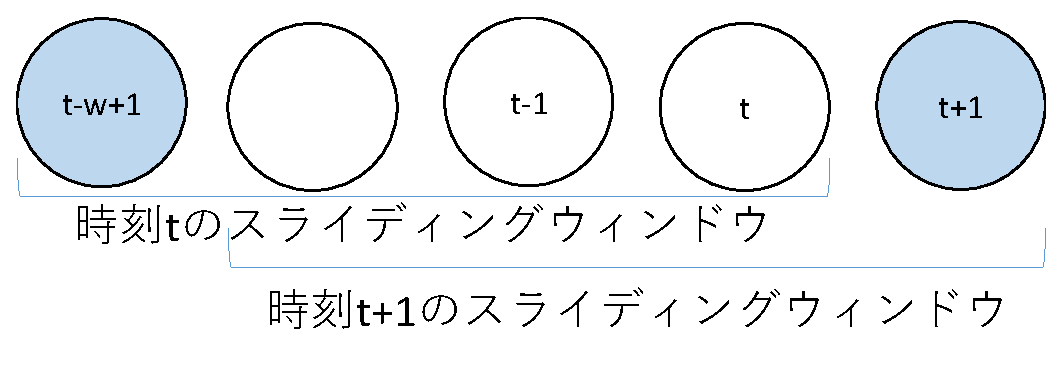
\includegraphics[clip,width=\linewidth]{img/sw.eps}
    \caption{スライディングウィンドウモデル}
    \label{sw}
  \end{center}
\end{figure}

CTS問題は,多数のユーザのテキストストリームを保持したデータベース$D$とクエリユーザ$V$のテキストストリームが与えられて,
毎時刻クエリ$V$とのユーザ間類似度$\mbox{sim}(V_T,U_T)$が閾値$\epsilon_u$以上であるすべてのユーザ$U$を$D$から検索する
継続的なレンジ探索である.したがって,スライディングウィンドウが変化する度に類似度判定結果を更新することが要求される.

ここでテキスト集合$V_T,U_T$間の類似度 $\mbox{sim}(V_T,U_T)$は以下のように定義される.
\begin{enumerate}
\item $V_T$と$U_T$の類似テキストペア間に辺を張り2部グラフ$G(V_T,U_T)$を構成する.
ここで2つのテキスト$o\in V_T,o'\in U_T$が類似テキストペアとなる条件は,$o,o'$を単語集合と見なした時に
そのJaccard類似度
\begin{align}
\label{match}
\tau (o,o')=\frac{|o\cap o'|}{|o\cup o'|}
\end{align}
が$\tau (o,o')\geq \mbox{閾値}\epsilon_{doc}$という条件を満たすことである.直感的には,
共通単語を多く保有するテキストペアが類似テキストペアとなる.閾値$\epsilon_{doc}$はレンジ探索の際に指定されるパラメータとなる.
\item グラフ$G$の最大マッチング$M$のサイズ$|M|$を$\mbox{sim}(V_T,U_T)$とする.
\end{enumerate}

なお,上記で説明した問題は単位時間毎にテキストが投稿されるとしているが,本稿で扱うすべてのアルゴリズムは数単位時間ごとにテキストが投稿されるような,ユーザごとに一定でない時間間隔でテキストが投稿される場合にも対応可能である.

\section{近似レンジ探索}\label{kinjirange}
CTS問題は毎時刻スライディングウィンドウの内容が変化するため,クエリユーザ$V$とデータベース上のすべてのユーザ$U$との類似判定結果を毎時刻更新する必要がある.よって,最大マッチングを毎時刻求める必要がある.
しかし,データベース上の全ユーザに対して存在する二部グラフの最大マッチングを毎時刻求めることは計算量が大きくなってしまい困難である.そこで久保ら\cite{kubo}の研究でああるように本研究でも類似の定義をユーザ間の最大マッチングサイズが閾値$\epsilon_u$を超えるのではなく,ユーザ間の極大マッチングサイズが閾値$\epsilon_u$を超えるかとして扱う.
類似度に極大マッチングサイズを用いれば,一度マッチングが成立したテキストペア$(o,o')$はそのどちらかがスライディングウィンドウから離脱するまでマッチングを維持でき,マッチング判定の処理を省略することができるので,類似度の算出に必要な計算量が小さくなると考えられる.


\section{ユーザ間類似度}
以上より本問題は極大マッチングサイズをもとにユーザ間類似度を決定しているが,Zhangら\cite{zhang2021clustering}は異なる基準を用いてユーザ間類似度を定義している.
Zhangらの研究では,CTS問題と同様にJaccard類似度が閾値以上になるテキストペアに辺を張り二部グラフを構築しているが,極大マッチングサイズではなく,二部グラフの最大重みマッチングサイズをユーザ間類似度としている.つまりCTS問題ではJaccard類似度が閾値$\epsilon_{doc}$となるテキストペアをすべて同じ価値としてみなしているが,Zhangらの研究ではJaccard類似度を重みととらえ,テキストペア自体に価値を設定している.最大重みマッチングを用いることでより正確にユーザ間類似度を測ることができると考える.

しかし,\ref{kinjirange}節であるように最大マッチングを求めることは計算量的に困難である.これが最大重みマッチングの場合,さらに計算量が大きくなることが予想される.よって計算量の観点から本問題のユーザ間類似度に極大マッチングサイズを用いることは妥当だと考える.

---

多重集合

を表すアルファベットϕ に対して,その要素を0 個以上含むも
のが集合となる.通常,集合は同じ種類の要素を1つしか含ま
ない.集合を同じ種類の要素を複数持てるようにしたものを多
重集合という.つまり,{a, a, b, c, d, d, d} というような集合
である.

\section{多重集合}
一般にオブジェクトの集まりを集合と呼ぶ.例えば\{a, b, c\}はアルファベットを要素とする集合である.一般的には要素群を表すアルファベット$\phi$に対して,その要素を0個以上含むものが集合となる.通常,集合は同じ種類の要素を1つしか含まない.集合を同じ種類の要素を複数持てるようにしたものを多重集合という.つまり,\{a, a, b, c, d, d, d\}というような集合である.


\section{Jaccard係数}
集合間で類似検索を行うには集合がどれだけ似ているのかを表す集合間類似度が定義されている必要がある.そのうちの1つとして,Jaccard係数がある.
Jaccard係数は,ある集合$A$と別の集合$B$について,以下の式\ref{eq:sim}で定義される.
\begin{equation}
\label{eq:sim}
\mathrm{sim}(A,B)=  \frac {|A \cap {B} |} {|A \cup {B}| }
\end{equation}

つまり,Jaccard係数は2つの集合に含まれている要素のうち共通要素が占める割合を表している.
例えば,$A=\{a,c,d,f,g\}$,$B=\{a,b,c,e,g,h,i\}$というような2つの集合が存在するとすると,${A \cup {B} }=\{a,b,c,d,e,f,g,h,i\}$,$ {A \cap {B} }=\{a,c,g\}$となり,類似度$sim(A,B)=0.375$となる.

そして,Jaccard係数を多重集合に拡張したものを拡張Jaccard係数と言う(式 \ref{eq:exjaccard}).
\begin{equation}
\label{eq:exjaccard}
\mathrm{sim}(A,B)=  \frac {\sum{\mathrm{min}\{a_i,b_i\}}} {\sum{\mathrm{max}\{a_i,b_i\}} }\\
\end{equation}

ここで,$a_i$は集合$A$が要素$i∈\phi$を含む個数である.

\section{Min-hash}
Min-hashとは,集合に対する確率的なハッシュ関数であり,Jaccard係数を用いた集合間類似検索を高速化するための技術である \cite{Minhash}.クエリとデータベースかの集合間でJaccard係数を計算することはJaccard係数計算のオーバーヘッドが大きい.その問題を改善し,Jaccard係数を高速に近似計算する方法として,Min-hashという計算方法が考えられた.Min-hashは計算されたハッシュ値が一致する確率はJaccard係数と一致するという性質を持ち,類似集合ほどハッシュ値が一致しやすいという良い性質を持つ(式\ref{eq:jaccard}).

(1)のハッシュ値計算手法を例を用いて説明する.まず,図\ref{fig:2wariate}のように,アルファベット\{a,b,c,d\}に多重度が2である時の数値をランダムに割り当てる.
\begin{figure}[H]
  \centering
  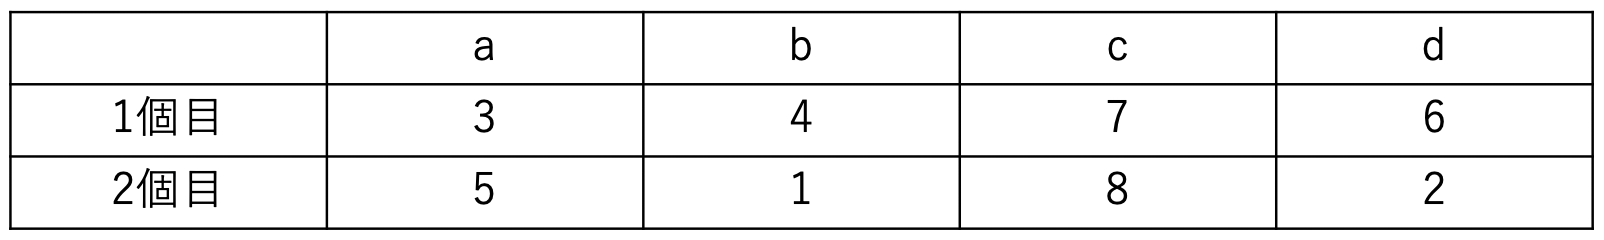
\includegraphics[width=15cm]{multi22.png}
  \caption{多重集合のハッシュ値表}
  \label{fig:2wariate}
\end{figure}

多重集合$A =\{a,b,b,c,c,d,d\}$とする.多重集合$A$に対して,図\ref{fig:2wariate}の割り当て表を用いて数値を割り当てる.そして,その中の最小値がMin-Hashによるハッシュ値となる(図\ref{fig:255}).

\begin{figure}[H]
  \centering
  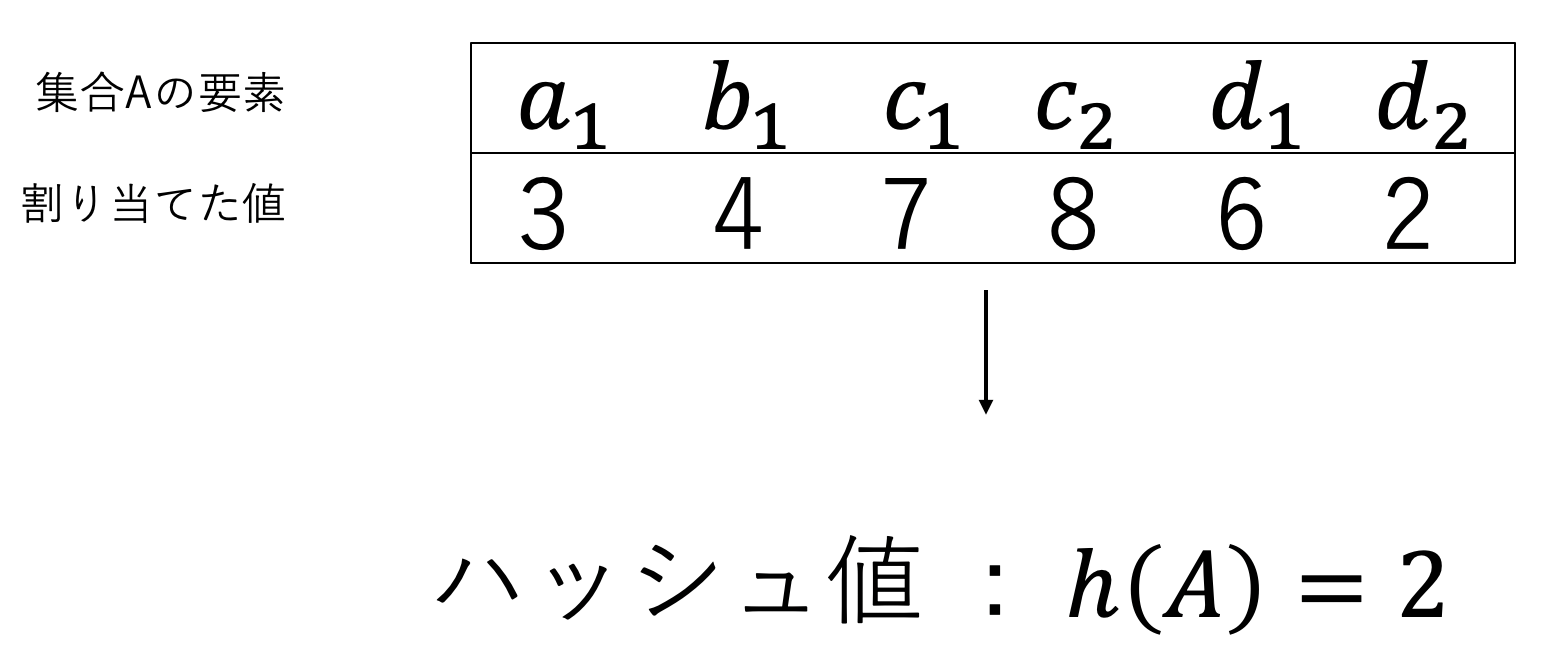
\includegraphics[width=15cm]{255.png}
  \caption{多重集合のハッシュ値計算}
  \label{fig:255}
\end{figure}

\section{スライディングウインドウモデル}
時刻$t$における集合を$A_t=\{e_{t-w+1},e_{t-w+2},\cdots,e_t\}$とする.$w$はスライディングウインドウの幅であり,
$A_t$は$w$個の要素で構成される.また,$A_t$の要素は到着時間順に並んでいる.図\ref{fig:window}では,$w=4$の時
に3つの時刻$t$,$t+1$,$t+2$に対する集合$A_t,A_{t+1},A_{t+2}$を図示している.そして,時刻によってスライディングウインドウは変化していく.
例えば,図\ref{fig:window}のようにデータストリーム$\{a,f,h,e,k,q,o,g\}$となっていて,ウインドウサイズ$w=4$とすると,時刻$t$では,
$A_{t}=\{e_{t-3},e_{t-2},e_{t-1},e_t\}$であり,時刻$t +1$では,$A_{t+1}=\{e_{t-2},e_{t-1},e_t,e_{t+1}\}$となる.

3. 問題点

3.1. Minlistの探索回数の増大

そもそもなぜMinlistの探索が必要なのか?

Minlistは,探索回数が多い.多重度のヒストグラムは要素Nが到着したときの到着時刻tをすべて記録している.しかしこの実装だとヒストグラムの要素数はスライディングウィンドウのサイズになる.このヒストグラムの到着時刻は.割り当て値であるハッシュ値の更新に使用する.要素γがウィンドウ内に存在する間、γ,et+1 間にラベルがl(et+1)となる要素がn個ある。よって、要素γ の存在尾期間中のet+1の割り当て値はπ(l(et+1)n) より大きくならなない。よってであれば,要素γ をMinlist から削除してよい.最後にMinlist の一番後ろにet+1 を挿入し,π(et+1) がMinlistの最小値を更新するかをチェックする.現在のハッシュ値よりπ(et+1) が小さいならば,ハッシュ値を更新する.

3.2. 割り当て表のメモリ割り当てのメモリが大きい

Min-hashを割り当てるためのハッシュ値の割り当て表のサイズは要素の種類数×多重度になる.しかし割り当て値の修正を行っているため,多重度が大きくなればなるほど割り当て値の変動する確率が下がる.そのため割り当て表はサイズが大きくなればなるほど意味を持たない割り当て値を多く持つことになりメモリ使用量に無駄が生じる.

3.3. ヒストグラムのメモリ割り当てのメモリが大きい

ヒストグラムのサイズは,要素の種類数の数だけ配列のサイズを確保する必要がある.ストリームデータが複数個になると,その数だけヒストグラムのメモリを確保する必要がある.また,スライディングウィンドウのサイズに対して要素の種類数が多いとヒストグラムの要素が0である比率が大きくなる.実質的に意味を持たない要素が多くなる.

4. 提案手法

3.1. Minlistの探索にSerch Limitを設ける



3.2. Active Indexを用いた割り当て表の作成

3.3. Count-Min Sketchを用いた多重度の近似ヒストグラムの作成

\chapter{従来手法}
% !TEX root = Sotsuron_main_v3.tex
%%Chap3
テキストを集合の要素とした類似検索にはEfstathiadesらが扱ったSTPSJoin問題\cite{efstathiades}がある.STPSJoin問題は静的なテキスト集合から類似するユーザペアの集合を検索するJoin問題である.一方でCTS問題は動的なテキスト集合を扱い,クエリとなるユーザと類似度が閾値以上であるユーザを検索する点が異なる.また,STPSJoin問題の類似度は相手のユーザが持つテキストの中に類似するテキストが一つでもあるテキストの数の割合である.一方でCTS問題の類似度は類似するテキストのペア同士で辺を結ぶことで構築される二部グラフの極大マッチングのサイズである.このように類似度の求め方も異なる.
本章では,久保らが提案したCTS問題に対する類似検索アルゴリズムである遅延評価法を説明する.遅延評価法の疑似コードをAlgorithm \ref{alg:statedelay}に示す.この遅延評価法はマッチング判定を行う際,ユーザ間類似度を正確に求めるのではなく,ユーザ間類似度が$\epsilon_u$を越えるかのみを調べることによってマッチング判定回数の削減を行い,高速化を狙ったアルゴリズムである.
遅延評価法では以下のようにクエリユーザ$V$のスライディングウィンドウ$V_{T}$内のそれぞれのテキストを以下の3つの集合に分類する.
\begin{itemize}
  \item $V_{M}$ マッチングすることが確定したテキスト集合
  \item $V_{NM}$ マッチングしないことが確定したテキスト集合
  \item $V_{UM}$ マッチングするか未定なテキスト集合
\end{itemize}
さらに,ユーザごとにスライディングウィンドウ$U_{T}$内のそれぞれのテキストを以下の2つの集合に分類する.
\begin{itemize}
  \item $U_{M}$ マッチングすることが確定したテキスト集合
  \item $U_{UM}$ マッチングするか未定なテキスト集合
\end{itemize}

%そのために,以下の二つを行う.
以上の定義より$|V_M|=|U_M|$が成り立つ.
\begin{itemize}
    \item 「マッチングすることが確定した」とはただ1つのテキストとペアになっている状態を指す.
    \item 「マッチングしないことが確定した」とはペアになるための条件を満たすテキストが1つも存在しない状態を指す.つまりマッチングペアの対象のすべてのテキストとのJaccard類似度は計算済みである.
    \item 「マッチングするか未定」とはマッチングペアの対象のすべてのテキストとのJaccard類似度の算出が済んでいない状態であり,マッチングする可能性が残っているテキストという意味である.
\end{itemize}

この遅延評価法は,
\begin{itemize}
    \item 類似となる条件 $|V_M|\geq\epsilon_u$
    \item 非類似となる条件 $|V_{NM}|>W-\epsilon_u$
\end{itemize}
のどちらかの条件を満たすまでマッチング判定をすることによって必要以上のマッチング判定処理を省き,ユーザ間類似度が閾値$\epsilon_u$以上になるユーザを効率よく見つけ出すことを狙っている.
遅延評価法の処理の流れを図\ref{fig:lazy}に示す.
$V$,$U$のスライディングウィンドウに入ってくるテキストを$\mbox{IN}_V$,$\mbox{IN}_U$,スライディングウィンドウから離脱するテキストを$\mbox{OUT}_V$,$\mbox{OUT}_U$とする.
\begin{figure}[htb]
    \centering
    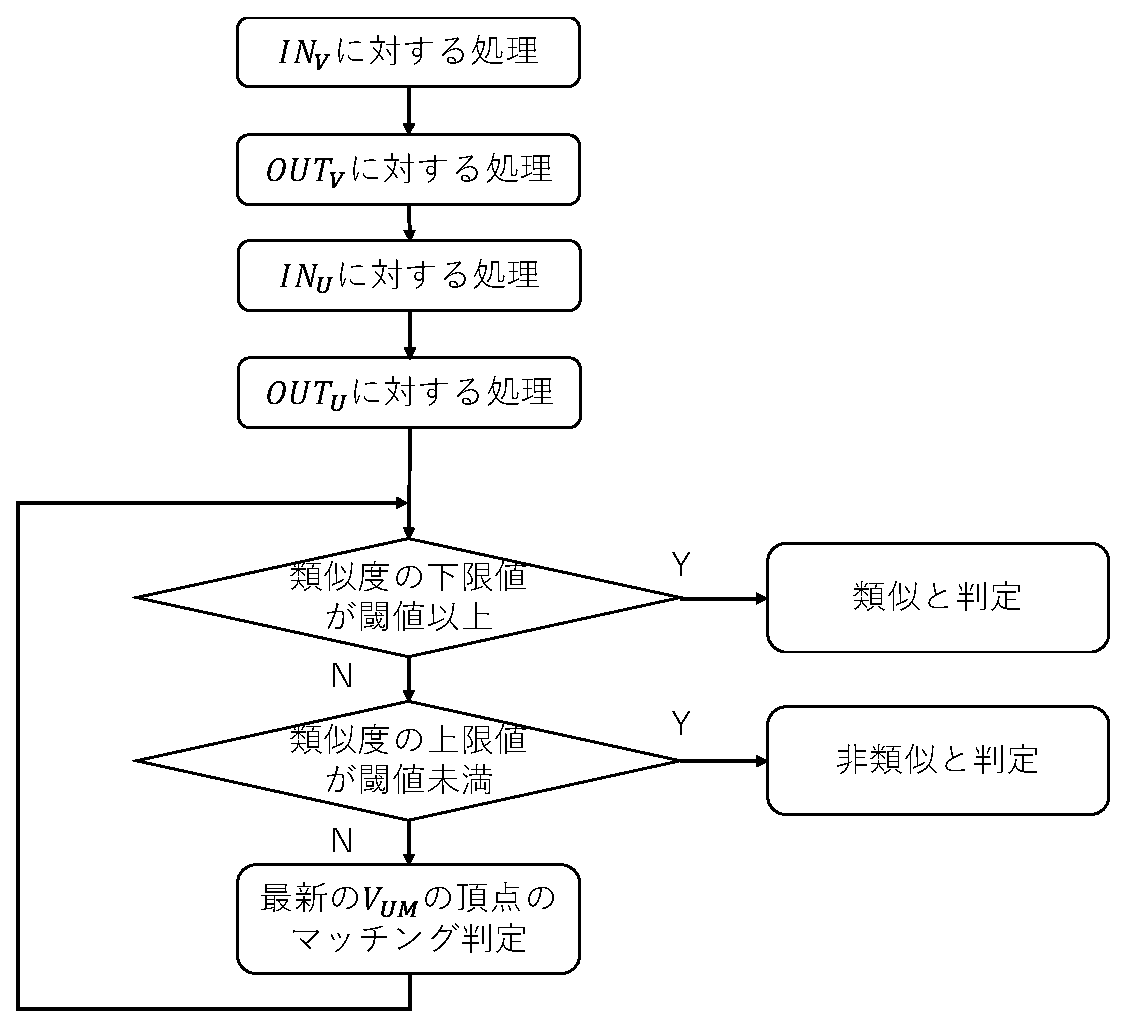
\includegraphics[width=8.7cm]{img/delay.eps}
    \caption{遅延評価法の処理の流れ}
    \label{fig:lazy}
\end{figure}

\section{\texorpdfstring{$\mbox{IN}_{V}$} に対する処理}
クエリ$V$のテキストストリームに新しいテキスト$\mbox{IN}_V$が到着し,$\mbox{IN}_V \in V_{UM}$とする.

\section{\texorpdfstring{$\mbox{OUT}_V$} に対する処理}
最も古いテキスト$\mbox{OUT}_V$を$V_M$,$V_{NM}$,$V_{UM}$の所属している集合から除外する.特に$\mbox{OUT}_V \in V_{M}$であった時は,$\mbox{OUT}_V$のマッチング相手であったユーザ$U$のテキスト$O_U$はマッチング相手がいなくなることから$O_U$を$U_{M}$から除外する.さらに,$O_U$は$V_{NM}$のテキストとマッチングする可能性があるため,$O_U$と$V_{NM}$のテキストとのマッチング判定を行う.
\begin{itemize}
    \item $V_{NM}$内のテキスト$O_V$とマッチングした場合 : $O_V \in V_{M},O_U \in U_{M}$
    \item マッチングしなかった場合 : $O_U \in U_{UM}$
\end{itemize}
とする.

\section{\texorpdfstring{$\mbox{IN}_U$} に対する処理}
ユーザ$U$のテキストストリームに新しいテキスト$\mbox{IN}_U$が到着する時,$\mbox{IN}_U$と$V_{NM}$のいずれかのテキスト同士がマッチングする可能性が発生することから,
$\mbox{IN}_U$を起点とした$V_{NM}$内の各テキストに対するマッチング判定を行う.
\begin{itemize}
    \item $V_{NM}$内のテキスト$O_V$とマッチングした場合 : $O_V \in V_{M},\mbox{IN}_U \in U_{M}$
    \item マッチングしなかった場合 : $\mbox{IN}_U \in U_{UM}$
\end{itemize}
とする.

\section{\texorpdfstring{$\mbox{OUT}_U$} に対する処理}
スライディングウィンドウ内の最も古いテキスト$\mbox{OUT}_U$を$U_M,U_{UM}$の所属している集合から除外する.特に$\mbox{OUT}_U \in U_M$であった時,$\mbox{OUT}_U$とマッチングしていたテキスト$O_V$を$O_V \in V_{UM}$とする.

\section{類似・非類似の判定処理}
ここでは各時刻Tでユーザ間類似度が$\epsilon_u$を超えるかを判定するプロセスを示している.
$V_{M}$($=U_{M}$)の大きさは常に$\mbox{sim}(V_{T},U_{T})$以下であることから,$V_{M}$の大きさがユーザ間類似度の下限値といえる.さらに$V_{NM}$に所属するテキストはマッチングすることはないため,スライディングウィンドウの大きさ$W$を用いて$W-|V_{NM}|$がユーザ間類似度の上限値となる.したがって,ユーザ間類似度を正確に求めるのではなく,類似となる条件式
\begin{equation}
\label{ruiji}
|V_{M}| \geq \epsilon_u
\end{equation}
または,非類似となる条件式
\begin{equation}
\label{hiruiji}
W - |V_{NM}| < \epsilon_u
\end{equation}
のどちらかを満たすまでマッチング判定を行えばよい.
%そこで,$|V_M| \geq \epsilon_u$,または$w-|V_{NM}| \leq \epsilon_u$のいずれかが成立するまで
そこで,式(\ref{ruiji})または式(\ref{hiruiji})のいずれかが成立するまで
%$V_{UM}$に所属するテキストを1つ取り出し,$U_{UM}$に所属するテキストとのマッチング判定を繰り返し行う.
$V_{UM}$の各テキストを起点とした$U_{UM}$内のテキストに対する以下のマッチング判定処理を繰り返し行う.

\begin{itemize}
    \item $V_{UM}$のテキスト$O_V$と$U_{UM}$のテキスト$O_U$がマッチングした場合,$O_V \in V_M,O_U \in U_M$とする.この時,$V_M$の大きさが1増加する.
    \item $V_{UM}$のテキスト$O_V$が$U_{UM}$のどのテキストともマッチングしなかった場合,$O_V \in V_{NM}$とする.このとき$V_{NM}$の大きさが1増加する.
\end{itemize}

%極大マッチングサイズの上限と下限の情報を利用して,処理の枝刈りを行い,高速化を図っている.
%データベースのテキストストリームごとに以下を設定する.



\section{マッチング判定を行うペアの順番}
\label{order_matching}
ユーザ間類似度を求める際に行うマッチング判定は,$V_{UM}$内のテキストと$U_{UM}$内のテキスト同士でマッチング判定を行うが,それぞれの集合内のどのテキストからマッチング判定を行うかは自由度が存在する.そこで遅延評価法では常に新しいテキストから優先してマッチング判定を行う.このとき,新しいテキスト同士がマッチングすることで長時間マッチングの関係が維持でき,どちらか片方のテキストがスライディングウィドウを離脱したときのマッチング判定のやり直しの回数の削減が見込める.
  %\item 古いテキストほどマッチング判定対象になりにくく,マッチング判定をされないままスライディングウィンドウを離脱するテキストが増えると考えられ,マッチング判定回数の削減が見込める.
%\end{itemize}
%ということがあげられる.

\begin{comment}
\begin{figure}[!t]
\begin{algorithm}[H]
    \caption{遅延評価法}
    \label{alg1}
    \begin{algorithmic}[1]
    \STATE $\mbox{IN}_V\in V_{UM}$とする
    \STATE $\mbox{OUT}_V$をスライディングウィンドウから離脱させる
    \IF {$\mbox{OUT}_V\in V_{M}$}
        \STATE $O_U\leftarrow Pair(\mbox{OUT}_V)$
        \FOR {$O_V\in V_{NM}$}
            \IF {($\tau(O_V,O_U)\geq \epsilon_{doc}$)}
                \STATE $O_V$と$O_U$がマッチング
                \STATE break
            \ENDIF
        \ENDFOR
    \ENDIF
    \FOR {$O_V\in V_{NM} $}
        \IF {($\tau(O_V,\mbox{IN}_U)\geq \epsilon_{doc}$)}
            \STATE $O_V$と$\mbox{IN}_U$がマッチング
            \STATE break
        \ENDIF
    \ENDFOR
    \STATE $\mbox{OUT}_U$をスライディングウィンドウから離脱させる
    \IF{$\mbox{OUT}_U\in U_{M}$}
        \STATE $Pair(\mbox{OUT}_U)\in V_{UM}$とする
    \ENDIF
    \WHILE {$|V_M| < \epsilon_u$ AND $|V_{NM}| \leq (w-\epsilon)$}
        \STATE $O_V \leftarrow V_{UM} $の一番新しいテキスト
        \FOR{$O_U \in U_{UM}$}
            \IF {($\tau(O_V,O_U)\geq \epsilon_{doc}$)}
               \STATE $O_V$と$O_U$がマッチング
            \STATE break
            \ENDIF
        \ENDFOR
        \IF{$O_V$がどの$U_{UM}$ともマッチングしない}
            \STATE $O_V\in V_{NM}$とする
        \ENDIF
    \ENDWHILE
    \IF {($|V_M|  < \epsilon_u$)}
        \STATE Not Similar
    \ENDIF
    \IF {($|V_M|  \geq \epsilon_u$)}
        \STATE Similar
    \ENDIF
\end{algorithmic}
\end{algorithm}
\end{figure}
\end{comment}



\begin{algorithm}[H]
 \caption{遅延評価法}
 \label{alg:statedelay}
 \begin{algorithmic}[1]
  \State $\mbox{IN}_V\in V_{UM}$とする
  \State $\mbox{OUT}_V$をスライディングウィンドウから離脱させる
  \If {$\mbox{OUT}_V\in V_{M}$}
    \State $O_U\leftarrow Pair(\mbox{OUT}_V)$
    \For {$O_V\in V_{NM}$}
    \If {($jac(O_V,O_U)\geq \epsilon_{doc}$)}
      \State $O_V$と$O_U$がマッチング
      \State break
    \EndIf
    \EndFor
  \EndIf
  \For {$O_V\in V_{NM} $}
  \If {($jac(O_V,\mbox{IN}_U)\geq \epsilon_{doc}$)}
  \State $O_V$と$\mbox{IN}_U$がマッチング
  \State break
  \EndIf
  \EndFor
  \State $\mbox{OUT}_U$をスライディングウィンドウから離脱させる
  \If{$\mbox{OUT}_U\in U_{M}$}
    \State $Pair(\mbox{OUT}_U)\in V_{UM}$とする
  \EndIf
  \While {$|V_M| < \epsilon$ AND $|V_{NM}| \leq (w-\epsilon)$}
    \State $O_V \leftarrow V_{UM} $の一番新しいテキスト
    \For{$O_U \in U_{UM}$}
      \If {($jac(O_V,O_U)\geq \epsilon_{doc}$)}
        \State $O_V$と$O_U$がマッチング
        \State break
      \EndIf
    \EndFor
    \If{$O_V$がどの$U_{UM}$ともマッチングしない}
      \State $O_V\in V_{NM}$とする
    \EndIf
  \EndWhile
  \If {($|V_M|  < \epsilon$)}
  \State Not Similar
  \EndIf
  \If {($|V_M|  \geq \epsilon$)}
  \State Similar
  \EndIf
 \end{algorithmic}
 \end{algorithm}

\chapter{転置インデクス}
\label{chap:ii}
%%Chap4.tex
%ここでは静的なテキスト集合を対象とした転置インデクスを想定する


本章では本問題に対する転置インデクスの管理・利用について説明する.

遅延評価法はマッチング判定の際に,共通単語を1つも持たないテキストに対してもマッチング判定を行っている.共通単語を1つも持たないとき,Jaccard類似度は0となり類似判定をする必要がない.転置インデクスを用いると共通単語を含むテキストのみを参照することができ,Jaccard類似度が0になるテキストへのマッチング判定を避けることができる.よって遅延評価法に転置インデクスを用いたマッチング判定処理を導入することで類似性判定の処理の高速化を狙う.

\section{データ構造}
マッチング判定はスライディングウィンドウ内のテキストを対象としているので,ユーザ$U$が持つ時刻$T$でのテキスト集合$U_T$は,スライディングウィンドウの大きさ$W$を用いて$U_T=\{u_{T-W+1}, u_{T-W+2}, \cdots u_T\}$と表せる.そしてテキスト$u_T$が持つ単語は,$u_T=\{t_1, t_2, \cdots, t_{|u_T|}\}$と表せる.各テキストはそれぞれが持つ単語によって索引付けされ,単語$t_i$に対するリスト$L_i$は$\langle\mbox{ID}(u_T), f_i\rangle$と表されるテキスト情報を持ち,$\mbox{ID}(u_T)$はテキスト$u_T$が持つテキストID,$f_i$はテキスト$u_T$内の単語$t_i$の出現回数である.$u_T$のハッシュ値を計算し,その値にリスト$L_i$を対応させたハッシュテーブルを転置インデクスとする.

%あるテキスト$Q$に存在する単語を含むテキストをテキスト集合から検索す%る環境を想定し,その環境下での転置インデクスの利用方法を述べる.静%的なテキスト集合に対して転置インデクスを活用することで大規模なデー%タに対する高速な検索が実現できる.
%ここでもテキストは単語集合であるとする.

\section{構築}

静的なテキスト集合を対象とした転置インデクスであれば,テキスト集合の内容は変化せず,転置インデクスを更新する必要はない.しかし,本問題は動的なテキスト集合を扱うため転置インデクスを更新する必要がある.そのため動的なテキスト集合に適した転置インデクスのデータ構造を提案する.
テキストストリームには毎時刻スライディングウィンドウに新しいテキストが到着し,古いテキストが離脱する.このことから単語$t_i$に対応付けられるリスト$L_i$にはキューを用いる.新しいテキストが到着したときには$L_i$の先頭に追加,古いテキストが離脱するときには$L_i$の末尾からテキストを削除とすることで管理コストを抑えつつ動的なテキスト集合に対応した転置インデクスを管理できると考える.

よって転置インデクスの単語$t_i$に対するリスト$L_i$には先頭に近いほど新しいテキストが格納されることになる.転置インデクスの構成を図\ref{fig:ii}に示す.
\begin{figure}[H]
    \centering
    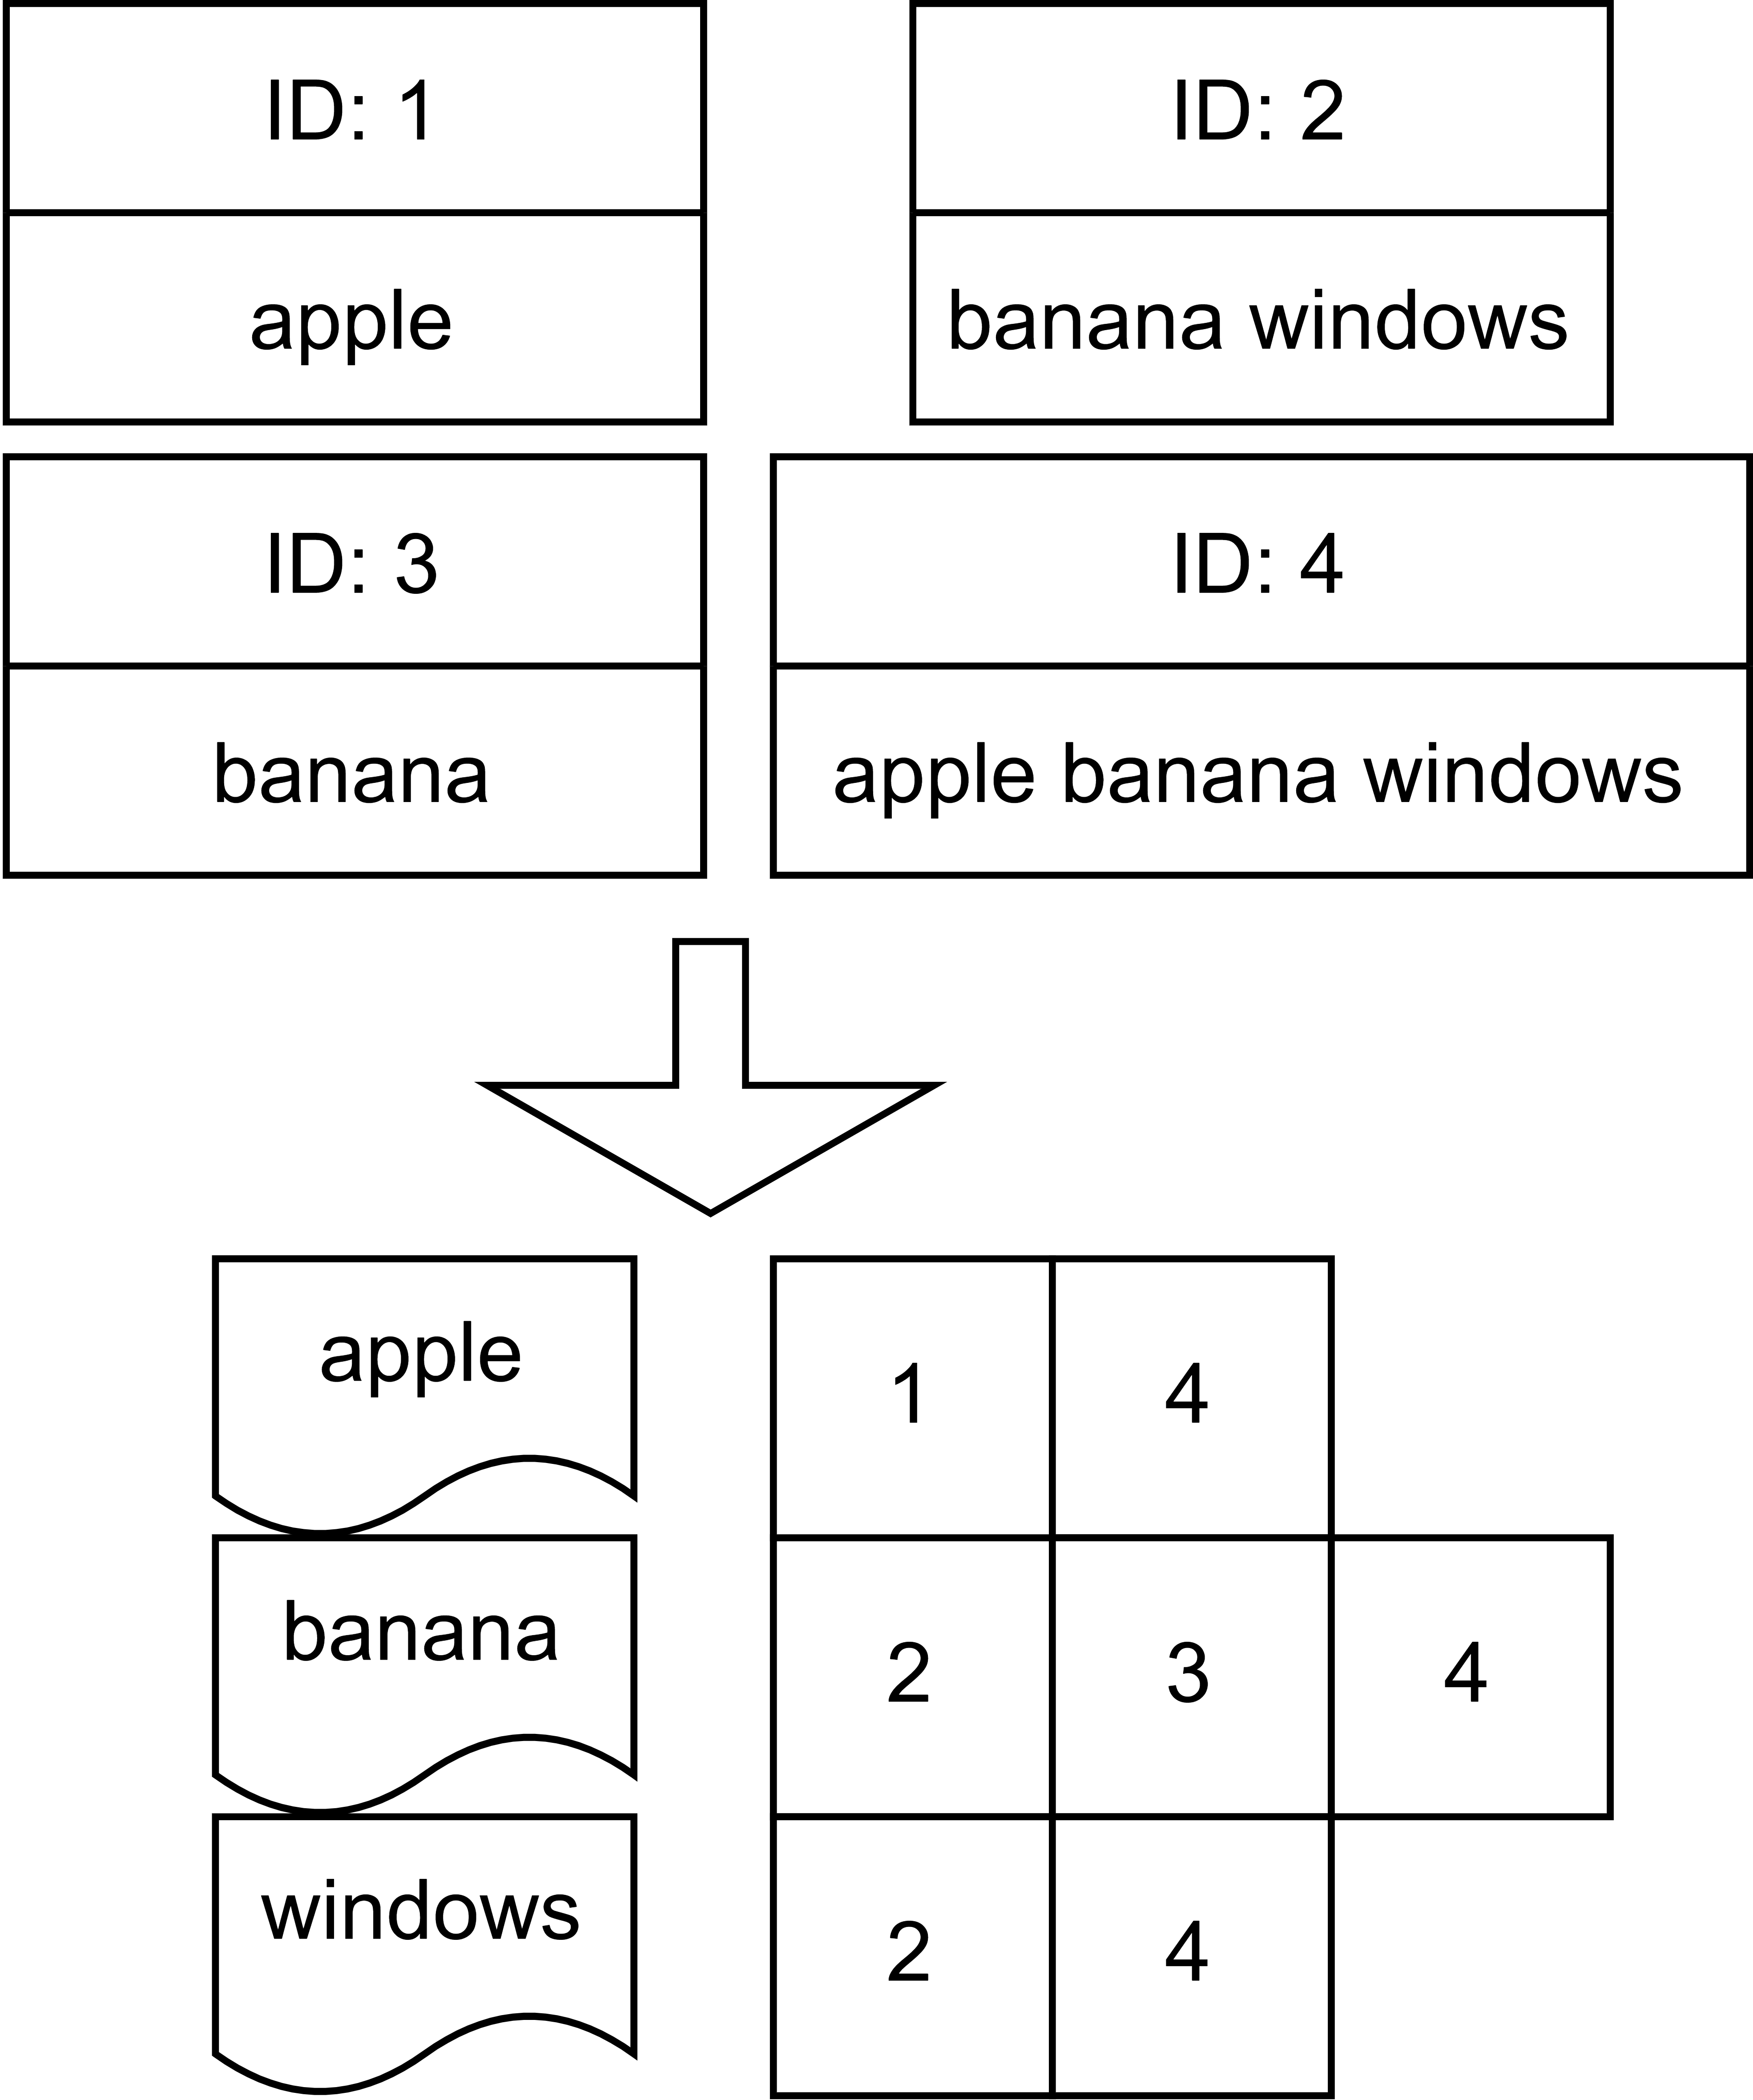
\includegraphics[width=8.7cm]{img/ii.png}
    \caption{転置インデクスの構成}
    \label{fig:ii}
\end{figure}

\section{利用}

テキスト集合$U_T$とテキスト集合$V_T$のテキストについて極大マッチングを求めることを考える.テキスト集合$V_T$に対して転置インデクス$ii_{V_T}$が構築されているとする.
まず,テキスト集合$U_T$からテキスト$u_T$を取り出す.テキスト$u_T$が持つ単語$t_1, t_2, \cdots, t_{|u_T|}$に対応するリストを$ii_{V_T}$から取得するが,ここで取得したリストを用いてテキストを参照する方法が2つ存在する.
\begin{itemize}
    \item TAAT (Term-At-A-Time)
    \begin{description}
        \setlength{\leftskip}{0.25cm}
        \item 単語単位で処理を行う.
        \begin{enumerate}[手順 1]
        \setlength{\leftskip}{0.7cm}
            \item アキュムレータ($acc$)を用意する.
            \item \label{taat:rep} $u_T$から単語$t_1$を取り出し,対応するリストに含まれる全てのテキスト情報を$acc$に追加する
            \item 手順\ref{taat:rep}をすべての単語に対して行う.
            \item $acc$が$u_T$に含まれるテキストを1つでも含むテキストの情報である.
        \end{enumerate}
        アキュムレータに追加されていくテキスト情報は$u_T$から取り出す単語の順番に依存しており,追加される順番に一貫性はない.TAATの手順を図\ref{fig:TAAT}に示す.
    \end{description}
    
    \begin{figure}[H]
        \centering
        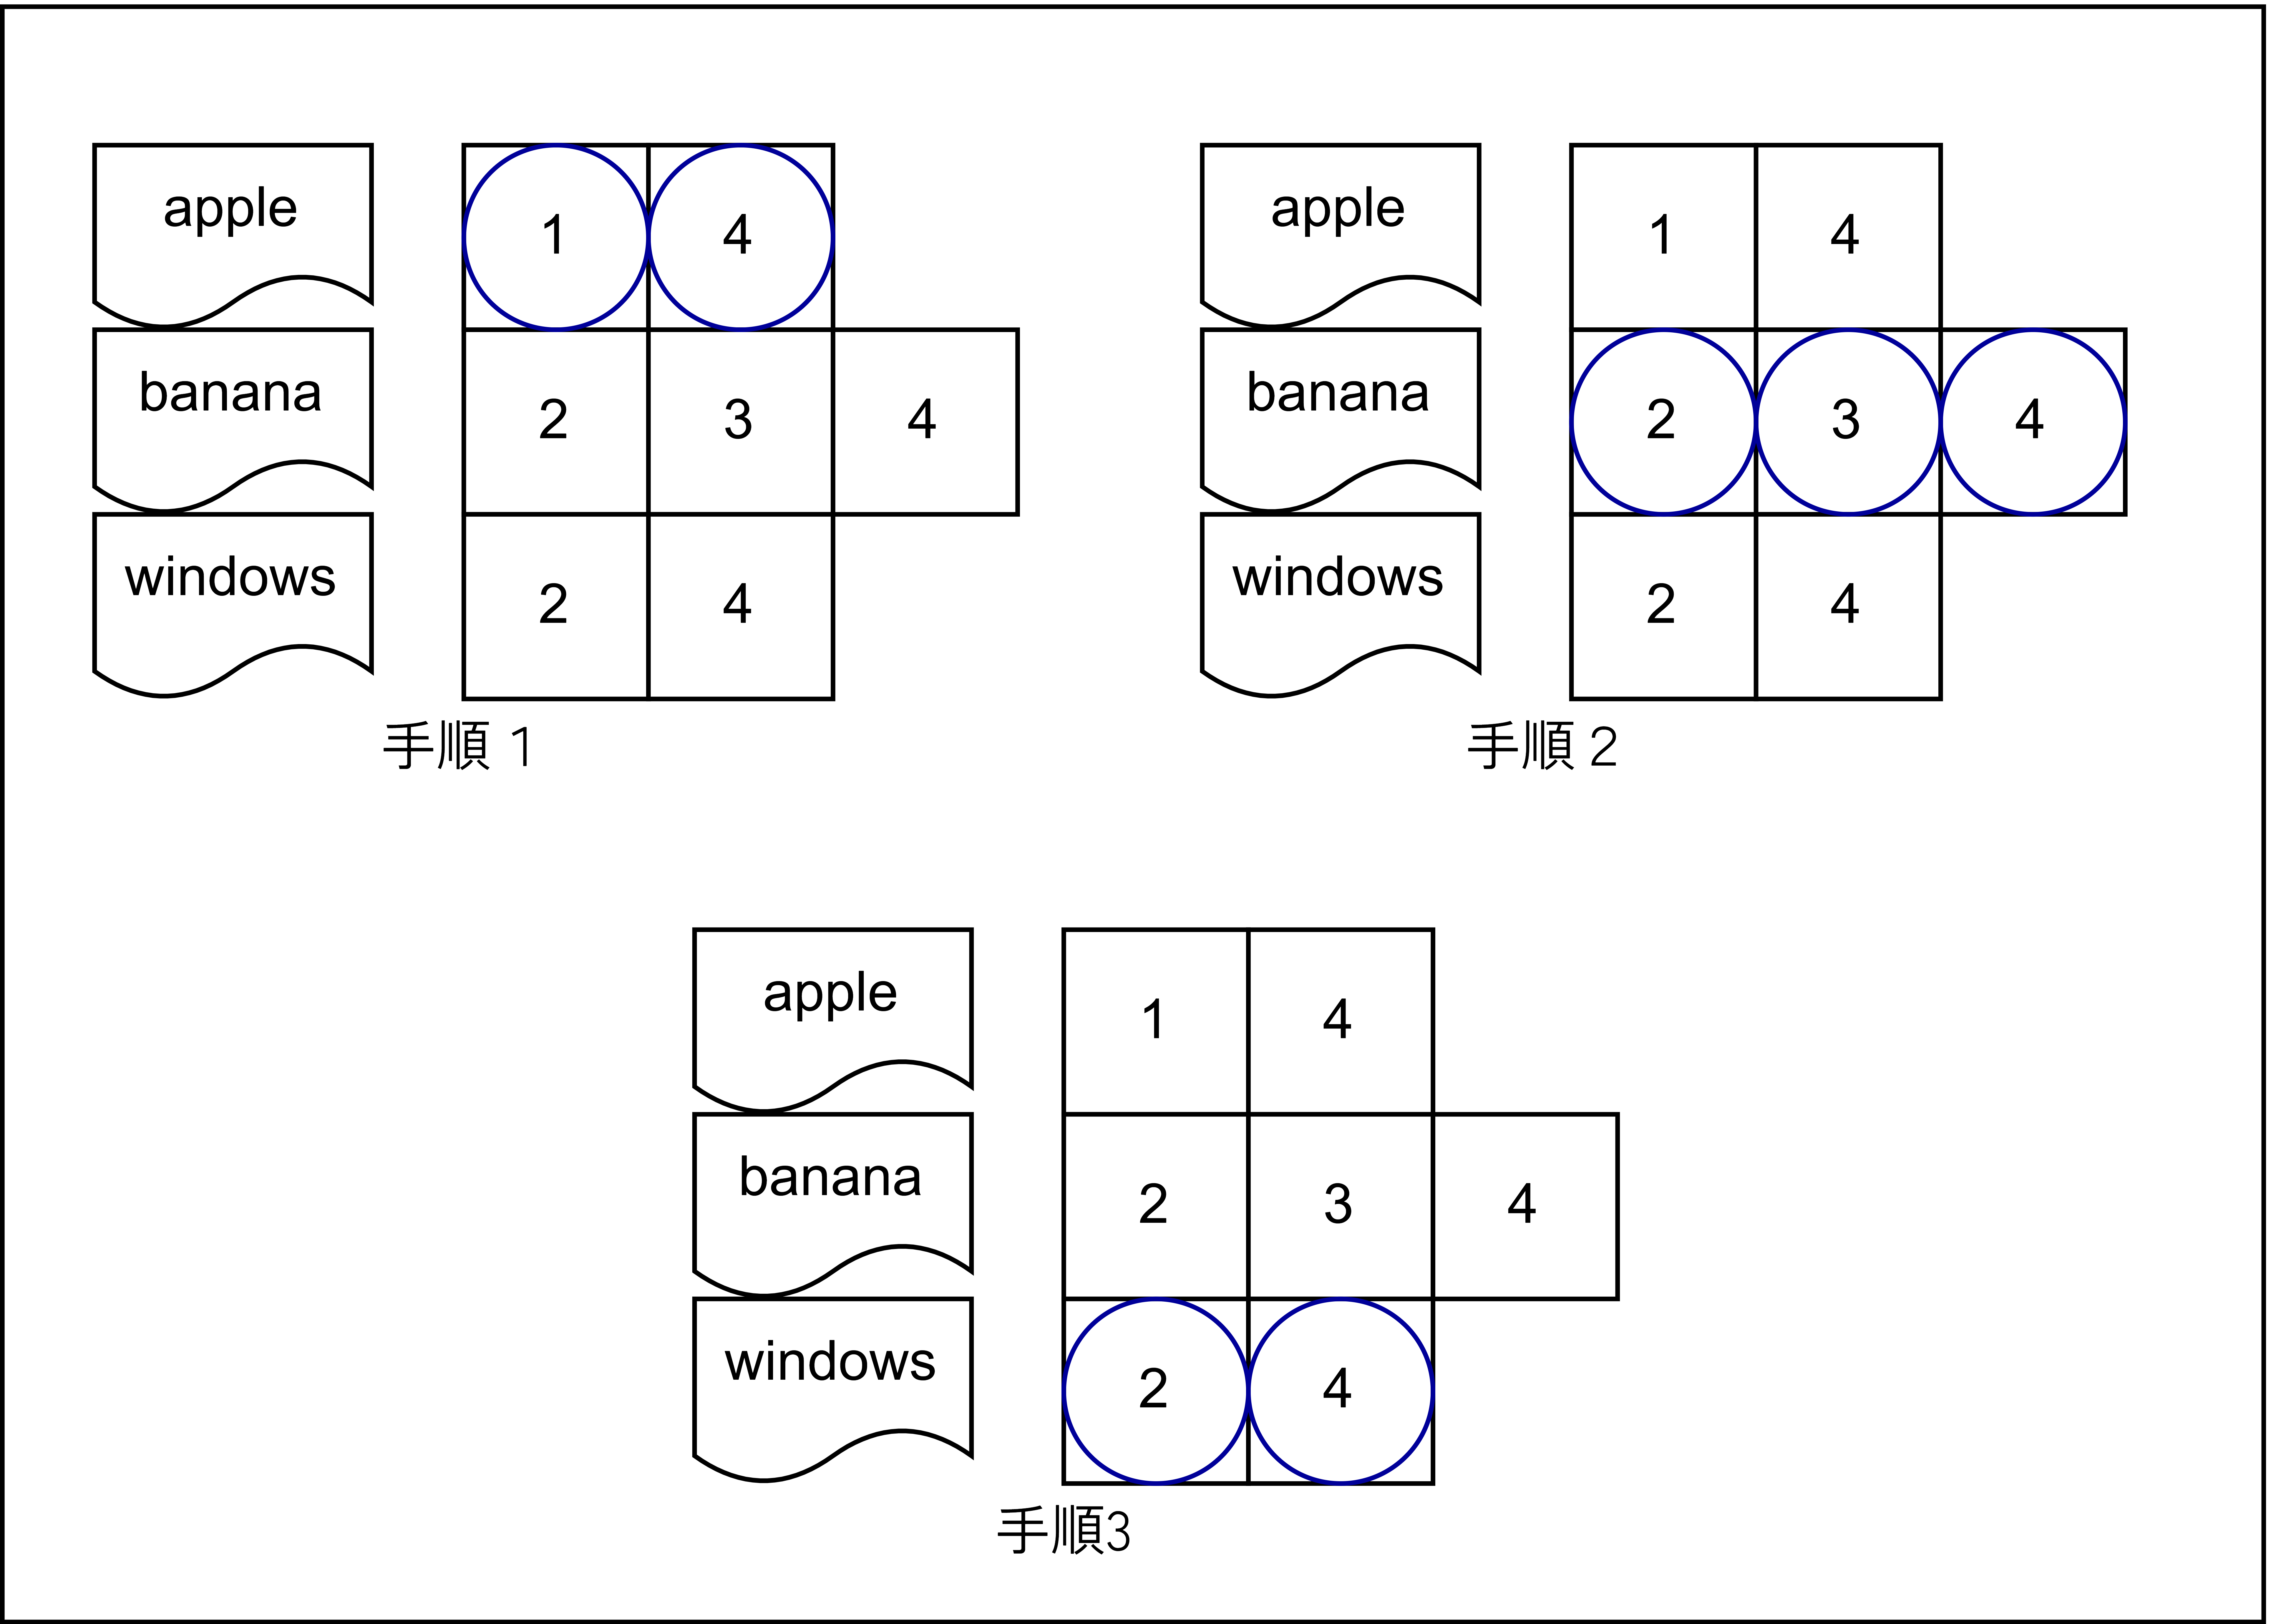
\includegraphics[width=8.7cm]{img/taat.png}
        \caption{TAATの手順}
        \label{fig:TAAT}
    \end{figure}
    
    \item DAAT (Document-At-A-Time)
    \begin{description}
        \setlength{\leftskip}{0.25cm}
        \item {テキスト単位で処理を行う.
        \begin{enumerate}[手順 1]
        \setlength{\leftskip}{0.7cm}
            %\item テキストの投稿時間が最新のテキストが根に来るようなヒープ$H$を用意する.
            \item 最も投稿時間の新しいテキストが根に来るヒープ$H$を用意する.
            \item \label{daat:rep} $u_T$から単語$t_1$を取り出し,対応するリストの先頭を$H$に追加する
            \item 手順\ref{daat:rep}をすべての単語に対して行う.
            \item \label{daat:heap}ヒープ$H$から最も新しいテキストを取り出し,所属するリストの次のテキストを再びヒープ$H$に追加する.
        \end{enumerate}
            TAATとは異なり手順\ref{daat:heap}で新しいテキストから優先してテキストを参照することが出来るため,新しいテキストからマッチング判定をすることが可能である.DAATの手順を図\ref{fig:DAAT}に示す.
        }
        
        \begin{figure}[H]
            \centering
            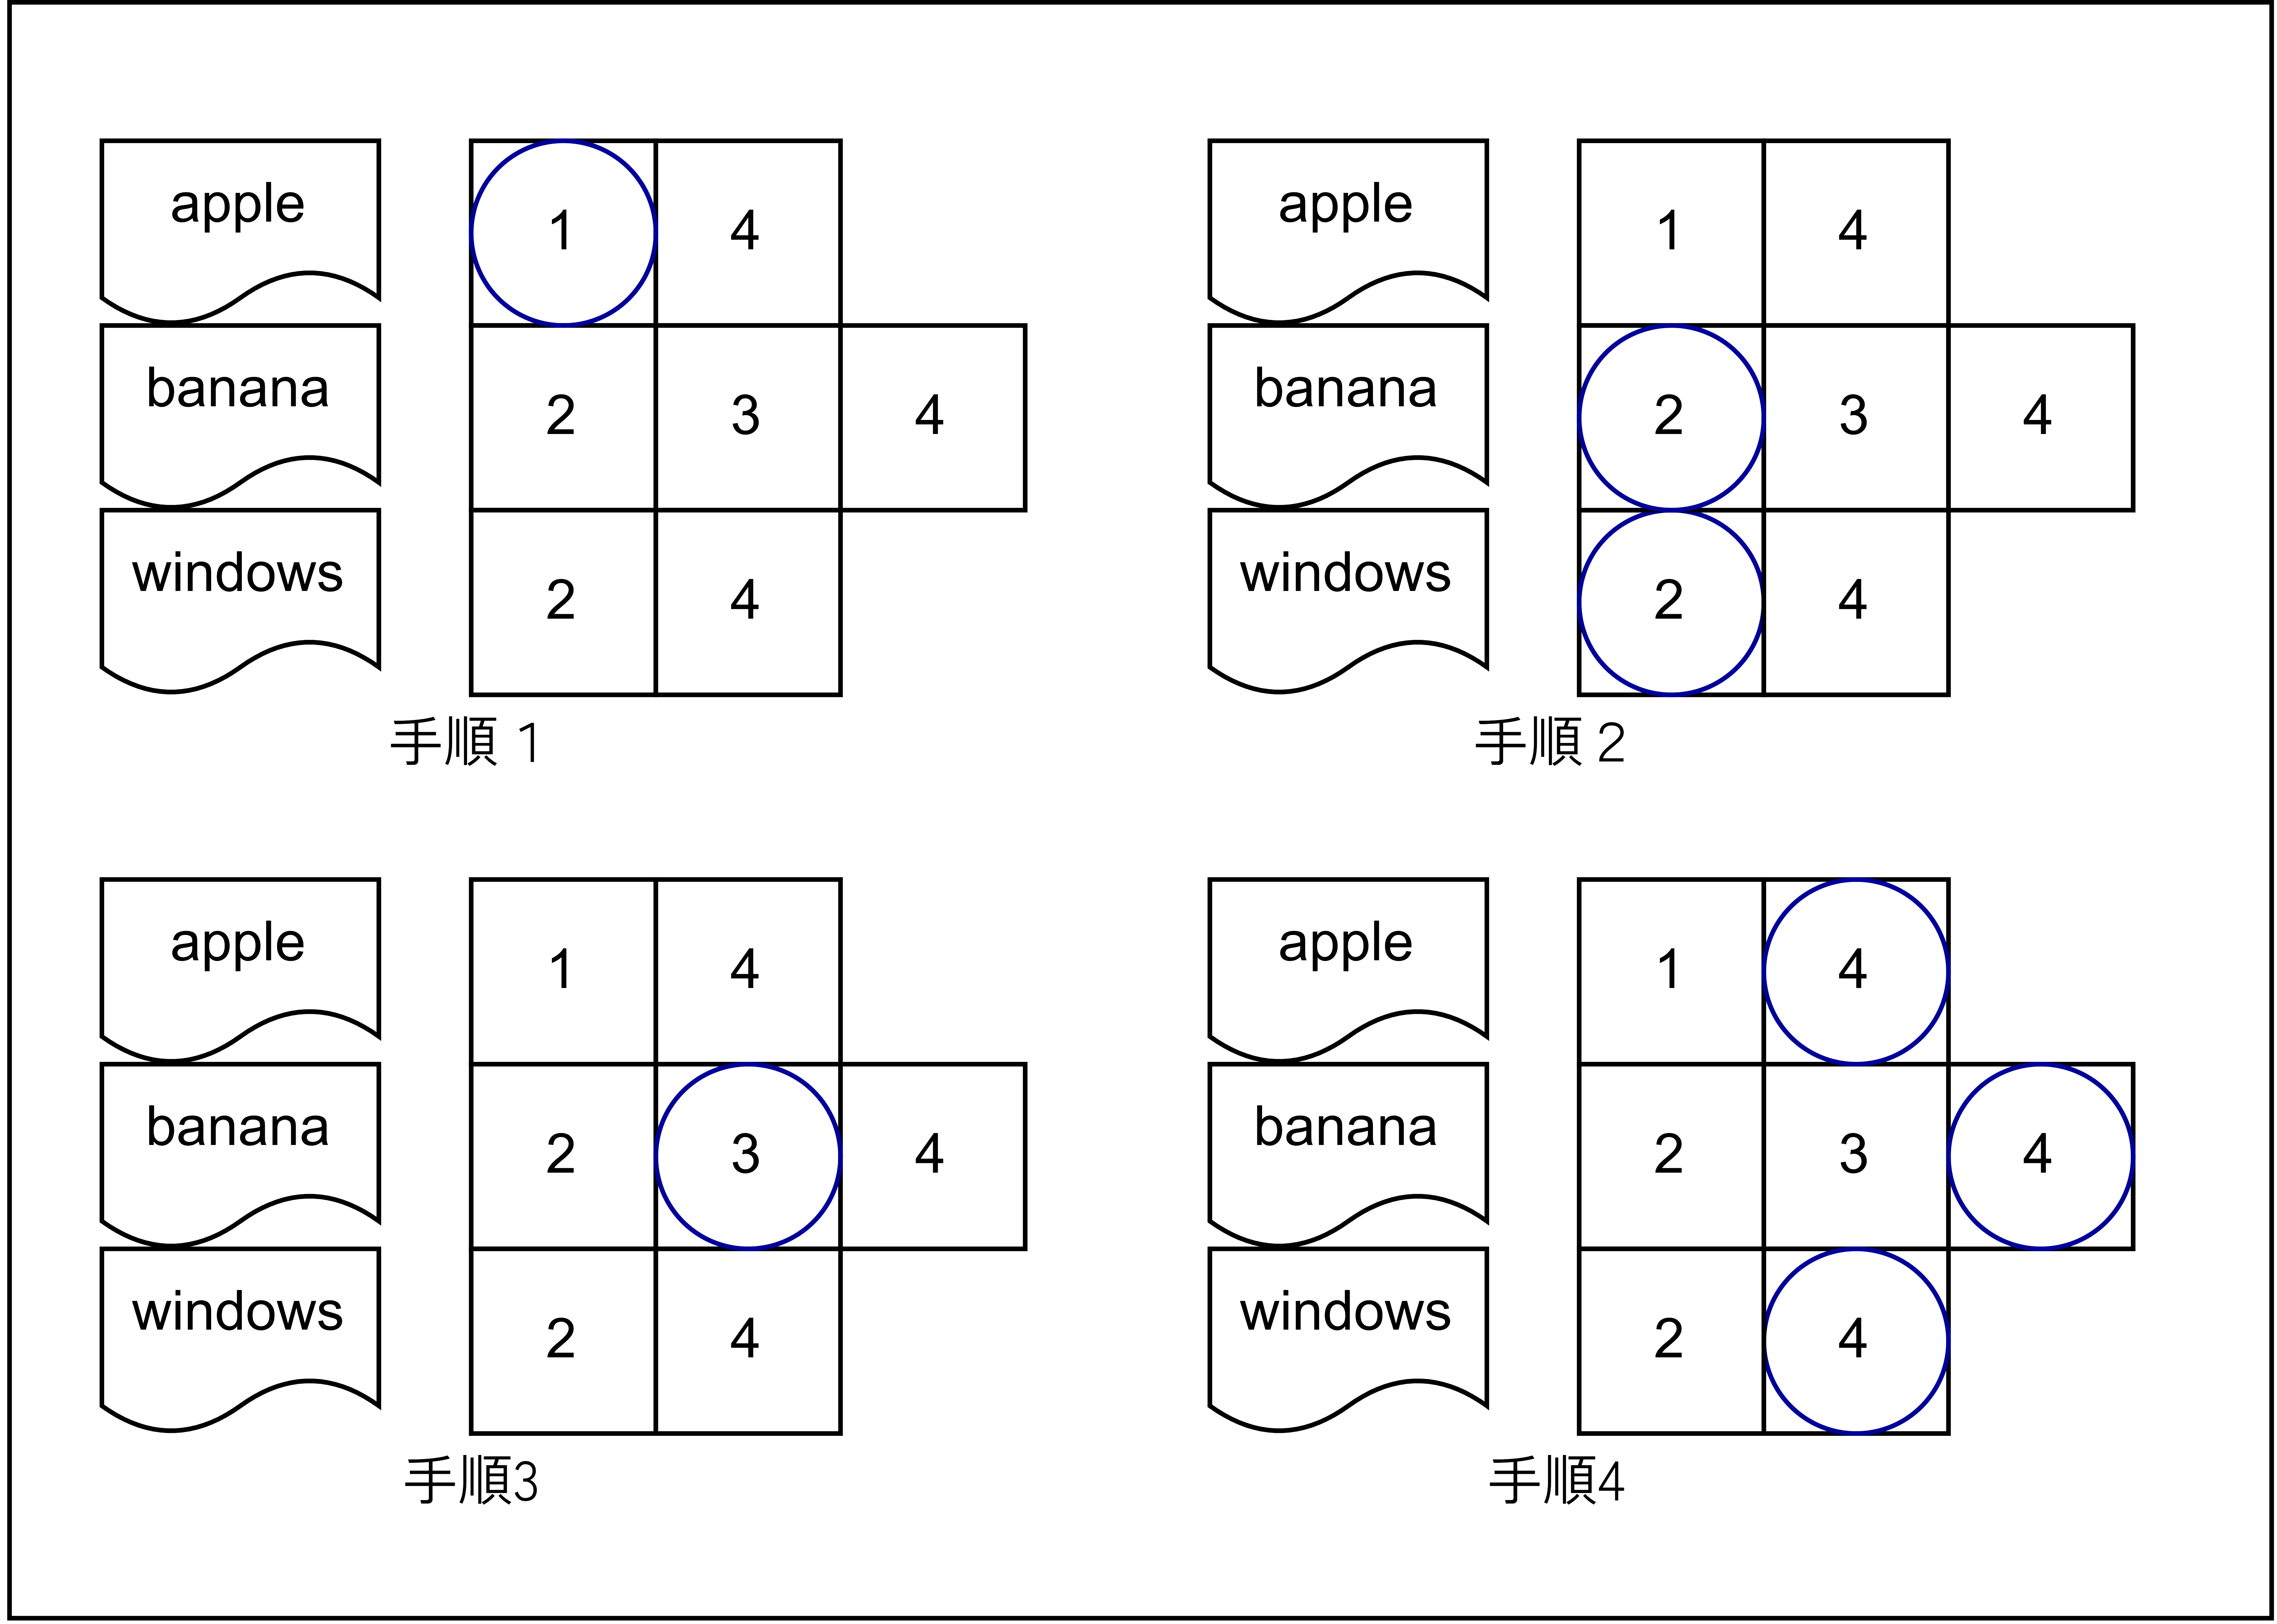
\includegraphics[width=8.7cm]{img/daat.png}
            \caption{DAATの手順}
            \label{fig:DAAT}
        \end{figure}
        
        %\item テキストに存在する単語に対応する集合に対して並列して処理を行う.転置インデクスのリストの中身がIDによって昇順や降順になっているとき,並列してリストの中身を走査することで同一テキストIDごとに処理を行うことができる.
    \end{description}
\end{itemize}
%エリとなるテキストがある場合,そのテキストに存在する単語についてひとつずつ転置インデクスを参照することで,#その単語がどのテキストに含まれているかをIDを通して高速に知ることができる.このとき,転置インデクスを用いた参照方法として主に2つの方法が存在し,その方法を今回の環境を用いて説明する.


\chapter{提案手法}
遅延評価法ではマッチング判定を行う際,クエリとデータベースにおいて共通する単語が1つもない場合でも,テキスト類似度を求めている.共通する単語が存在しない状況においてはテキスト類似度は0となり,マッチング判定対象に含める必要がない.よって,転置インデクスを用いて共通する単語が存在するテキストを抽出し,そのテキスト集合のみにマッチング判定処理を行うアルゴリズムを提案する.

\section{転置インデクスの管理}
\begin{comment}
静的なテキスト集合に対する転置インデクスは一度構築すれば更新する必要はない.しかし,本研究では動的なテキスト集合を扱うため,動的なテキスト集合に適した転置インデクスの構築・更新が必要になる.そのため,転置インデクスのデータ構造を以下の通りとする.
\begin{itemize}
    %\item 転置インデクスを単語をキーとしたハッシュテーブルを用いて表し,参照される先はキーとなる単語を含むテキストのIDを格納するキューを指す.
    \item 転置インデクスをハッシュテーブルとし,それぞれの単語にテキストIDを含むキューを対応させる.
    \item 新しいテキストが到着したとき,ハッシュテーブルを参照し,新しいテキストに含まれるすべての単語に対応するキューの先頭にテキスト情報を追加する.
    \item 最も古いテキストを除外するとき,ハッシュテーブルを参照し,古いテキストに含まれるすべての単語に対応するキューの末尾のテキスト情報を削除する.
\end{itemize}
\par
ひとつのテキスト内にある単語が複数含まれている時,その単語の個数分キューにテキストIDを追加するのではなく,テキストを識別するためのテキストIDとその単語の個数をもつデータをキューに格納することとし,このデータをテキスト情報とする.
\end{comment}

第\ref{chap:ii}章に従い,毎時刻テキストが到着し,スライディングウィンドウの内容が変化する度に転置インデクスを更新する.
%パターン1であればクエリに,パターン2であればデータベース上のすべてのユーザに転置インデクスを構築する必要がある.

\section{マッチング方向}
マッチング処理には以下で示す2つのパターンが存在する.
\begin{description}
    %\item \textbf{パターン1} データベース上のユーザのテキストがクエリユーザのどのテキストとマッチングするかの判定を行う(図\ref{fig:lazy}における$\mbox{OUT}_V$に対する処理,$\mbox{IN}_U$に対する処理)
    \item \textbf{パターン1} $U_T$内のテキスト$o \in U_T$を起点とするマッチング判定(図\ref{fig:lazy}における$\mbox{OUT}_V$に対する処理,$\mbox{IN}_U$に対する処理)
    %\item \textbf{パターン2} クエリユーザのテキストがデータベース上のユーザのどのテキストとマッチングするかの判定を行う(図\ref{fig:lazy}における最新の$V_{UM}$の頂点のマッチング判定)
    \item \textbf{パターン2} $V_T$内のテキスト$o \in V_T$を起点とするマッチング判定(図\ref{fig:lazy}における最新の$V_{UM}$の頂点のマッチング判定)
\end{description}

\subsection{LE-Q}
遅延評価法のパターン1の部分に対して転置インデクスを用いたマッチング判定を取り入れたアルゴリズムをLE-Q(Lazy Evaluation with inverted indices for Query)として提案する.このアルゴリズムを用いる場合,クエリ1人分のスライディングウィンドウに対する転置インデクスを管理する必要がある.LE-Qの$\mbox{OUT}_V$に対する処理,$\mbox{IN}_U$に対する処理における疑似コードをAlgorithm \ref{alg:LE-Q-1}, Algorithm \ref{alg:LE-Q-2}に示す.

\begin{algorithm}[H]
    \caption{LE-Q : $\mbox{OUT}_V$に対する処理}
    \label{alg:LE-Q-1}
    \begin{algorithmic}[1]
    \State $\mbox{OUT}_V$をスライディングウィンドウから離脱させる
    \If {$\mbox{OUT}_V\in V_{M}$}
        \State $O_U\leftarrow Pair(\mbox{OUT}_V)$
        \State $h \leftarrow PriorityQueue()$
        \For {$o \in O_U$}
            \State $h.add(InvertedIndexQuery[o])$
        \EndFor
        \While {$not\;h.empty()$}
            \State $O_V \leftarrow h.get()$
            \State $h.add(O_Vを格納する転置インデクスのリスト内の次のテキスト)$
            \If {$O_V \in V_{UM}$}
                \If {($jac(O_V,O_U)\geq \epsilon_{doc}$)}
                    \State $O_V$と$O_U$がマッチング
                    \State break
                \EndIf
            \EndIf
        \EndWhile
    \EndIf
    \end{algorithmic}
\end{algorithm}

\begin{algorithm}[H]
    \caption{LE-Q : $\mbox{IN}_U$に対する処理}
    \label{alg:LE-Q-2}
    \begin{algorithmic}[1]
    \State $h \leftarrow PriorityQueue()$
    \For {$o \in \mbox{IN}_U$}
        \State $h.add(InvertedIndexQuery[o])$
    \EndFor
    \While {$not\;h.empty()$}
        \State $O_V \leftarrow h.get()$
        \State $h.add(O_Vを格納する転置インデクスのリスト内の次のテキスト)$
        \If {$O_V \in V_{UM}$}
            \If {($jac(O_V,\mbox{IN}_U)\geq \epsilon_{doc}$)}
                \State $O_V$と$\mbox{IN}_U$がマッチング
                \State break
            \EndIf
        \EndIf
    \EndWhile
    \end{algorithmic}
\end{algorithm}

\subsection{LE-QD}
遅延評価法のパターン1,パターン2の部分に対して転置インデクスを用いたマッチング判定を取り入れたアルゴリズムをLE-QD(Lazy Evaluation with inverted indices for Query and Database)として提案する.このアルゴリズムを用いる場合,クエリ1人分に加えデータベース上のユーザ全員のスライディングウィンドウに対する転置インデクスを管理する必要がある.LE-QDの$\mbox{OUT}_V$に対する処理,$\mbox{IN}_U$に対する処理はAlgorithm \ref{alg:LE-Q-1},Algorithm \ref{alg:LE-Q-2}と同様である.
図\ref{fig:lazy}における最新の$V_{UM}$の頂点のマッチング判定における疑似コードをAlgorithm \ref{alg:LE-QD-3}に示す.

\begin{algorithm}[H]
    \caption{LE-QD : 最新の$V_{UM}$の頂点のマッチング判定}
    \label{alg:LE-QD-3}
    \begin{algorithmic}[1]
    \While {$|V_M| < \epsilon$ AND $|V_{NM}| \leq (w-\epsilon)$}
    \State $O_V \leftarrow V_{UM} $の一番新しいテキスト
      
    \State $h \leftarrow PriorityQueue()$
    \For {$o \in O_V$}
        \State $h.add(InvertedIndexDatabase[o])$
    \EndFor
    \While {$not\;h.empty()$}
        \State $O_U \leftarrow h.get()$
        \State $h.add(O_Uを格納する転置インデクスのリスト内の次のテキスト)$
        \If {$O_U \in U_{UM}$}
            \If {($jac(O_V,O_U)\geq \epsilon_{doc}$)}
                \State $O_V$と$O_U$がマッチング
                \State break
            \EndIf
        \EndIf
    \EndWhile
      
    \If{$O_V$がどの$U_{UM}$ともマッチングしない}
      \State $O_V\in V_{NM}$とする
    \EndIf
  \EndWhile
    \end{algorithmic}
\end{algorithm}

\section{マッチング判定方法}

マッチング判定を行う対象は新しいテキストから優先してマッチングすることが優位であることが遅延評価法で示されている.キューには到着した順に先頭からテキスト情報を格納しているため,マッチング判定は先頭からDAAT方式で参照していく.
判定の処理に関しては,どちらのパターンにおいても共通の処理を行い,そのマッチング判定方法を以下に示す.
\begin{enumerate}
    \item 調べるもとのテキスト$u_T$のそれぞれの単語$\{t_1, t_1, \cdots, t_{|u_T|}\}$に対応するリストを転置インデクスを用いて取得する.
    \item DAAT方式に則って取得したリストを先頭から新しいテキスト優先で並列に走査していく.
    \item 参照したテキストが
    \begin{itemize}
        \item パターン1では$V_{UM}$
        \item パターン2では$U_{UM}$
    \end{itemize}
    に含まれていれば以下の処理を行う.
    \item 同一IDをもつテキストごとに共通する単語がいくつ存在するかを数える.
    \item 異なるテキストIDが登場する,または最後のテキストを参照したときに,式(\ref{match})を用いてテキスト類似度を計算する.
    \item 式(\ref{match})の値が$\epsilon_{doc}$以上であればマッチング,そうでなければ非マッチングとする.
\end{enumerate}

\chapter{LE-Qの改善案}
LE-Qではデータベース側に転置インデクスを持たないため,パターン2の$V_T$を起点とするマッチング判定で転置インデクスを使用しない.

ここでユーザ間類似度$\mbox{sim}(V_T,U_T)$が$\epsilon_u$と近い時,パターン2の処理で$V_{UM}$の多くのテキストをマッチング判定
しないと類似,非類似を確定できない.つまり,枝刈りの効果が期待できない.このように枝刈りの効果が弱い場合に,$V_{UM}$に
属するテキストを起点とする転置インデクスを使わないマッチング判定を,$U_{UM}$に属するテキストを起点としてクエリ側の転置インデクス
を使用するマッチング判定に切り替える改善案を提案する.具体的には$\epsilon_r$を閾値パラメータとして,以下の基準でマッチング判定
モードを切り替える.
\begin{itemize}
\item モード1: $|V_{UM}|< \epsilon_r$ならば,$U_{UM}$に属するテキストを起点としてマッチング判定
\item モード2: $|V_{UM}|\ge \epsilon_r$ならば,$V_{UM}$に属するテキストを起点としてマッチング判定
\end{itemize}

モード1の$U_{UM}$に属するテキストを起点とするマッチング判定処理を以下に述べる.$\forall O_U \in U_{UM}$に対してマッチング判定を
行っており,極大マッチングを完成させる点に注意されたい.
\begin{quote}
    %\item $U_{UM}$からひとつずつテキストを\textbf{すべて}取り出し,$V_{UM}$のどのテキストとマッチングするかの判定を行う.
\noindent {\bf Step 1:} $\forall O_U \in U_{UM}$を起点とし, $V_{UM}$内のテキストを対象としたマッチング判定を転置インデクスを用いて行う.
その結果, $O_U$と$V_{UM}$のテキスト$O_V$がマッチングした時,$O_U \in U_M,O_V \in V_M$とする.\\
\noindent {\bf Step 2:} $U_{UM}$の全テキストのマッチング判定後,$V_{UM}$に残っているテキストをすべて$V_{NM}$に分類する.
\end{quote}

以上をまとめると.$|V_{UM}|$が小さく枝刈りが期待できない状況では遅延評価をせずに,モード1で転置インデクスを使って高速に極大マッチングを完成させるということになる.これを$\epsilon_r$を用いたマッチング切替と呼ぶ.

一方で,$|V_{UM}|$が極端に小さい時,転置インデクスを用いたマッチング判定が転置インデクスを用いないマッチング判定よりも遅い場合があると考える.

$U_{UM}$に属するテキストを起点とした転置インデクスを用いるマッチング判定では,
\begin{enumerate}
    \item テキストに含まれるそれぞれの単語の転置リストを取得
    \item DAAT方式でテキストを走査
\end{enumerate}
を行う.転置インデクスはクエリユーザの全テキストにより構成されるため,$V_M, V_{NM}, V_{UM}$所属のテキストが混在する.
%よってマッチング判定を行う際,
よってマッチング判定を行う際,パターン2において
\begin{itemize}
    %\item パターン1 : マッチング相手が$V_{NM}$所属であること
    %\item パターン2 : マッチング相手が$V_{UM}$所属であること
    \item マッチング相手が$V_{UM}$所属であること
\end{itemize}
を満たすテキストにのみマッチング判定をする必要がある.このことから$V_{UM}$に属するテキストが少ないとき,転置インデクスを参照しても$V_{UM}$に属さないテキストが取り出され,マッチング判定となる$V_{UM}$に属するテキストとなかなか遭遇しない.
%目的のテキスト集合に所属するテキストを見つけるまでに,それ以外のテキスト集合に所属するテキストを多く調べる必要があると考えられる.
この場合,マッチング判定は高速に行えるが$V_{UM}$に所属するテキストを見つけることに多くの時間がかかり,結果的に転置インデクスを用いないマッチングの方が早いと考える.よって$V_{UM}$の大きさが閾値$\epsilon_m$以下のとき,マッチング方法を転置インデクスを用いないマッチングに変更する.これを$\epsilon_m$を用いたマッチング切替と呼ぶ.

このように,遅延評価を実施するかを適応的に切り替えることから,LE-Qに$\epsilon_r$を用いたマッチング切替と$\epsilon_m$を用いたマッチング切替を取り入れたアルゴリズムをALE-Q (Adaptive LE-Q)と名付ける.

\chapter{実験}
従来手法となる遅延評価法,本稿で提案したLE-Q,LE-QD,ALE-Qの性能を比較する評価実験を行った.
各実験において,
\begin{enumerate}
    \item 実行時間
    \item マッチング判定回数
\end{enumerate}
の比較を行う.また,実験を行う環境として,
Intel(R) Core(TM) i7-6700 CPU @3.40GHz,16GBメモリ,Ubuntu20.04
を用意した.
各実験において以下の設定を用いる.
\begin{itemize}
    \item スライディングウィンドウの大きさ 100
    \item シミュレートする時刻 1から1000
    \item テキスト類似度の閾値$\epsilon_{doc}$を0.1
    \item ユーザ間類似度の閾値$\epsilon_u$を0,10,20,30,40,50,60,70,80,90,100と変化させた.
\end{itemize}

\section{人工データセット}
人工データセットを以下のルールに則って生成した.全ユーザは3単語で構成されるテキストを1000個ずつ持つ.単語集合$\Phi_q,\Phi_{nq}$を用意し,
\begin{itemize}
    \item $\Phi_q \cap \Phi_{nq} = \phi$
    \item $|\Phi_q|=1000$
    \item $|\Phi_{nq}|=1000$
\end{itemize}
とする.
\begin{itemize}
    \item クエリユーザのテキストは$\Phi_q$から重複ありでランダムに選んだ単語で構成する.
    \item データベース側にはユーザを100人用意する.
    $i$番目($1\le i \le 100$)のユーザの時刻$t(1\le t\le 1000)$のテキストは,
    \begin{itemize}
        %\item $0.96^{(i-1)}$の確率で$t-100 \le t' < t+100$を満たす$t'$をランダムに決定し,クエリの時刻$t'$のテキストとする.
        \item $p$の確率で$t-100 \le t' < t+100$を満たす$t'$をランダムに決定し,クエリの時刻$t'$のテキストとする.
        %\item $1-0.96^{(i-1)}$の確率で$\Phi_{nq}$から重複を許してランダムに選んだ単語とする.
        \item $1-p$の確率で$\Phi_{nq}$から重複を許してランダムに選んだ単語とする.
    \end{itemize}
\end{itemize}
以上の条件をもとに以下の6つのデータセットを作成する.
\begin{enumerate}
    \item $p=0.1$としたときのデータセット
    \item $p=0.3$としたときのデータセット
    \item $p=0.5$としたときのデータセット
    \item $p=0.7$としたときのデータセット
    \item $p=0.9$としたときのデータセット
    \item $p=0.96^{(i-1)}$としたときのデータセット
    \begin{itemize}
        \item $i$が小さいほどクエリユーザのテキストを選ぶ確率が大きくなるため,$i$が大きいユーザほど,クエリユーザとの類似度の期待値が小さくなる.
    \end{itemize}
\end{enumerate}
これらのデータセットを用いて,各時刻に1つのテキストが到着する環境をシミュレートする.

\section{CoPhIRデータセット}
実データとしてFlickrアーカイブからメタデータを抽出したCoPhIR(Content-based Photo Image Retrieval)\cite{CoPhIR}\cite{2009}データセットを用いる.
このデータセットの各エントリには以下の内容が含まれている.
\begin{itemize}
    \item Flickr Webサイトの対応するエントリへのリンク
    \item 写真画像のサムネイル
    \item 対応するFlickrエントリ内のFlickrユーザ情報を含むXML構造体
    \begin{itemize}
        \item タイトル
        \item 位置
        \item GPS
        \item タグ
        \item コメント
    \end{itemize}
    \item 5つの標準MPEG-7画像特徴を抽出したXML構造体
    \begin{itemize}
        \item Scalable Colour
        \item Colour Structure
        \item Colour Layout
        \item Edge Histogram
        \item Homogeneous Texture
    \end{itemize}
\end{itemize}


CoPhIRデータセットに含まれる写真のメタデータから写真につけられたタグを単語とみなし,写真1枚に対して1つのテキストとし,本実験に適用した.なお,データセットは9108種類のタグと,100人のユーザから構成される.

ユーザごとに持つ写真の数は異なるが,すべて100個以上であるため,スライディングウィンドウの大きさ以上のテキストを持つ.テキストの数が1000に満たないユーザは古い時刻のテキストから順番に複製し,全ユーザが1000個のテキストを持つデータセットとする.


\section{転置インデクスの性能評価}
\label{exp1}
遅延評価法,LE-Q,LE-QDのアルゴリズムを人工データセット,CoPhIRデータセットを利用し,全ユーザの類似性を各時刻すべてにおいて求める実験を行った.
人工データセットにおける実験結果を図\ref{fig:exp1_art}に示す.
結果よりLE-QはLE-QDよりも高速に動作することが分かった.LE-QDはマッチング比較回数をかなり抑えることができたものの,転置インデクスの構築に時間がかかってしまい,結果的にLE-Qよりも多くの実行時間を要することとなったと考えられる.

\begin{figure}[H]
    \centering
    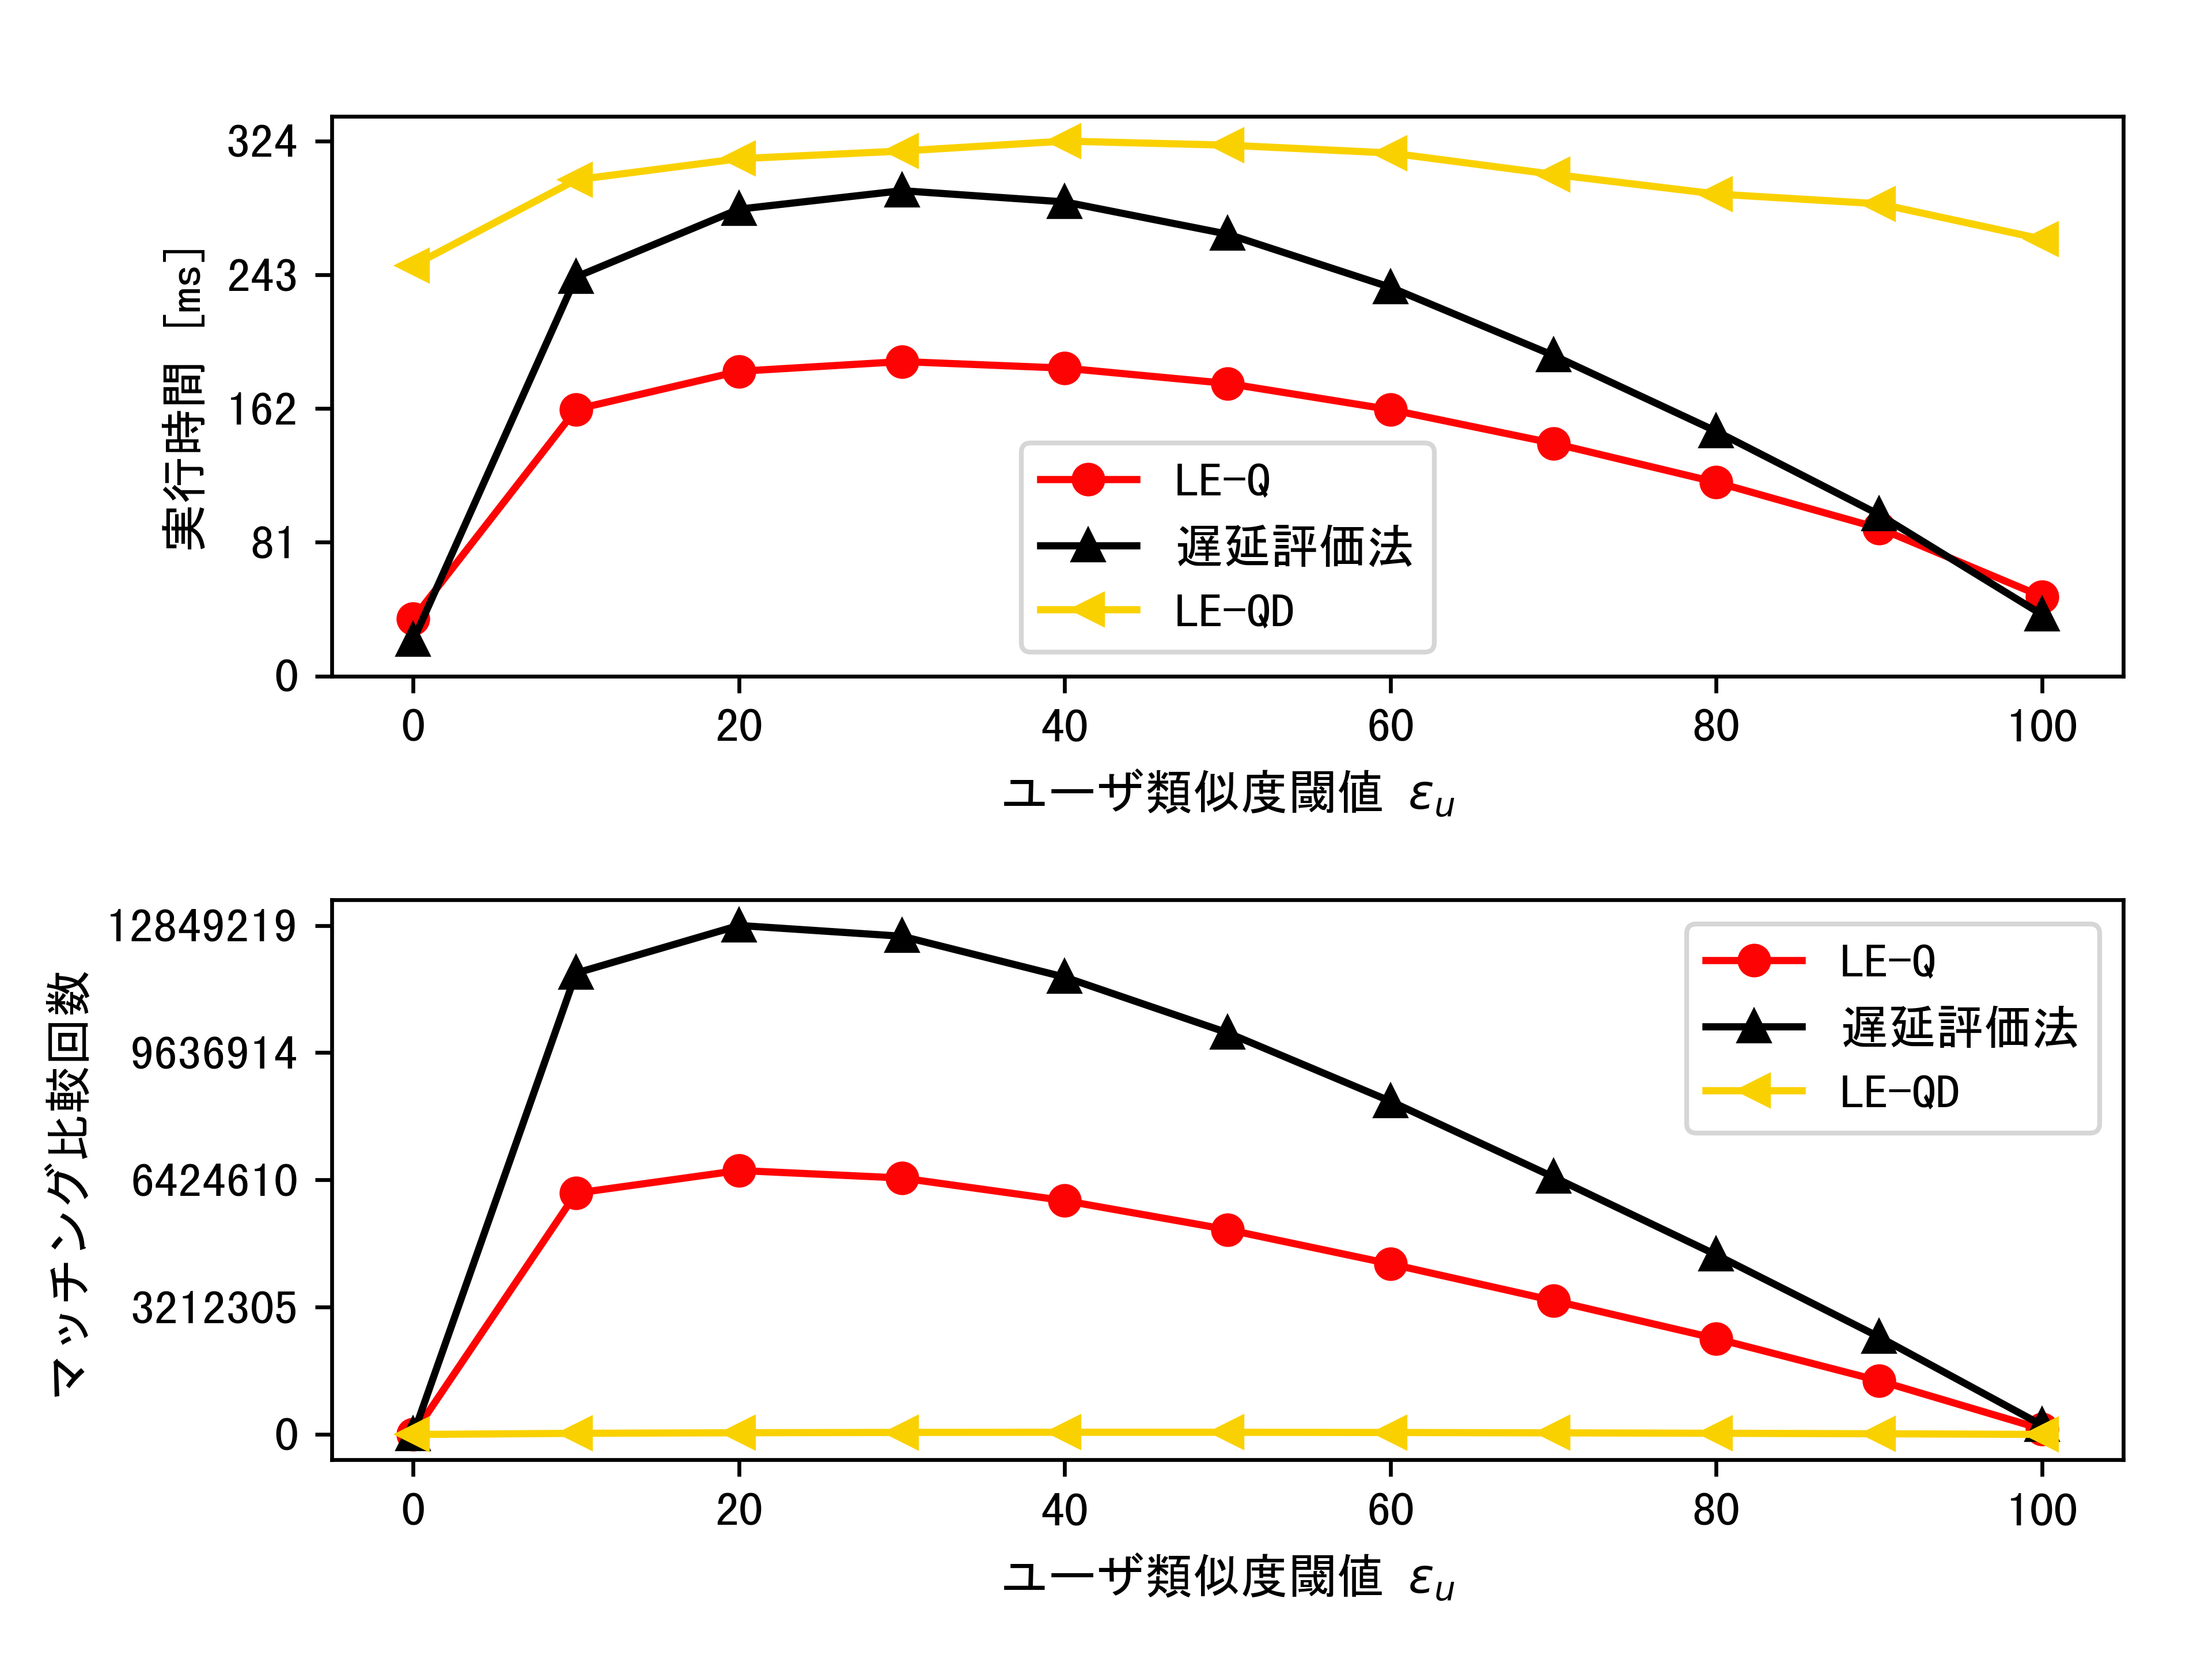
\includegraphics[width=8.3cm]{eimg/exp1.png}
    \caption{性能評価(人工データセット($p=0.96^{(i-1)}$))}
    \label{fig:exp1_art}
\end{figure}
CoPhIRデータセットにおける実験結果を図\ref{fig:exp1_cop}に示した.
%SNSのような現実世界の環境では,クエリユーザに対するデータベースユーザの類似度はほとんどの場合において小さくなると考えられる.そのため,実データのCoPhIRデータセットではLE-Qの方が優位である結果が得られたと考えられる.
図\ref{fig:exp1_art}と同様な結果を示し,LE-QDと遅延評価法よりLE-Qが効率的であると言える.

\begin{figure}[H]
    \centering
    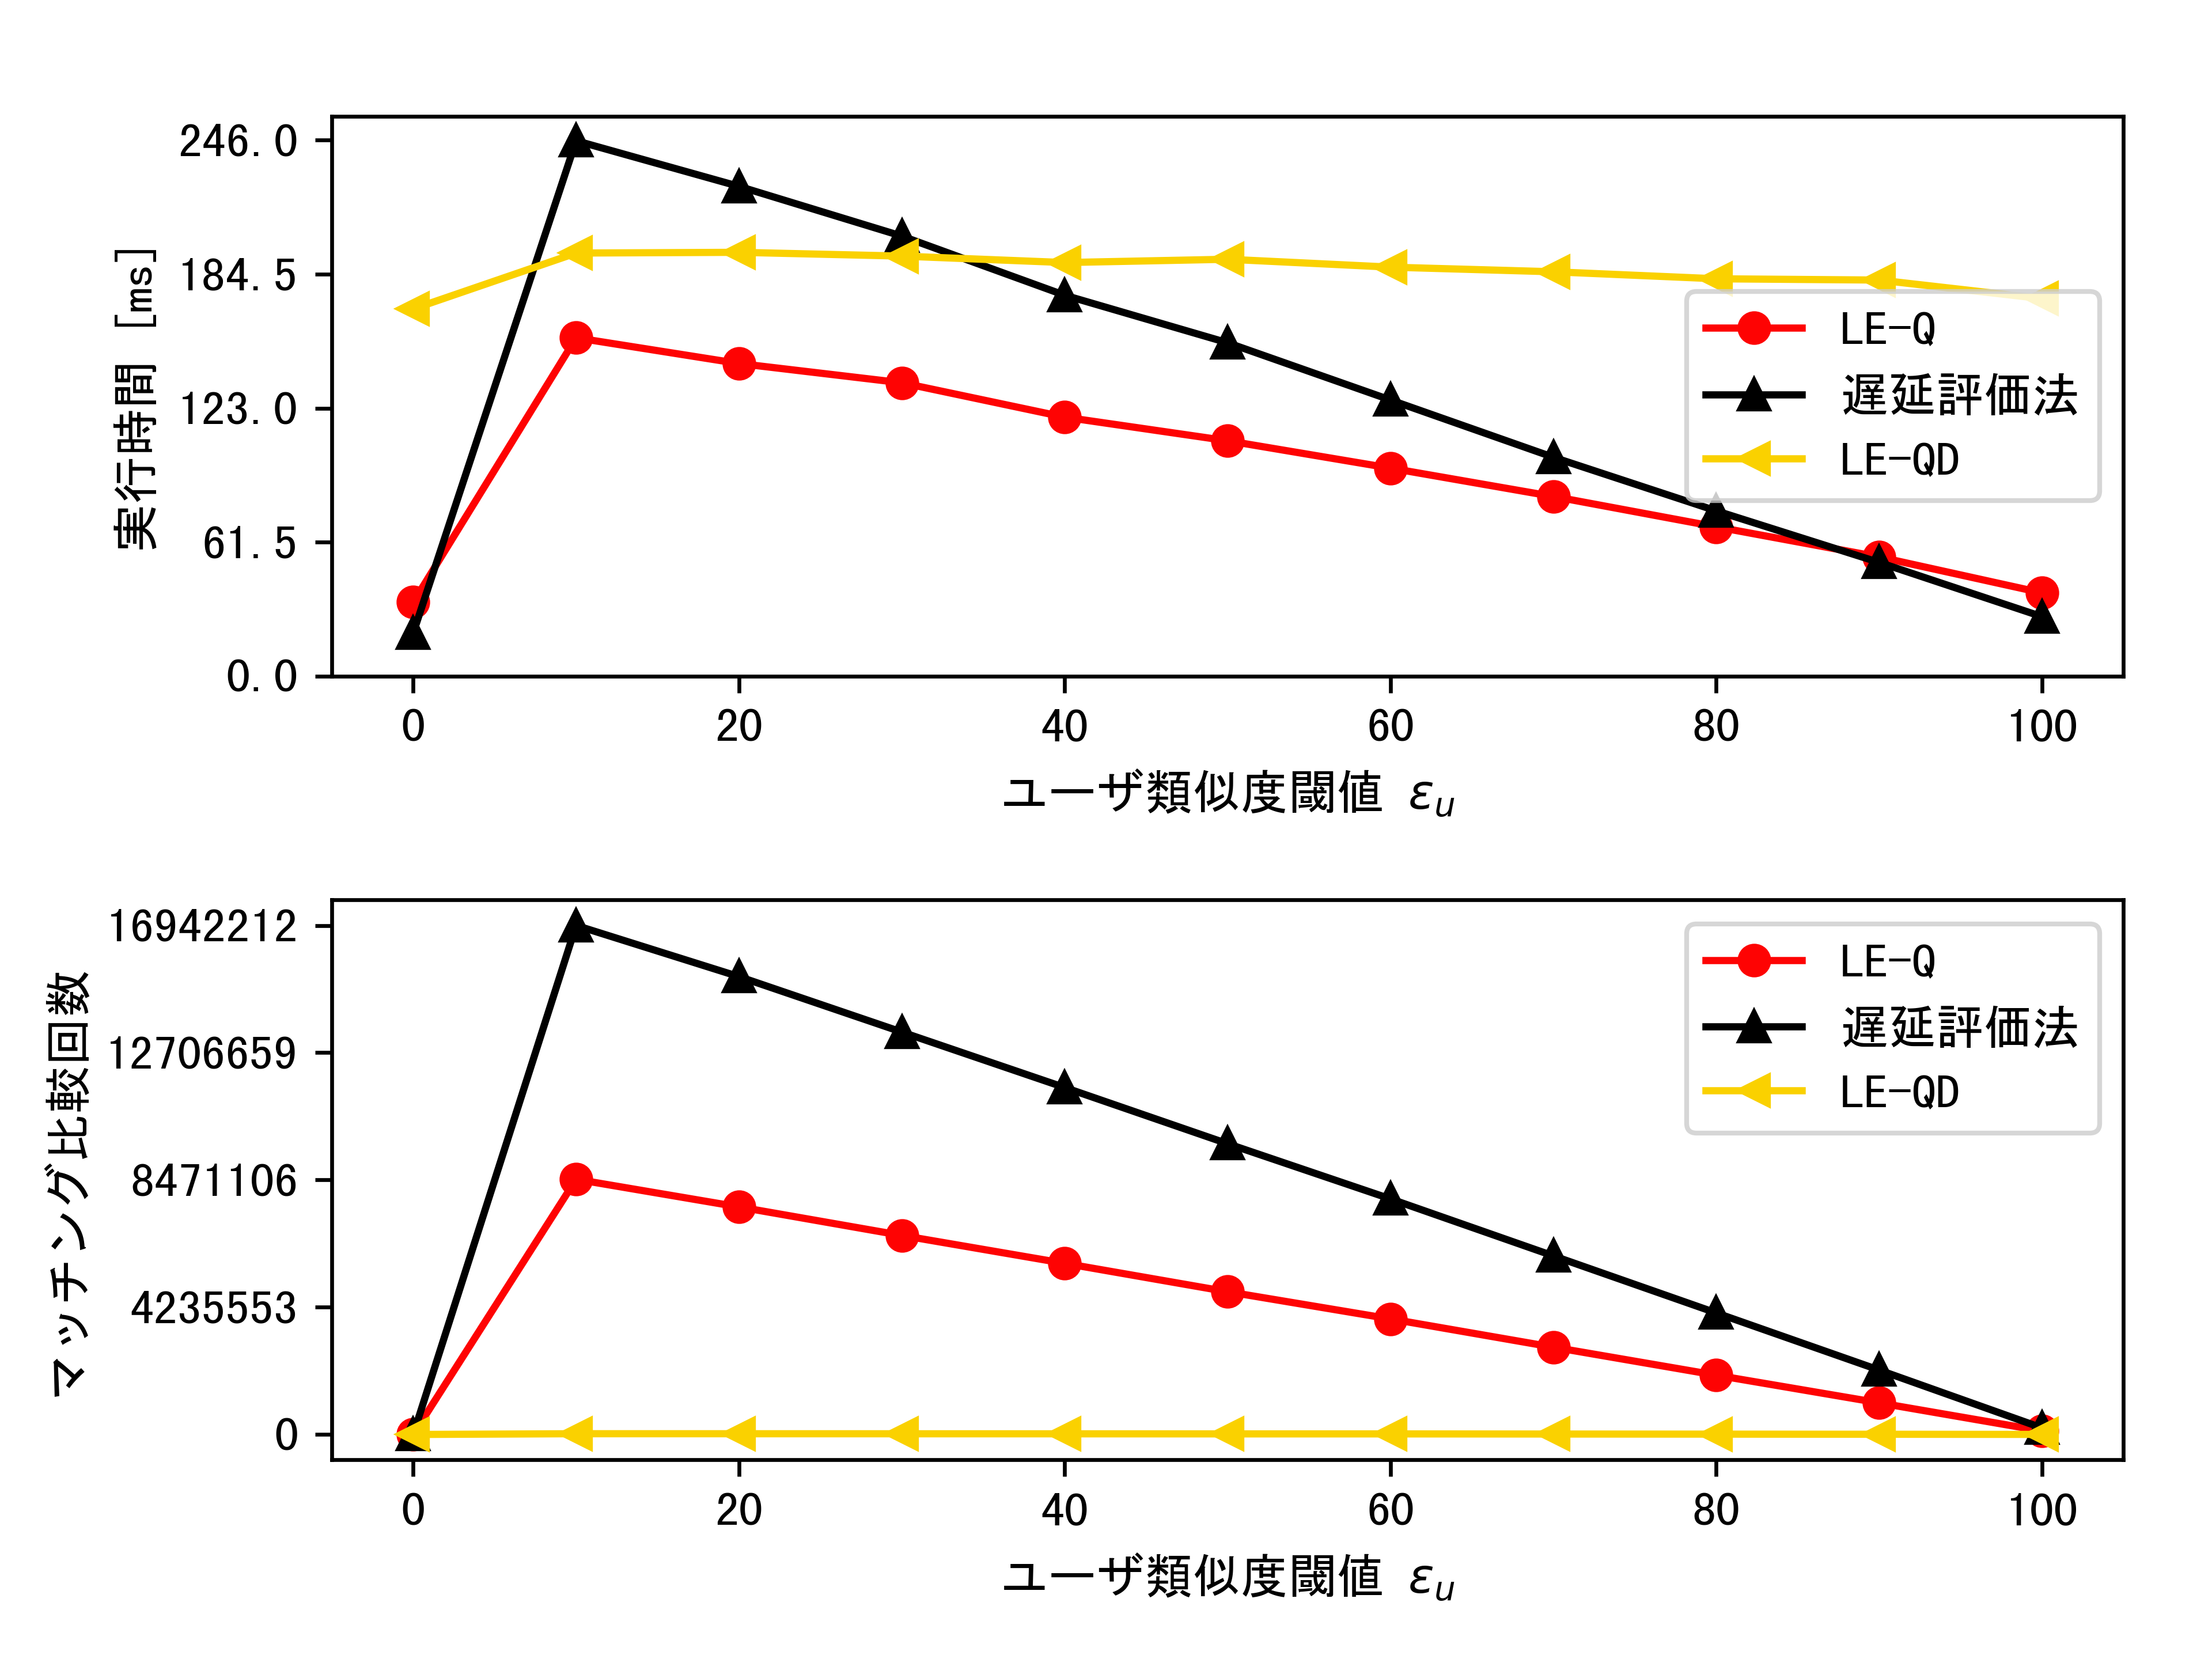
\includegraphics[width=8.3cm]{eimg/exp1_c.png}
    \caption{性能評価(CoPhIRデータセット)}
    \label{fig:exp1_cop}
\end{figure}

人工データセットにおける$p$を固定した場合の実験結果を図\ref{fig:exp1_art_1},図\ref{fig:exp1_art_3},図\ref{fig:exp1_art_5},図\ref{fig:exp1_art_7},図\ref{fig:exp1_art_9}に示した.
%クエリに対するデータベースユーザの類似度が小さい時には遅延評価法よりLE-Qの方が高速であるが,類似度が大きくなるに連れて,LE-Qより遅延評価法の方が高速に動作するような結果になった.
$p$の値によらず,LE-Qが最も効率的に動作していることがわかる.

\begin{figure}[H]
    \centering
    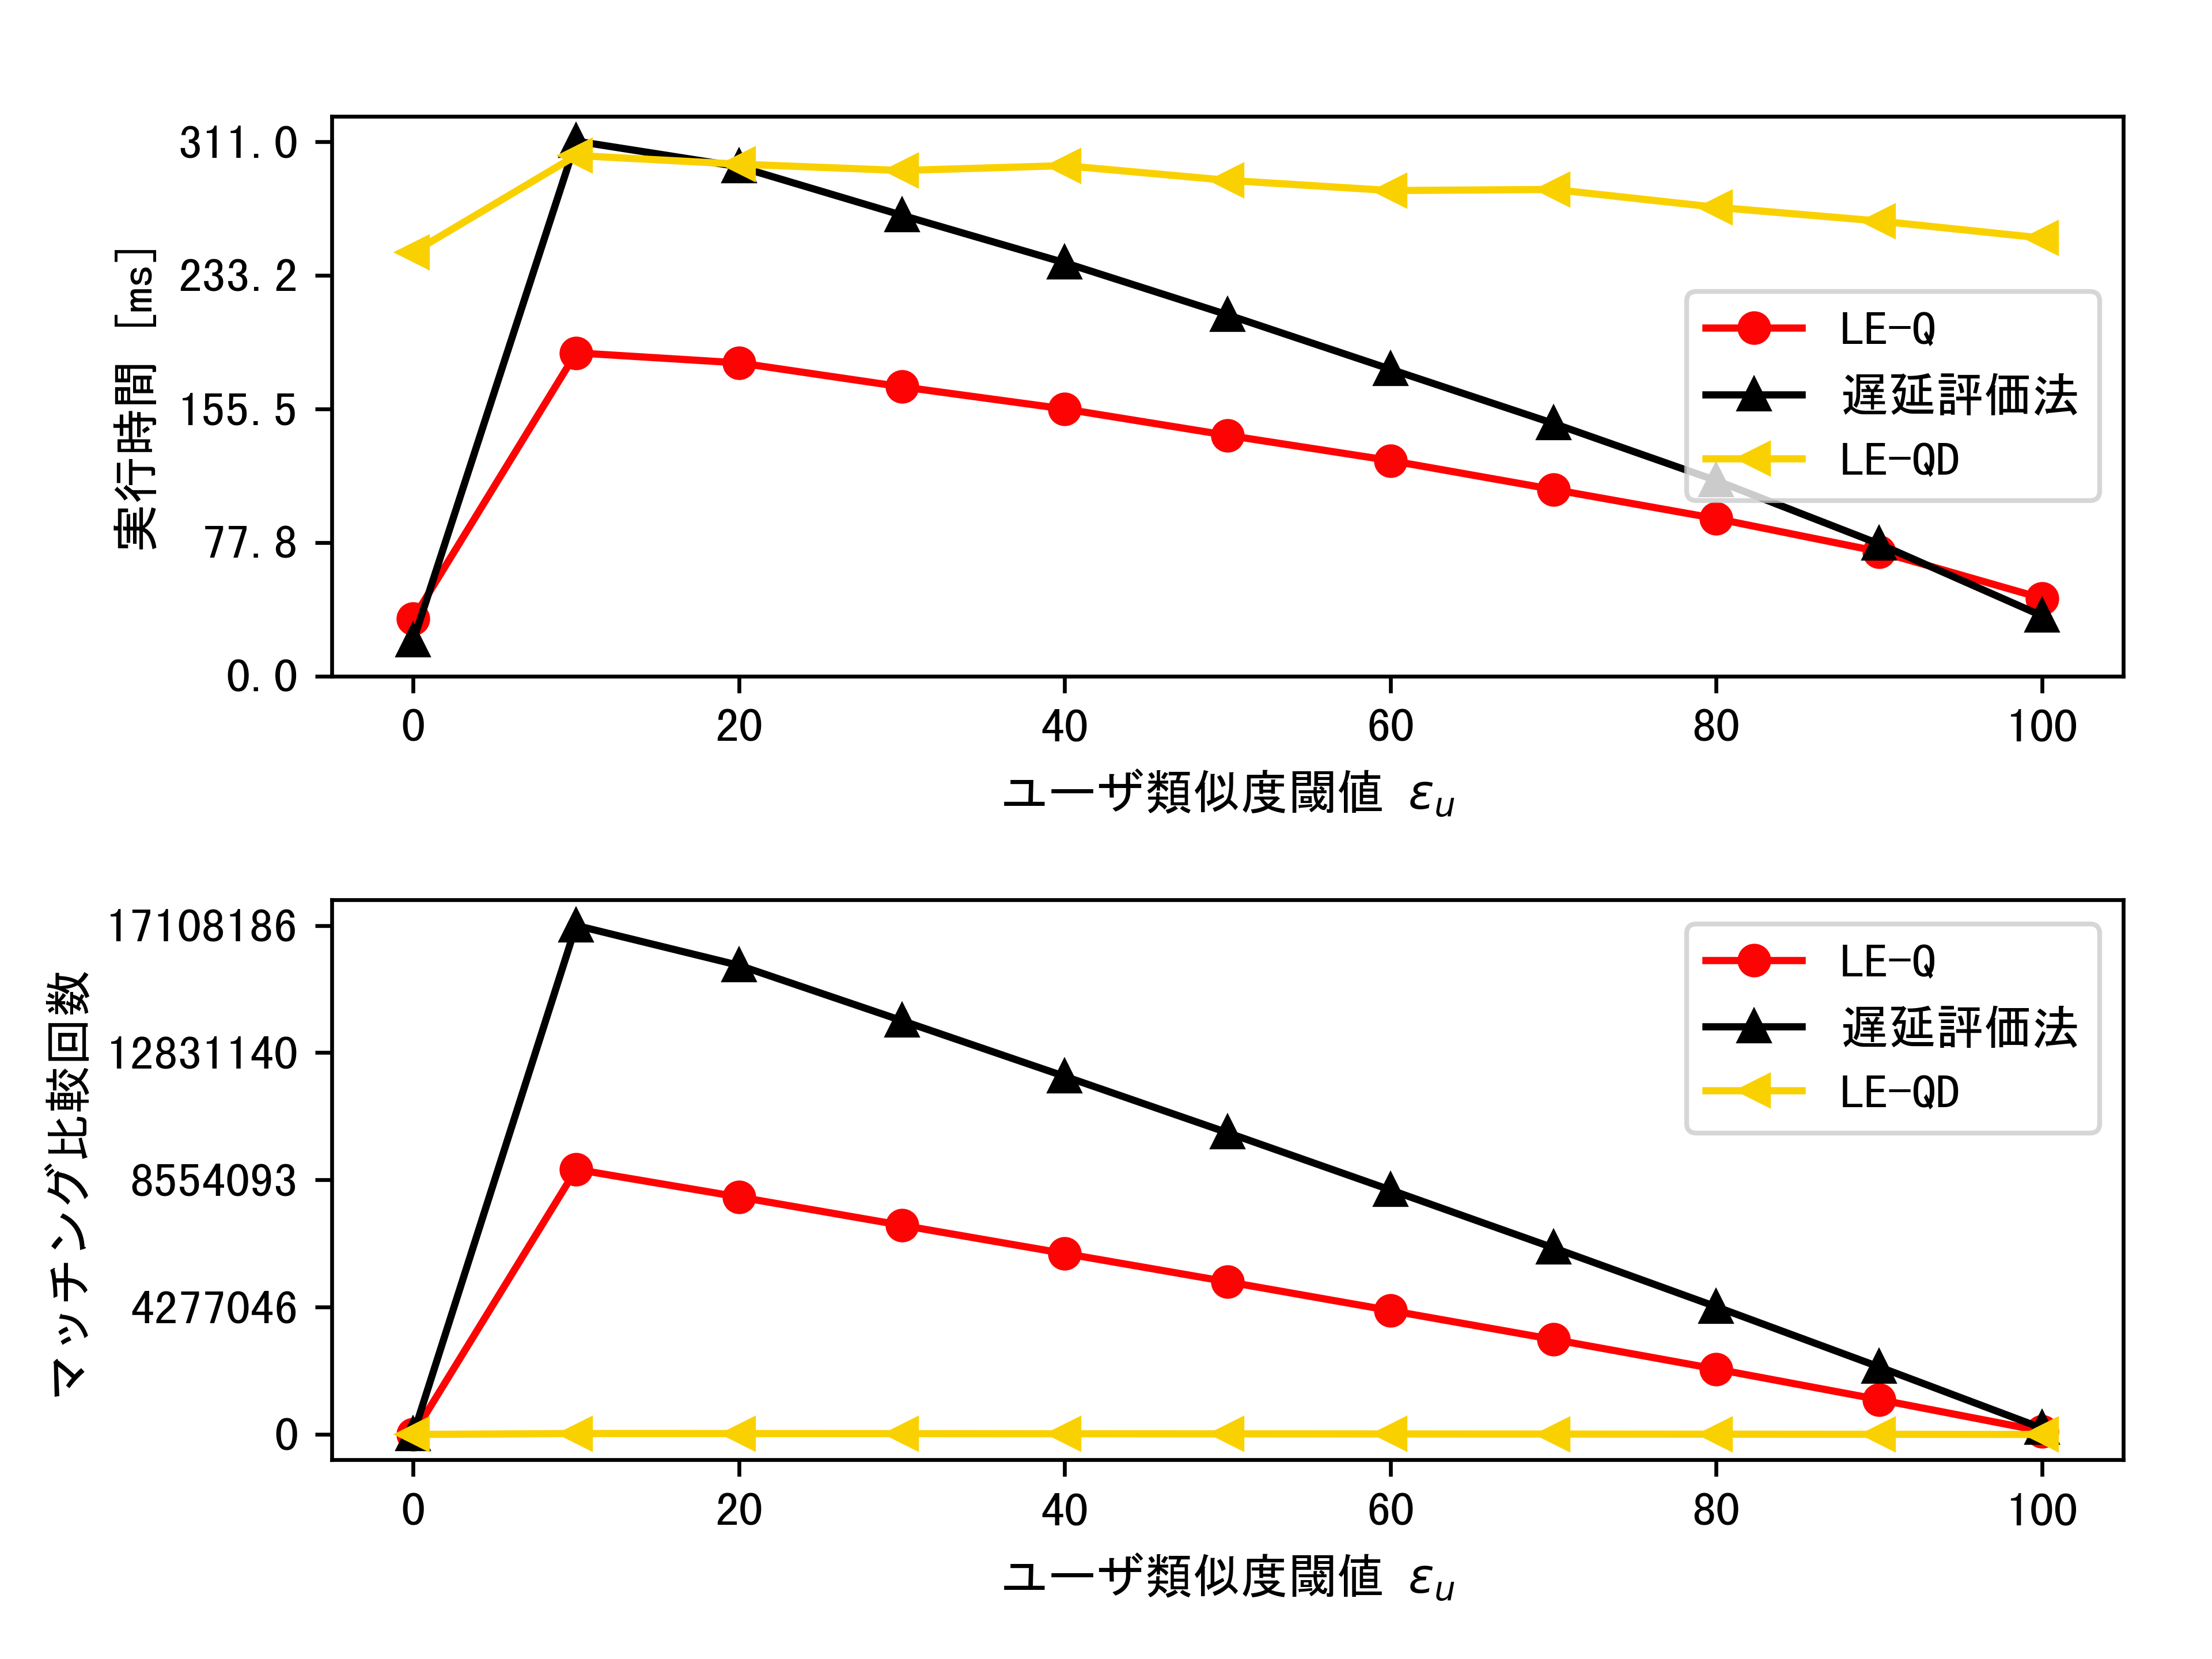
\includegraphics[width=8.3cm]{eimg/exp1_1.png}
    \caption{性能評価(人工データセット($p=0.1$))}
    \label{fig:exp1_art_1}
\end{figure}
\begin{figure}[H]
    \centering
    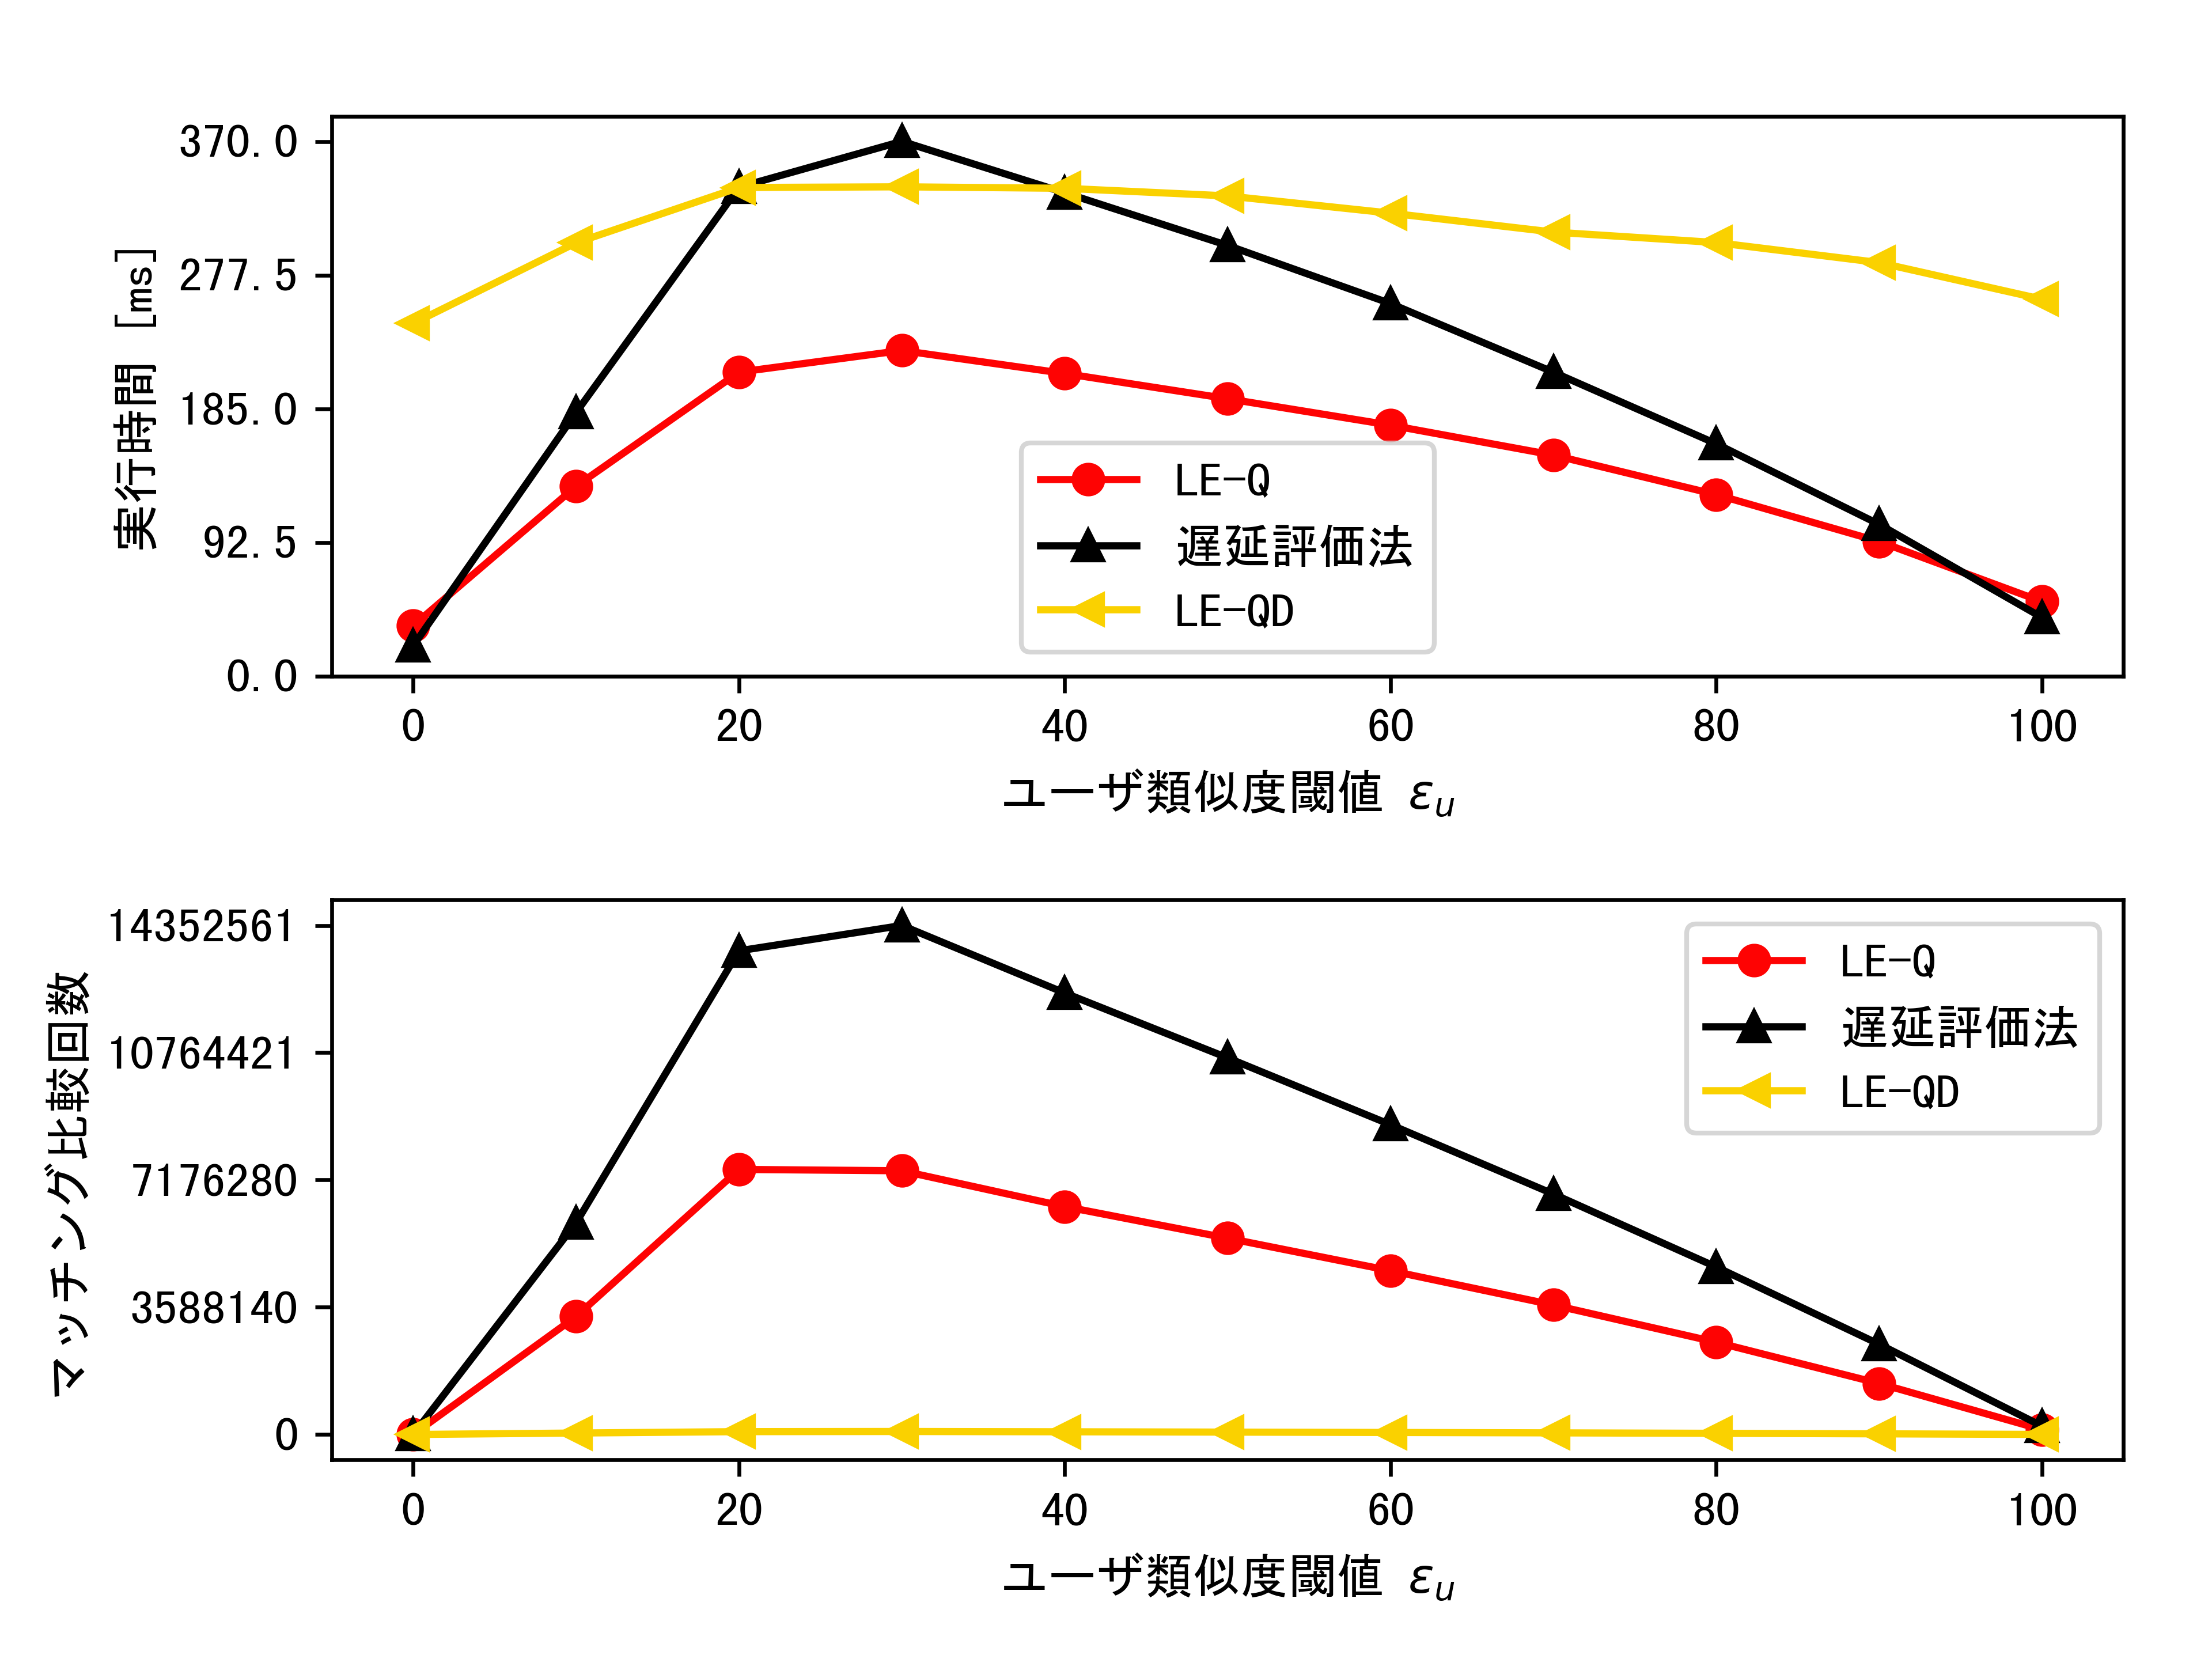
\includegraphics[width=8.3cm]{eimg/exp1_3.png}
    \caption{性能評価(人工データセット($p=0.3$))}
    \label{fig:exp1_art_3}
\end{figure}
\begin{figure}[H]
    \centering
    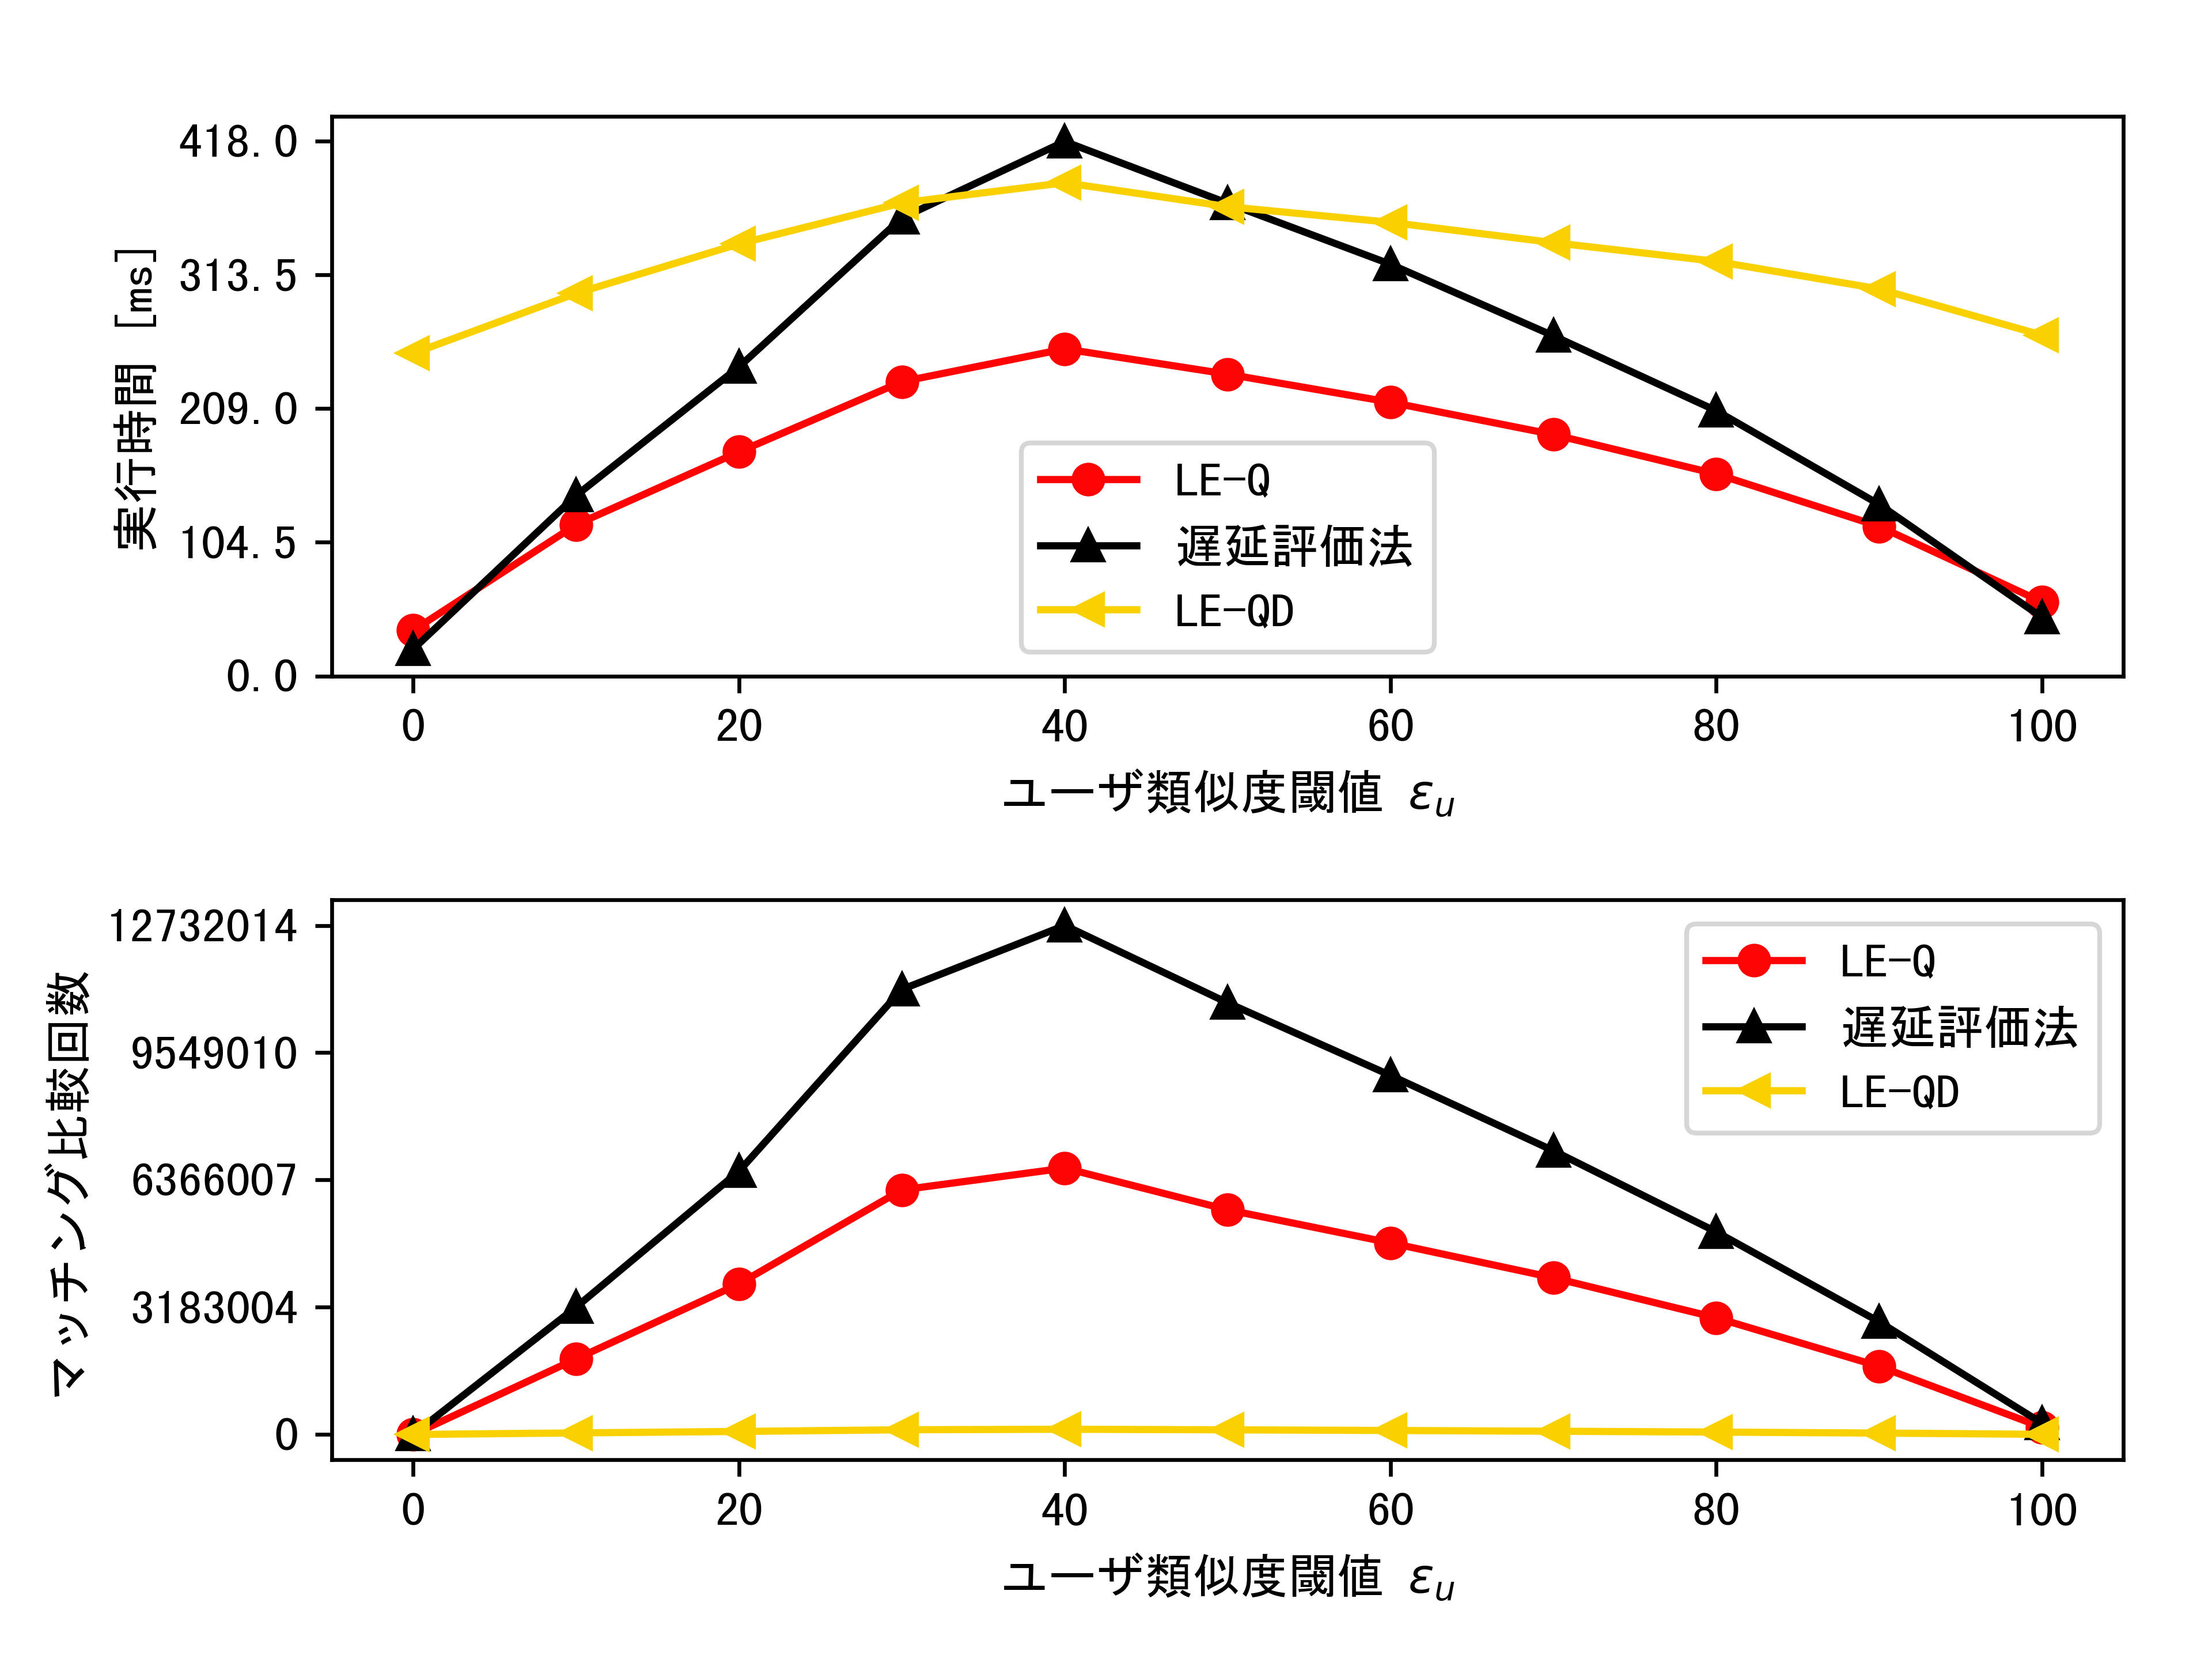
\includegraphics[width=8.3cm]{eimg/exp1_5.png}
    \caption{性能評価(人工データセット($p=0.5$))}
    \label{fig:exp1_art_5}
\end{figure}
\begin{figure}[H]
    \centering
    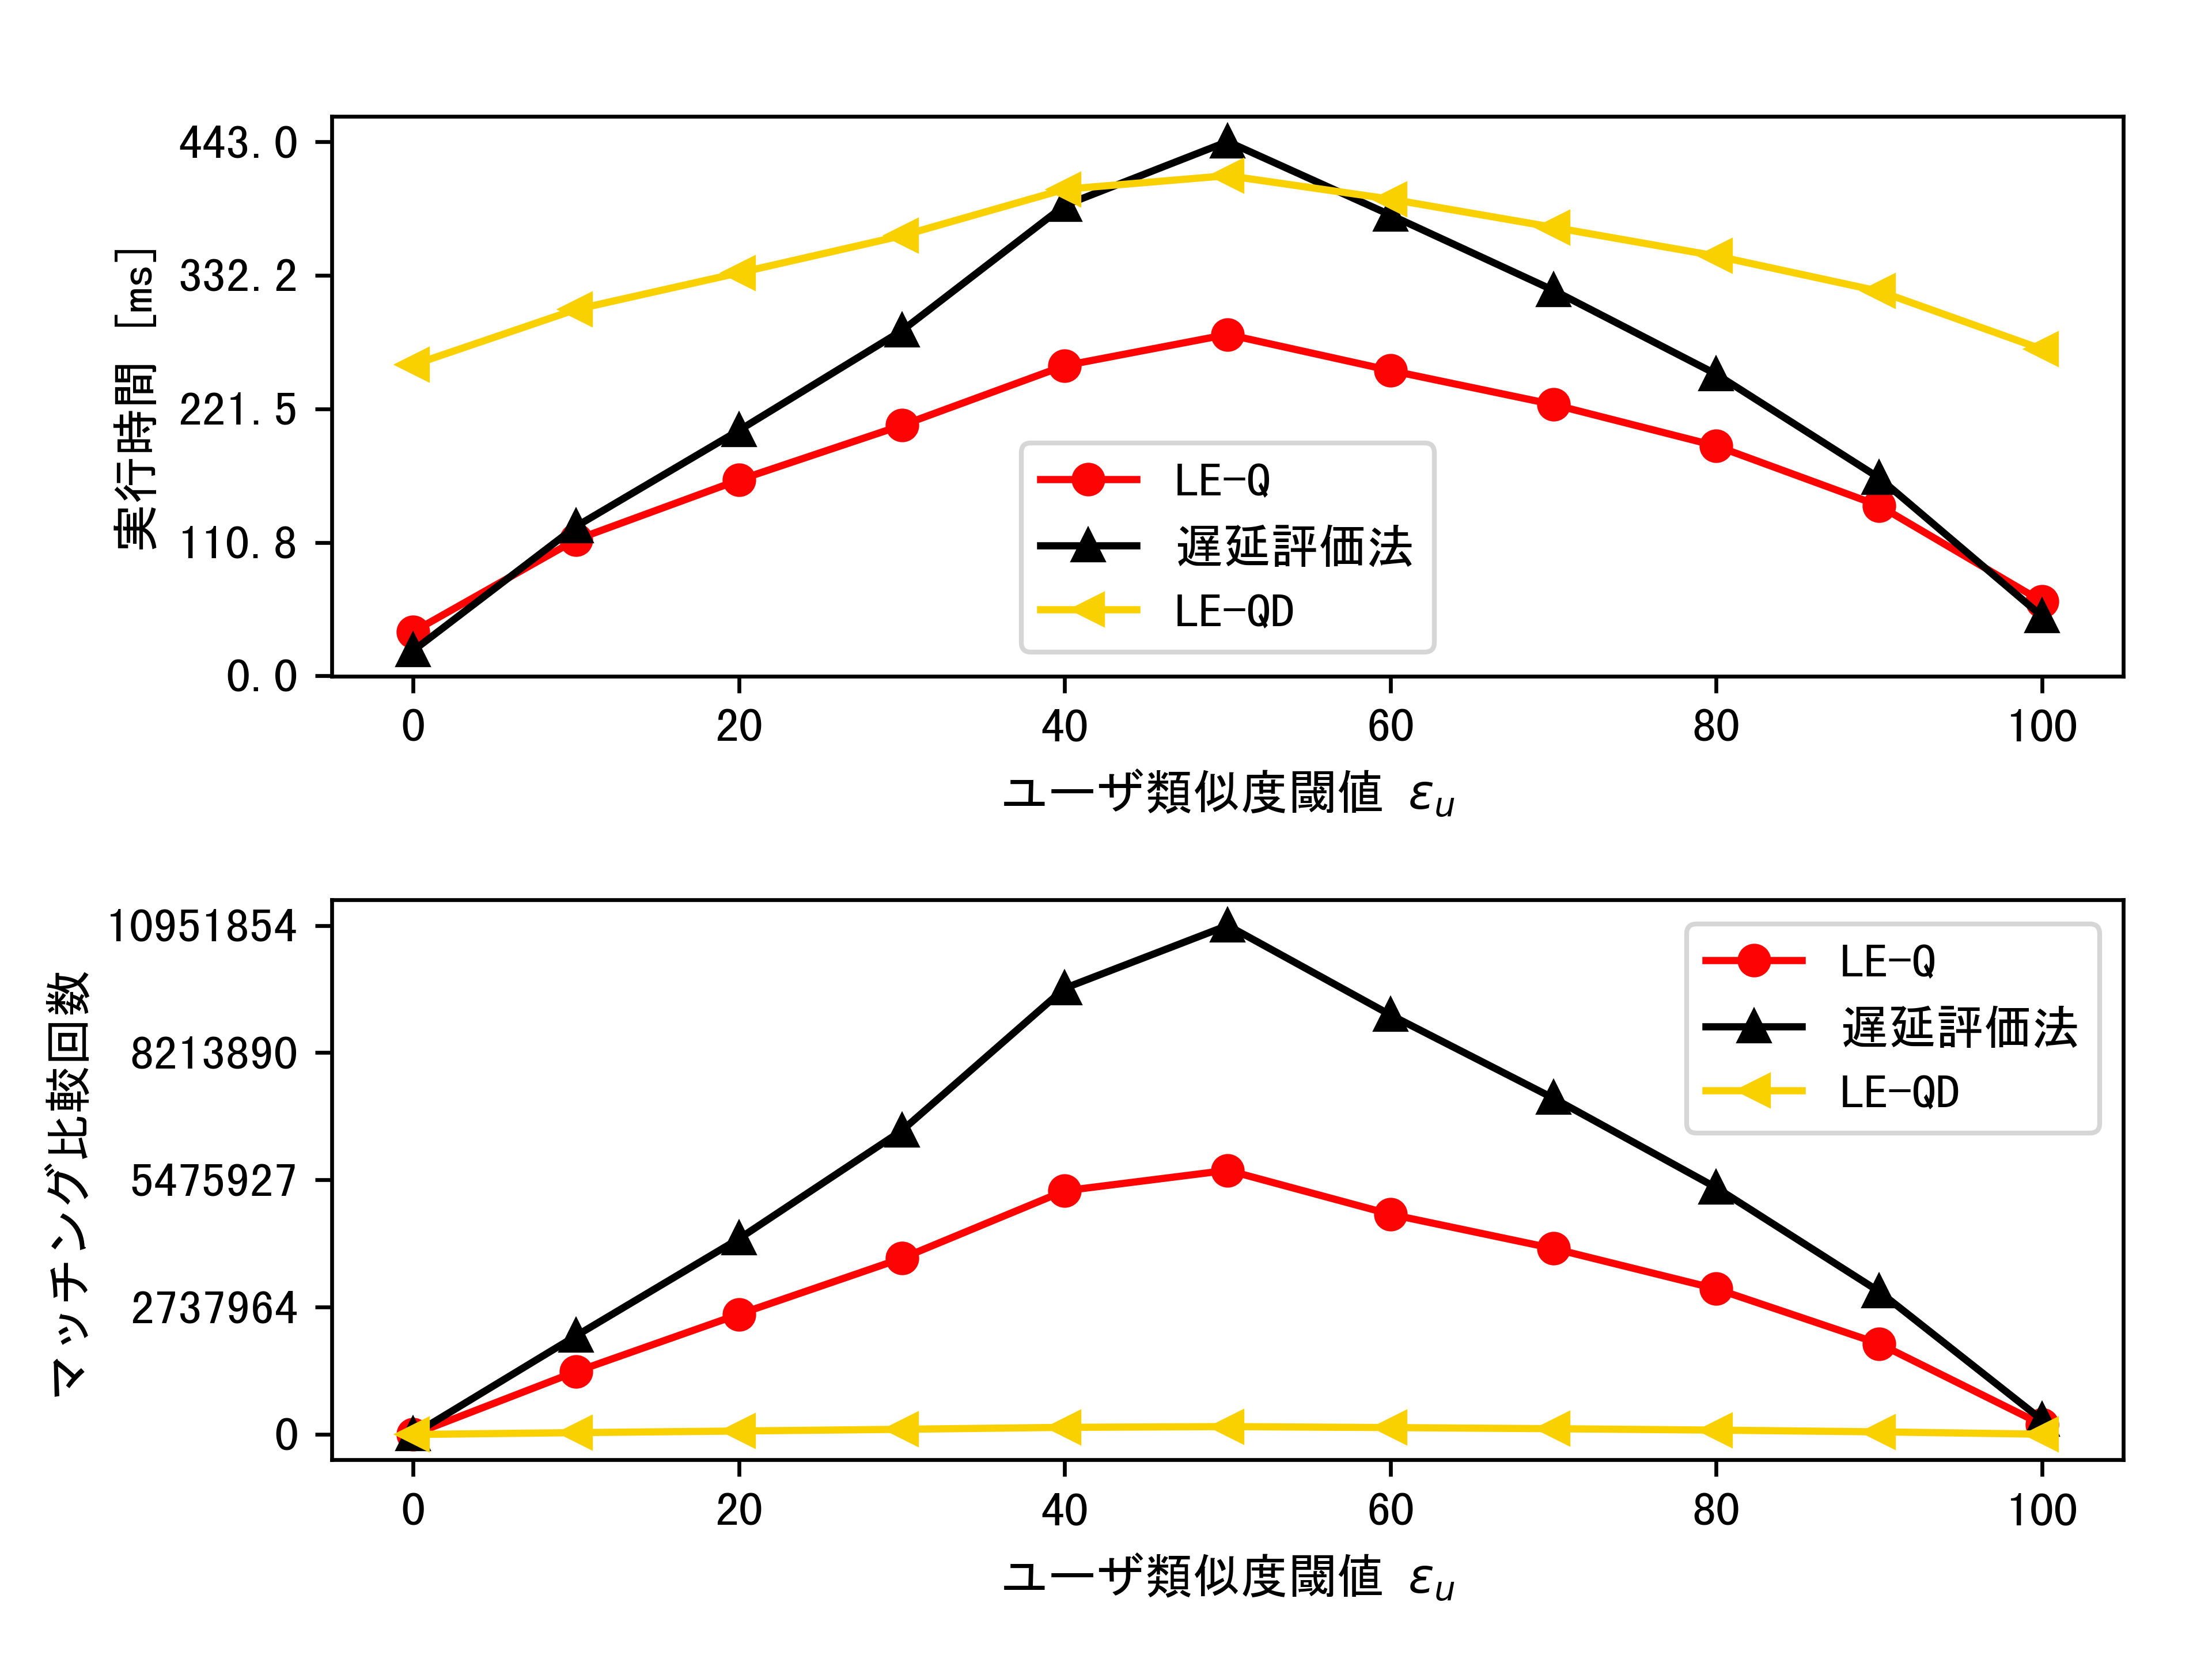
\includegraphics[width=8.3cm]{eimg/exp1_7.png}
    \caption{性能評価(人工データセット($p=0.7$))}
    \label{fig:exp1_art_7}
\end{figure}
\begin{figure}[H]
    \centering
    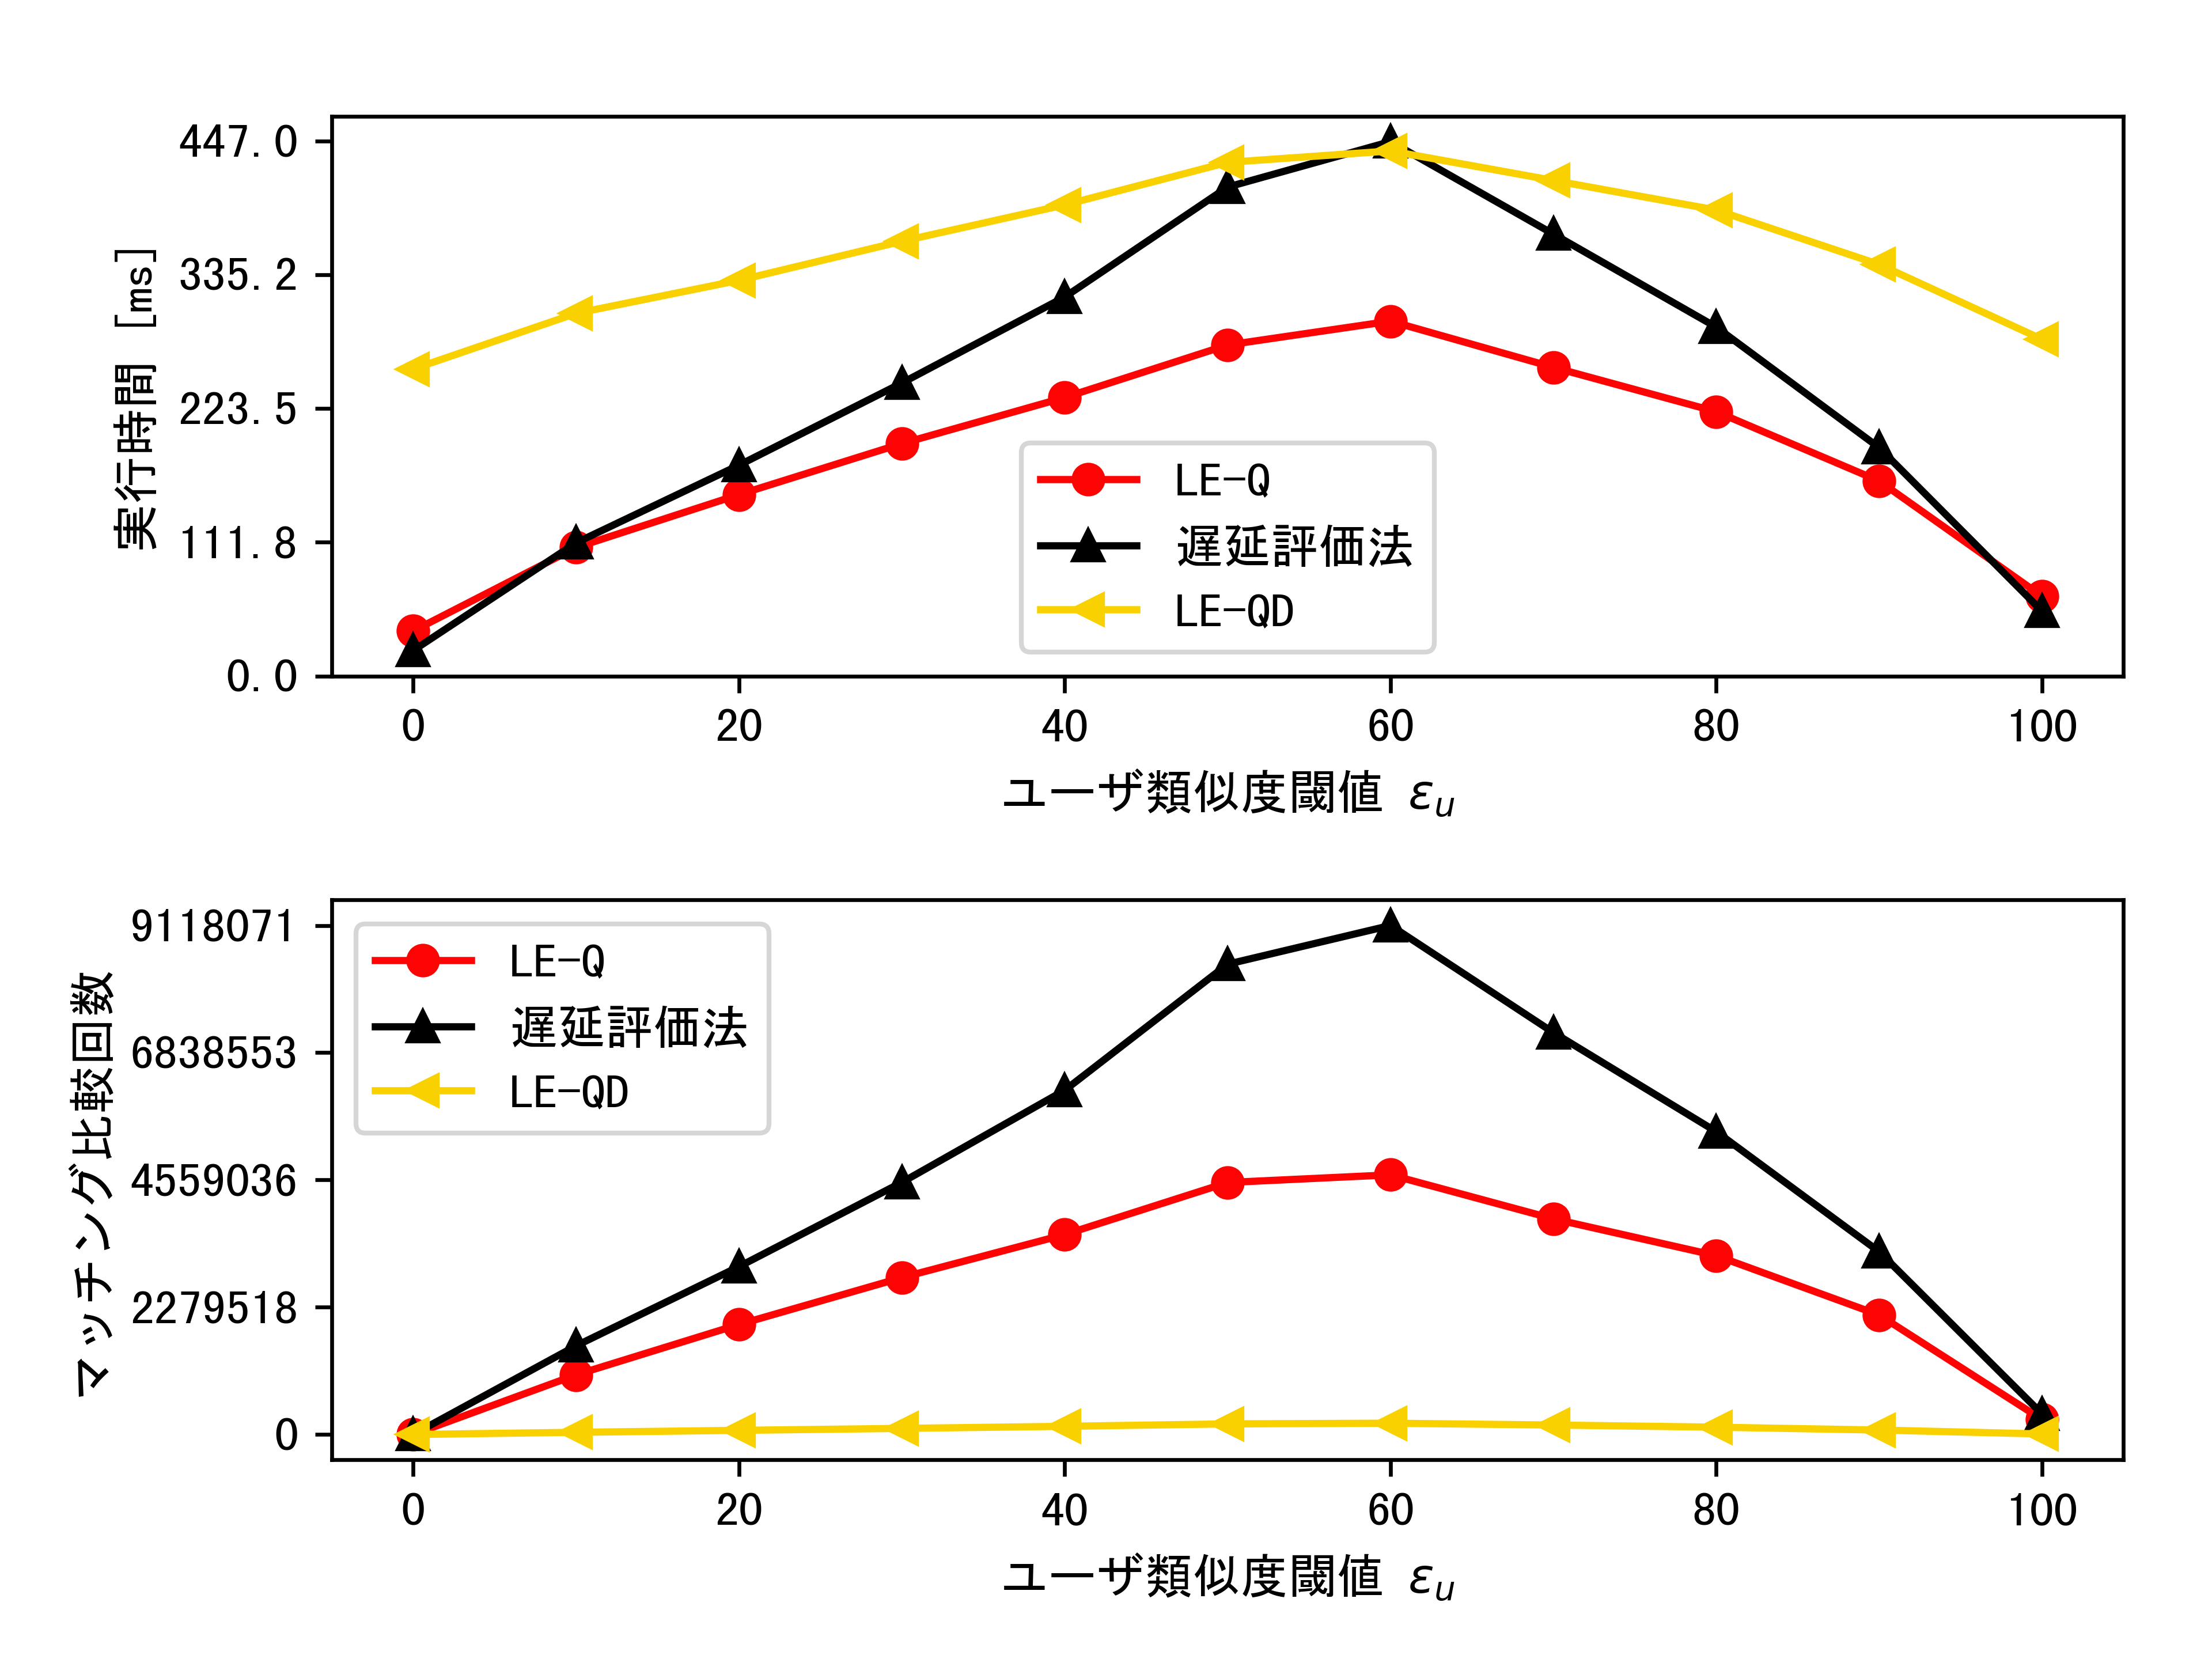
\includegraphics[width=8.3cm]{eimg/exp1_9.png}
    \caption{性能評価(人工データセット($p=0.9$))}
    \label{fig:exp1_art_9}
\end{figure}



\section{マッチング順序の評価}
\ref{exp1}節の実験からLE-QDよりもLE-Qの方が優れていると考えられるため,本実験ではLE-Qを対象とする.
\ref{order_matching}節で示したとおりマッチング順序に関しては新しいテキストから優先してマッチング判定をすることが効率的であると考えられるが,この優位性が転置インデクスを用いたアルゴリズムでも確認できるかを調べる.そのためにLE-Qにおけるマッチング処理を古いテキスト優先のマッチング処理に置き換え,全ユーザの類似性を各時刻すべてにおいて求める実験を行った.
人工データセットにおける実験結果を図\ref{fig:exp2}に示した.
結果より,新しいテキストから優先的にマッチングする方が実行時間が短縮され効果的であることが示された.これは新しいテキスト優先にすることでマッチング比較回数を削減することが出来た影響であると考える.

\begin{figure}[H]
    \centering
    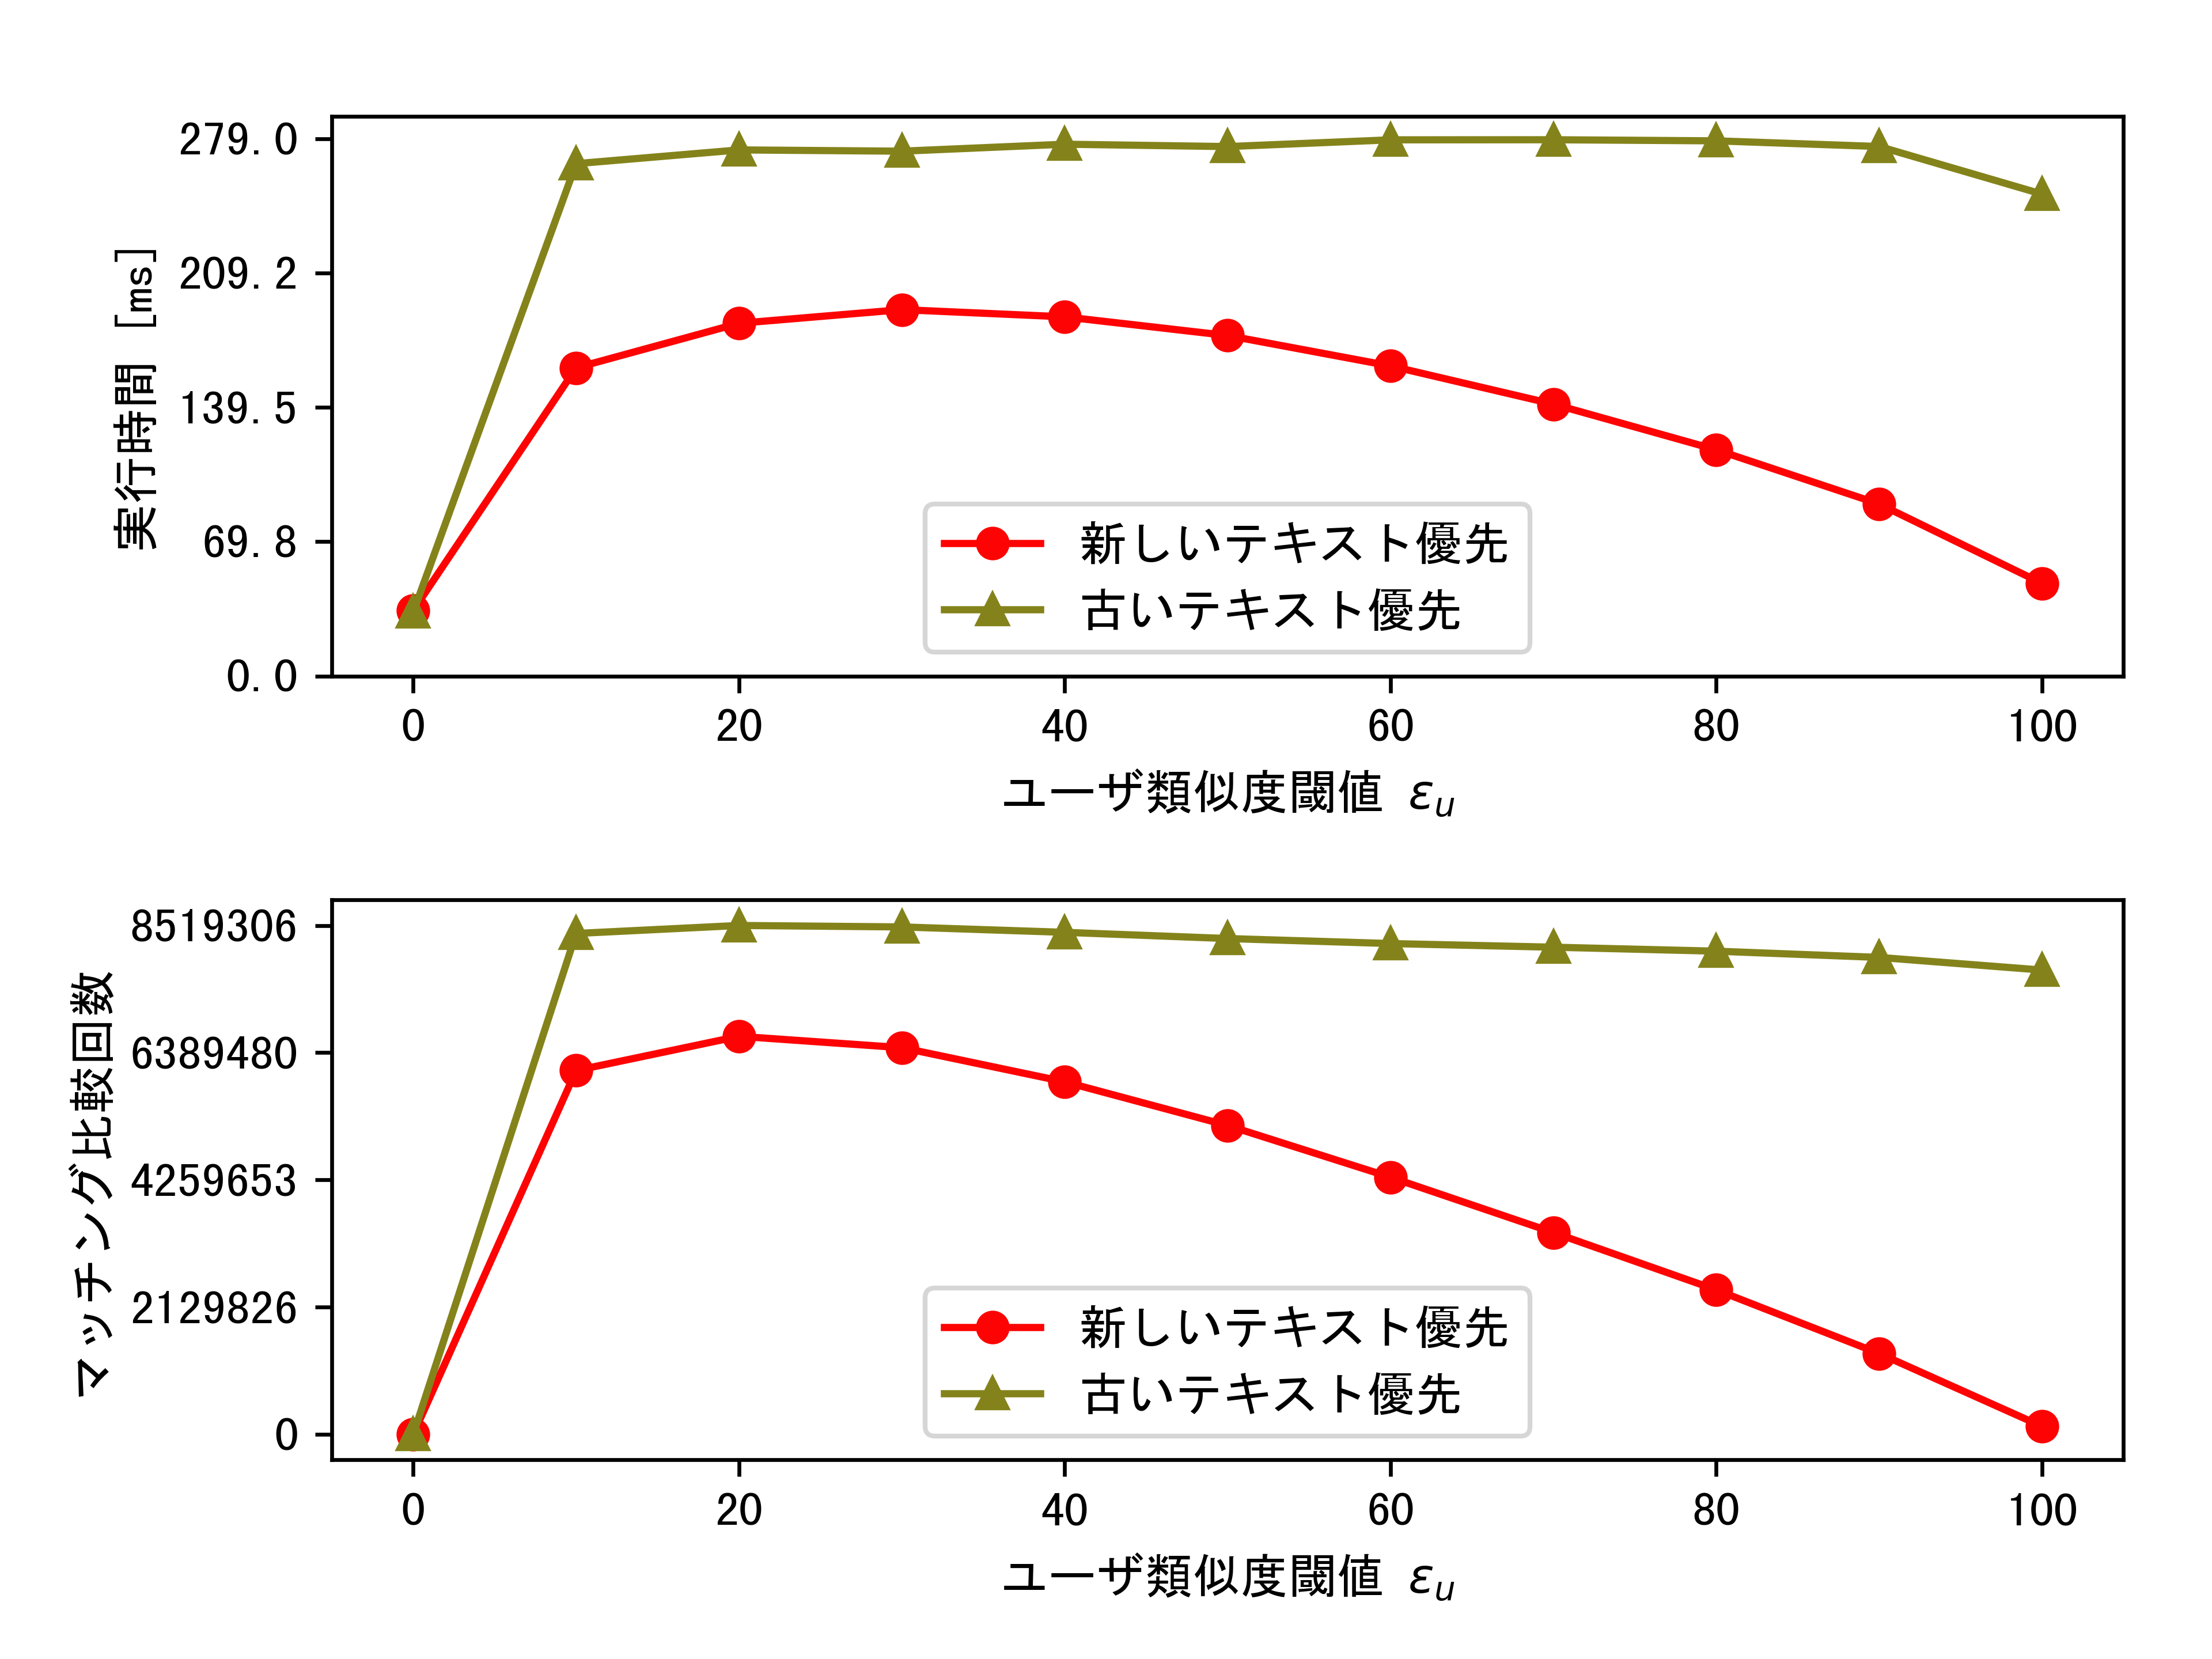
\includegraphics[width=8.3cm]{eimg/exp2.png}
    \caption{LE-Qのマッチング順序の優位性評価(人工データセット($p=0.96^{(i-1)}$))}
    \label{fig:exp2}
\end{figure}
CoPhIRデータセットにおける実験結果を図\ref{fig:exp2_c}に示した.
図\ref{fig:exp2_c}は人工データによる実験と同様の結果を示し,テキストのマッチング順序として新しいテキストから優先することは有効であると確認できた.
\begin{figure}[H]
    \centering
    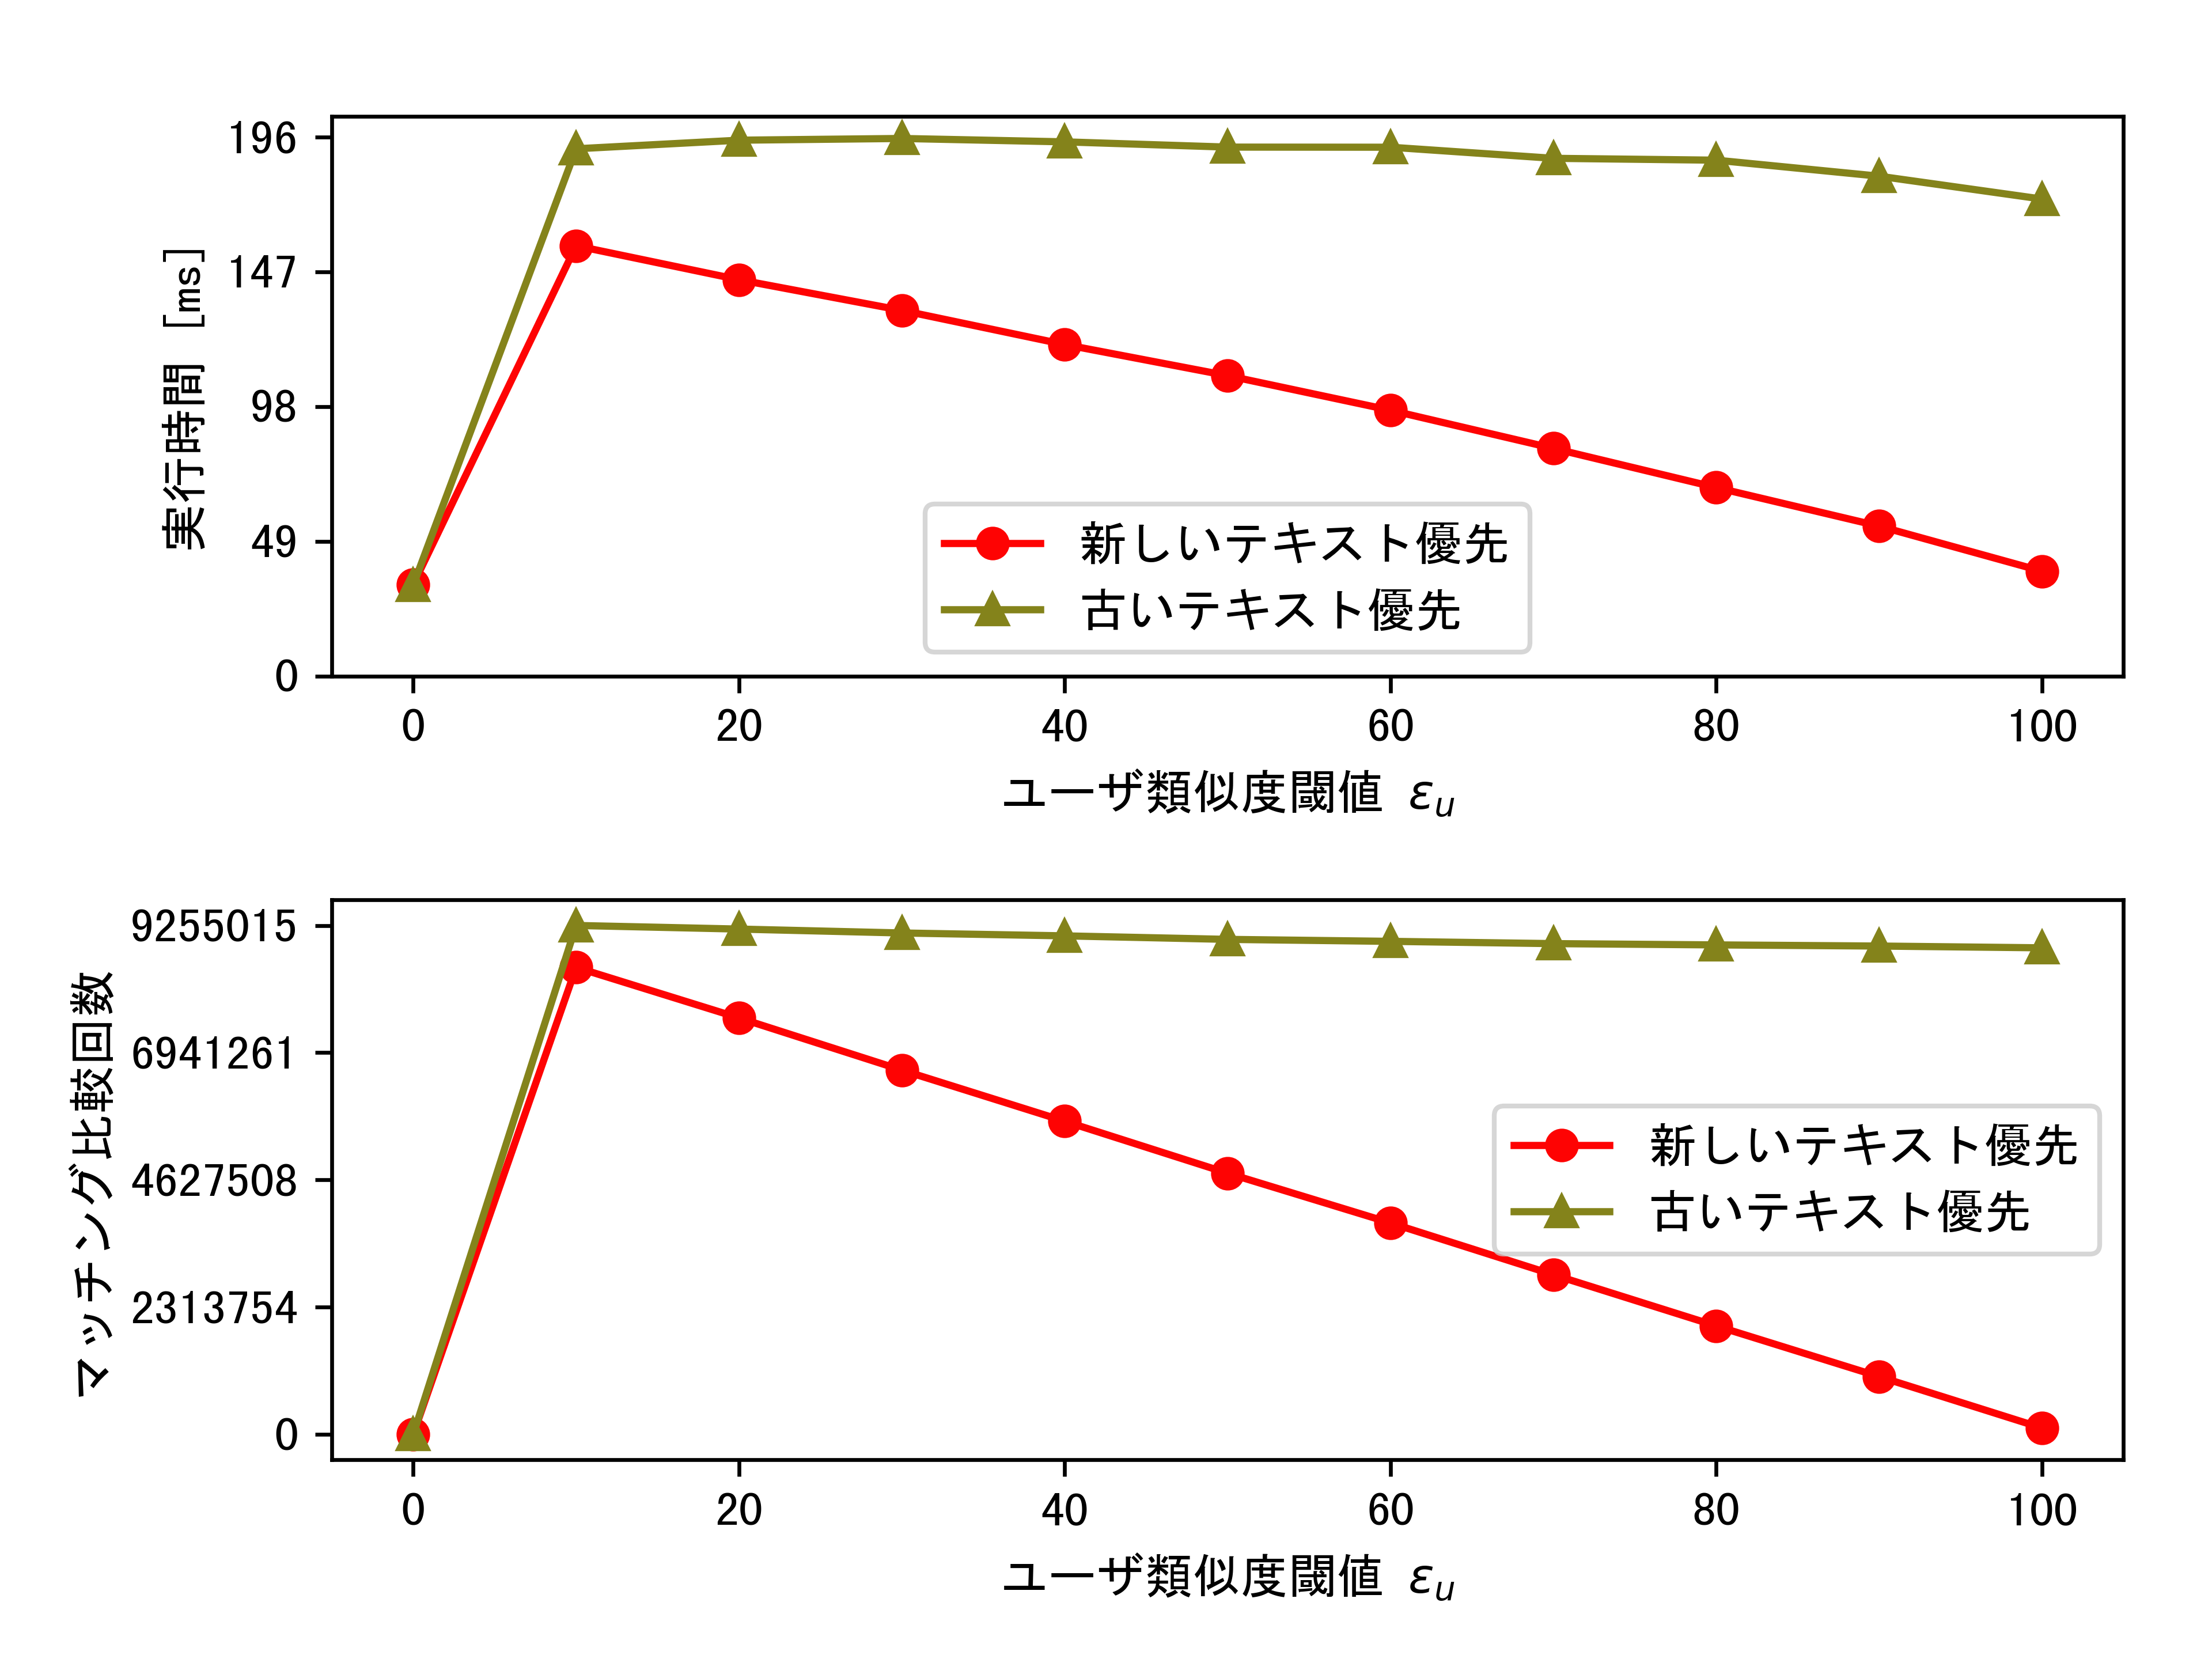
\includegraphics[width=8.3cm]{eimg/exp2_c.png}
    \caption{LE-Qのマッチング順序の優位性評価(CoPhIRデータセット)}
    \label{fig:exp2_c}
\end{figure}

人工データセットにおける$p$を固定した場合の実験結果を図\ref{fig:exp2_1},図\ref{fig:exp2_3},図\ref{fig:exp2_5},図\ref{fig:exp2_7},図\ref{fig:exp2_9}に示した.
$p$の値によらずマッチングには新しいテキストを優先することが効果的であることが示された.

\begin{figure}[H]
    \centering
    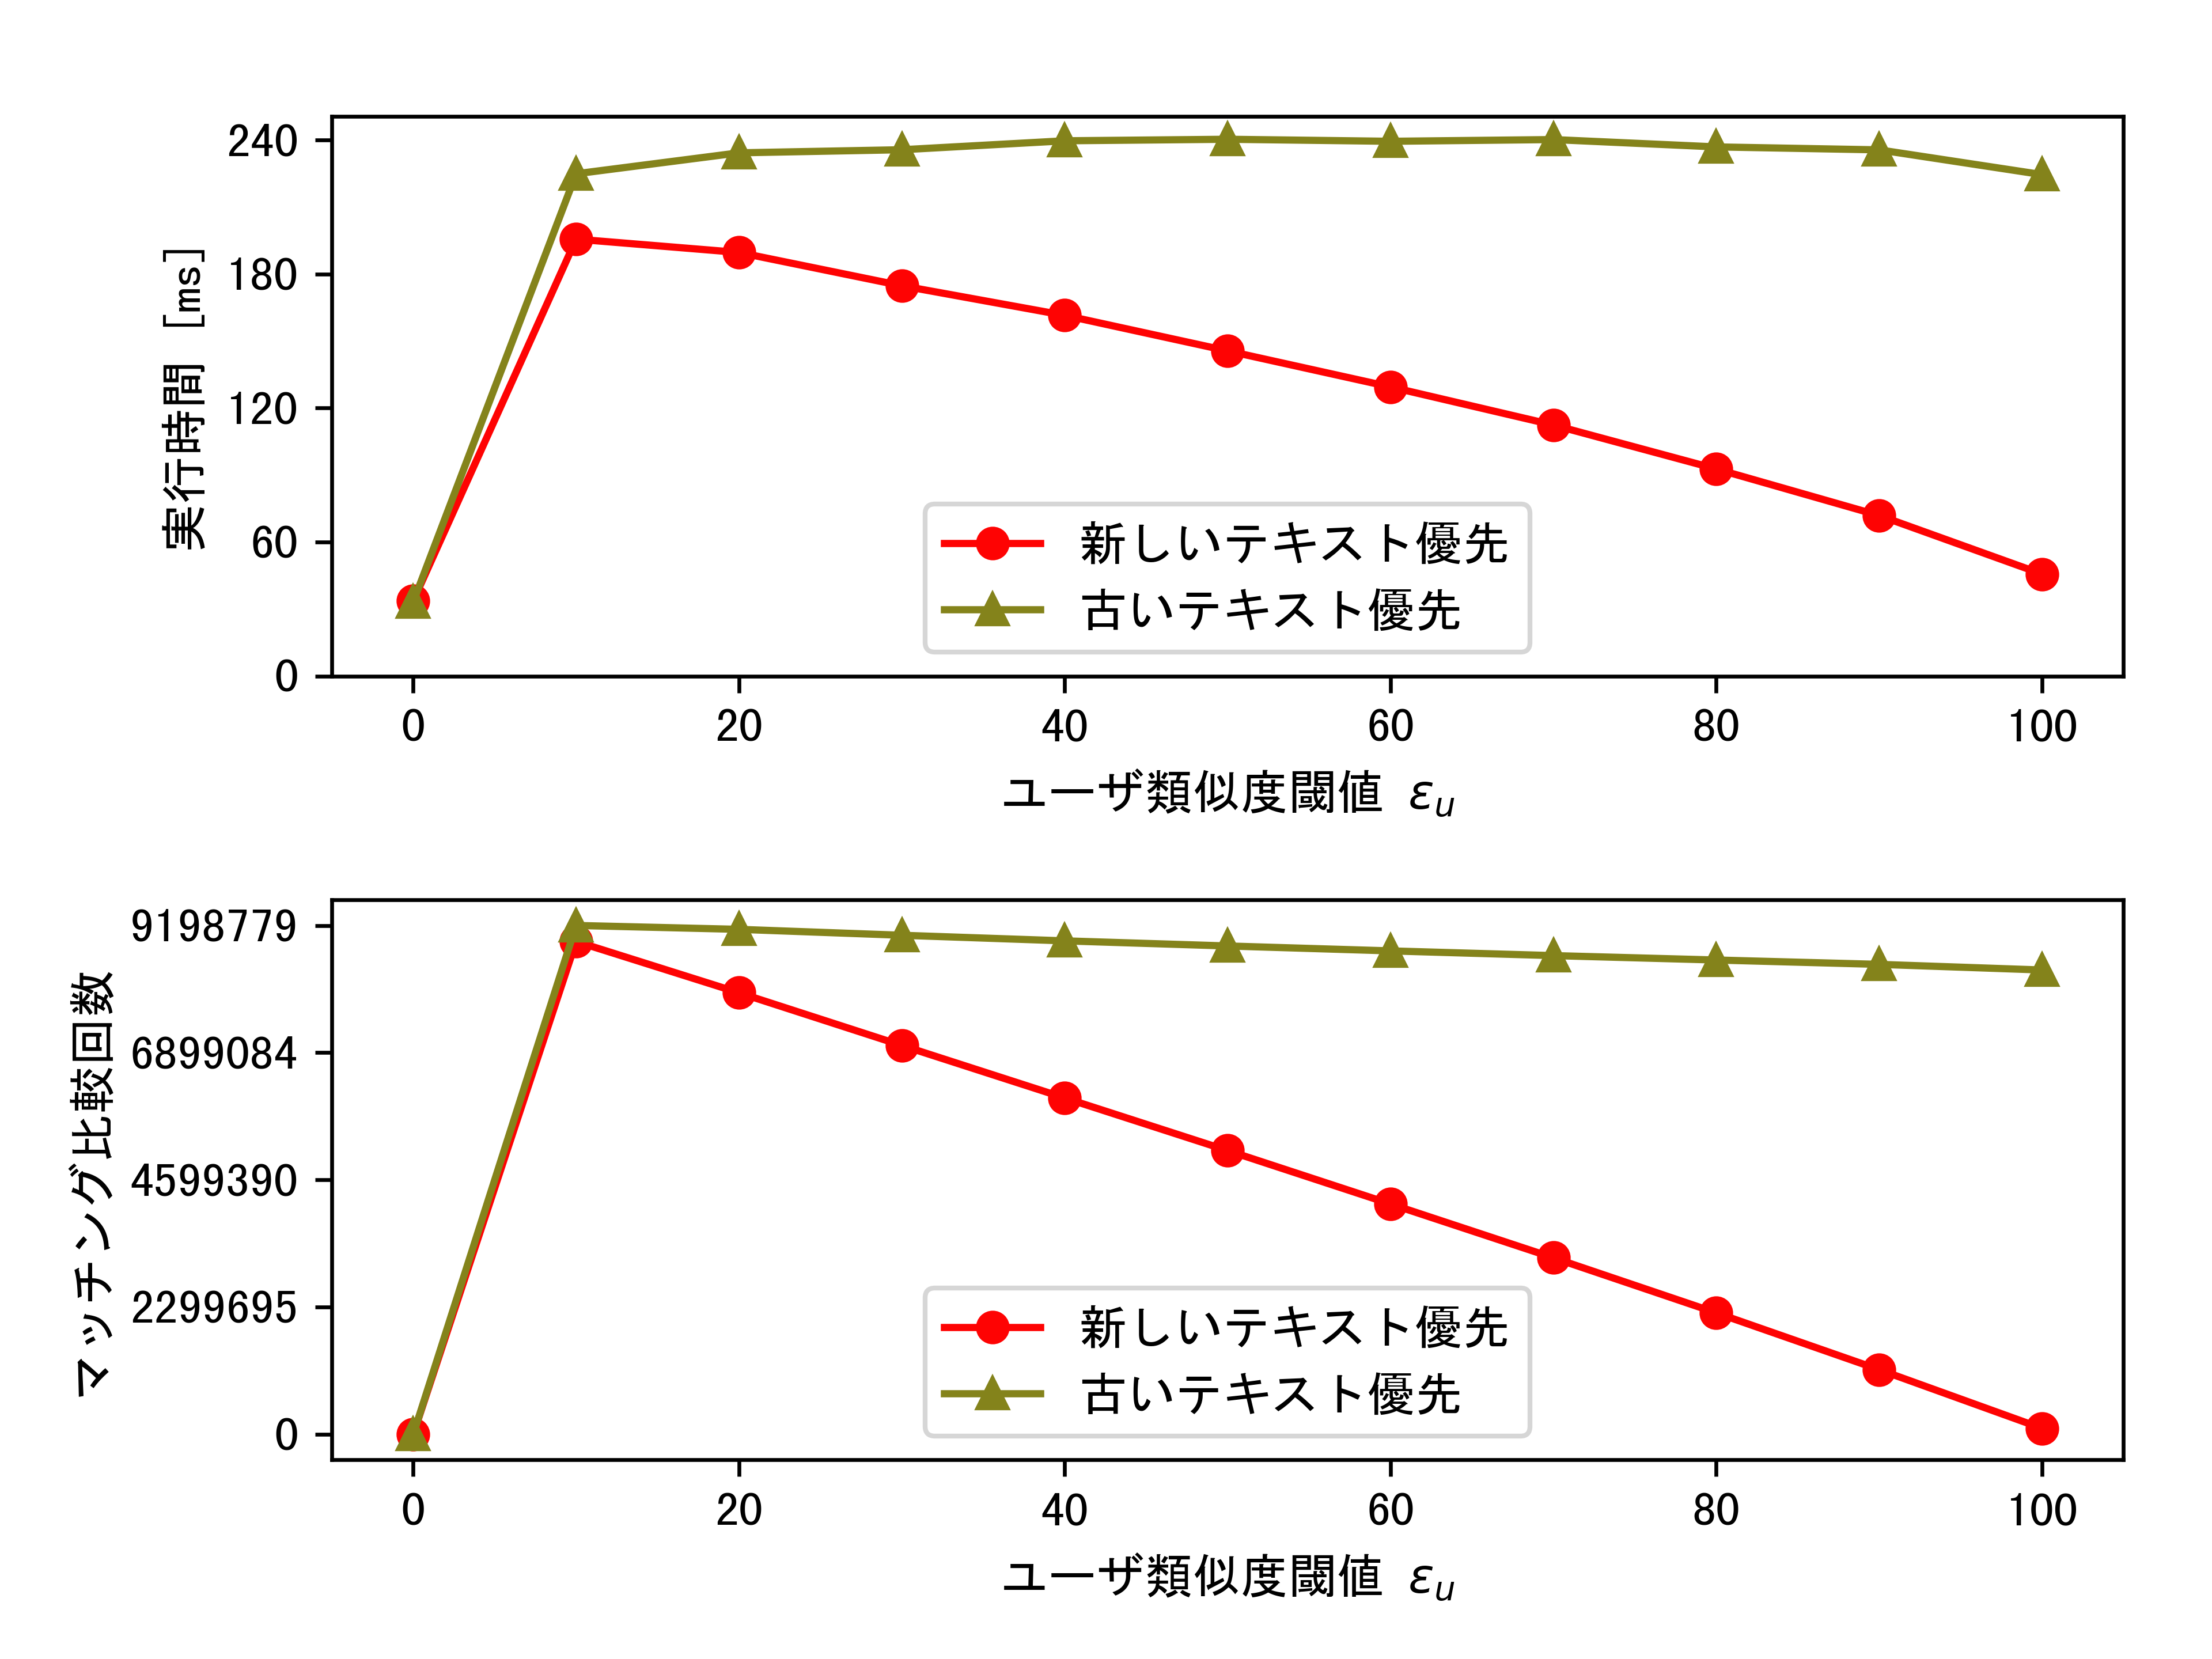
\includegraphics[width=8.3cm]{eimg/exp2_1.png}
    \caption{LE-Qのマッチング順序の優位性評価(人工データセット($p=0.1$))}
    \label{fig:exp2_1}
\end{figure}
\begin{figure}[H]
    \centering
    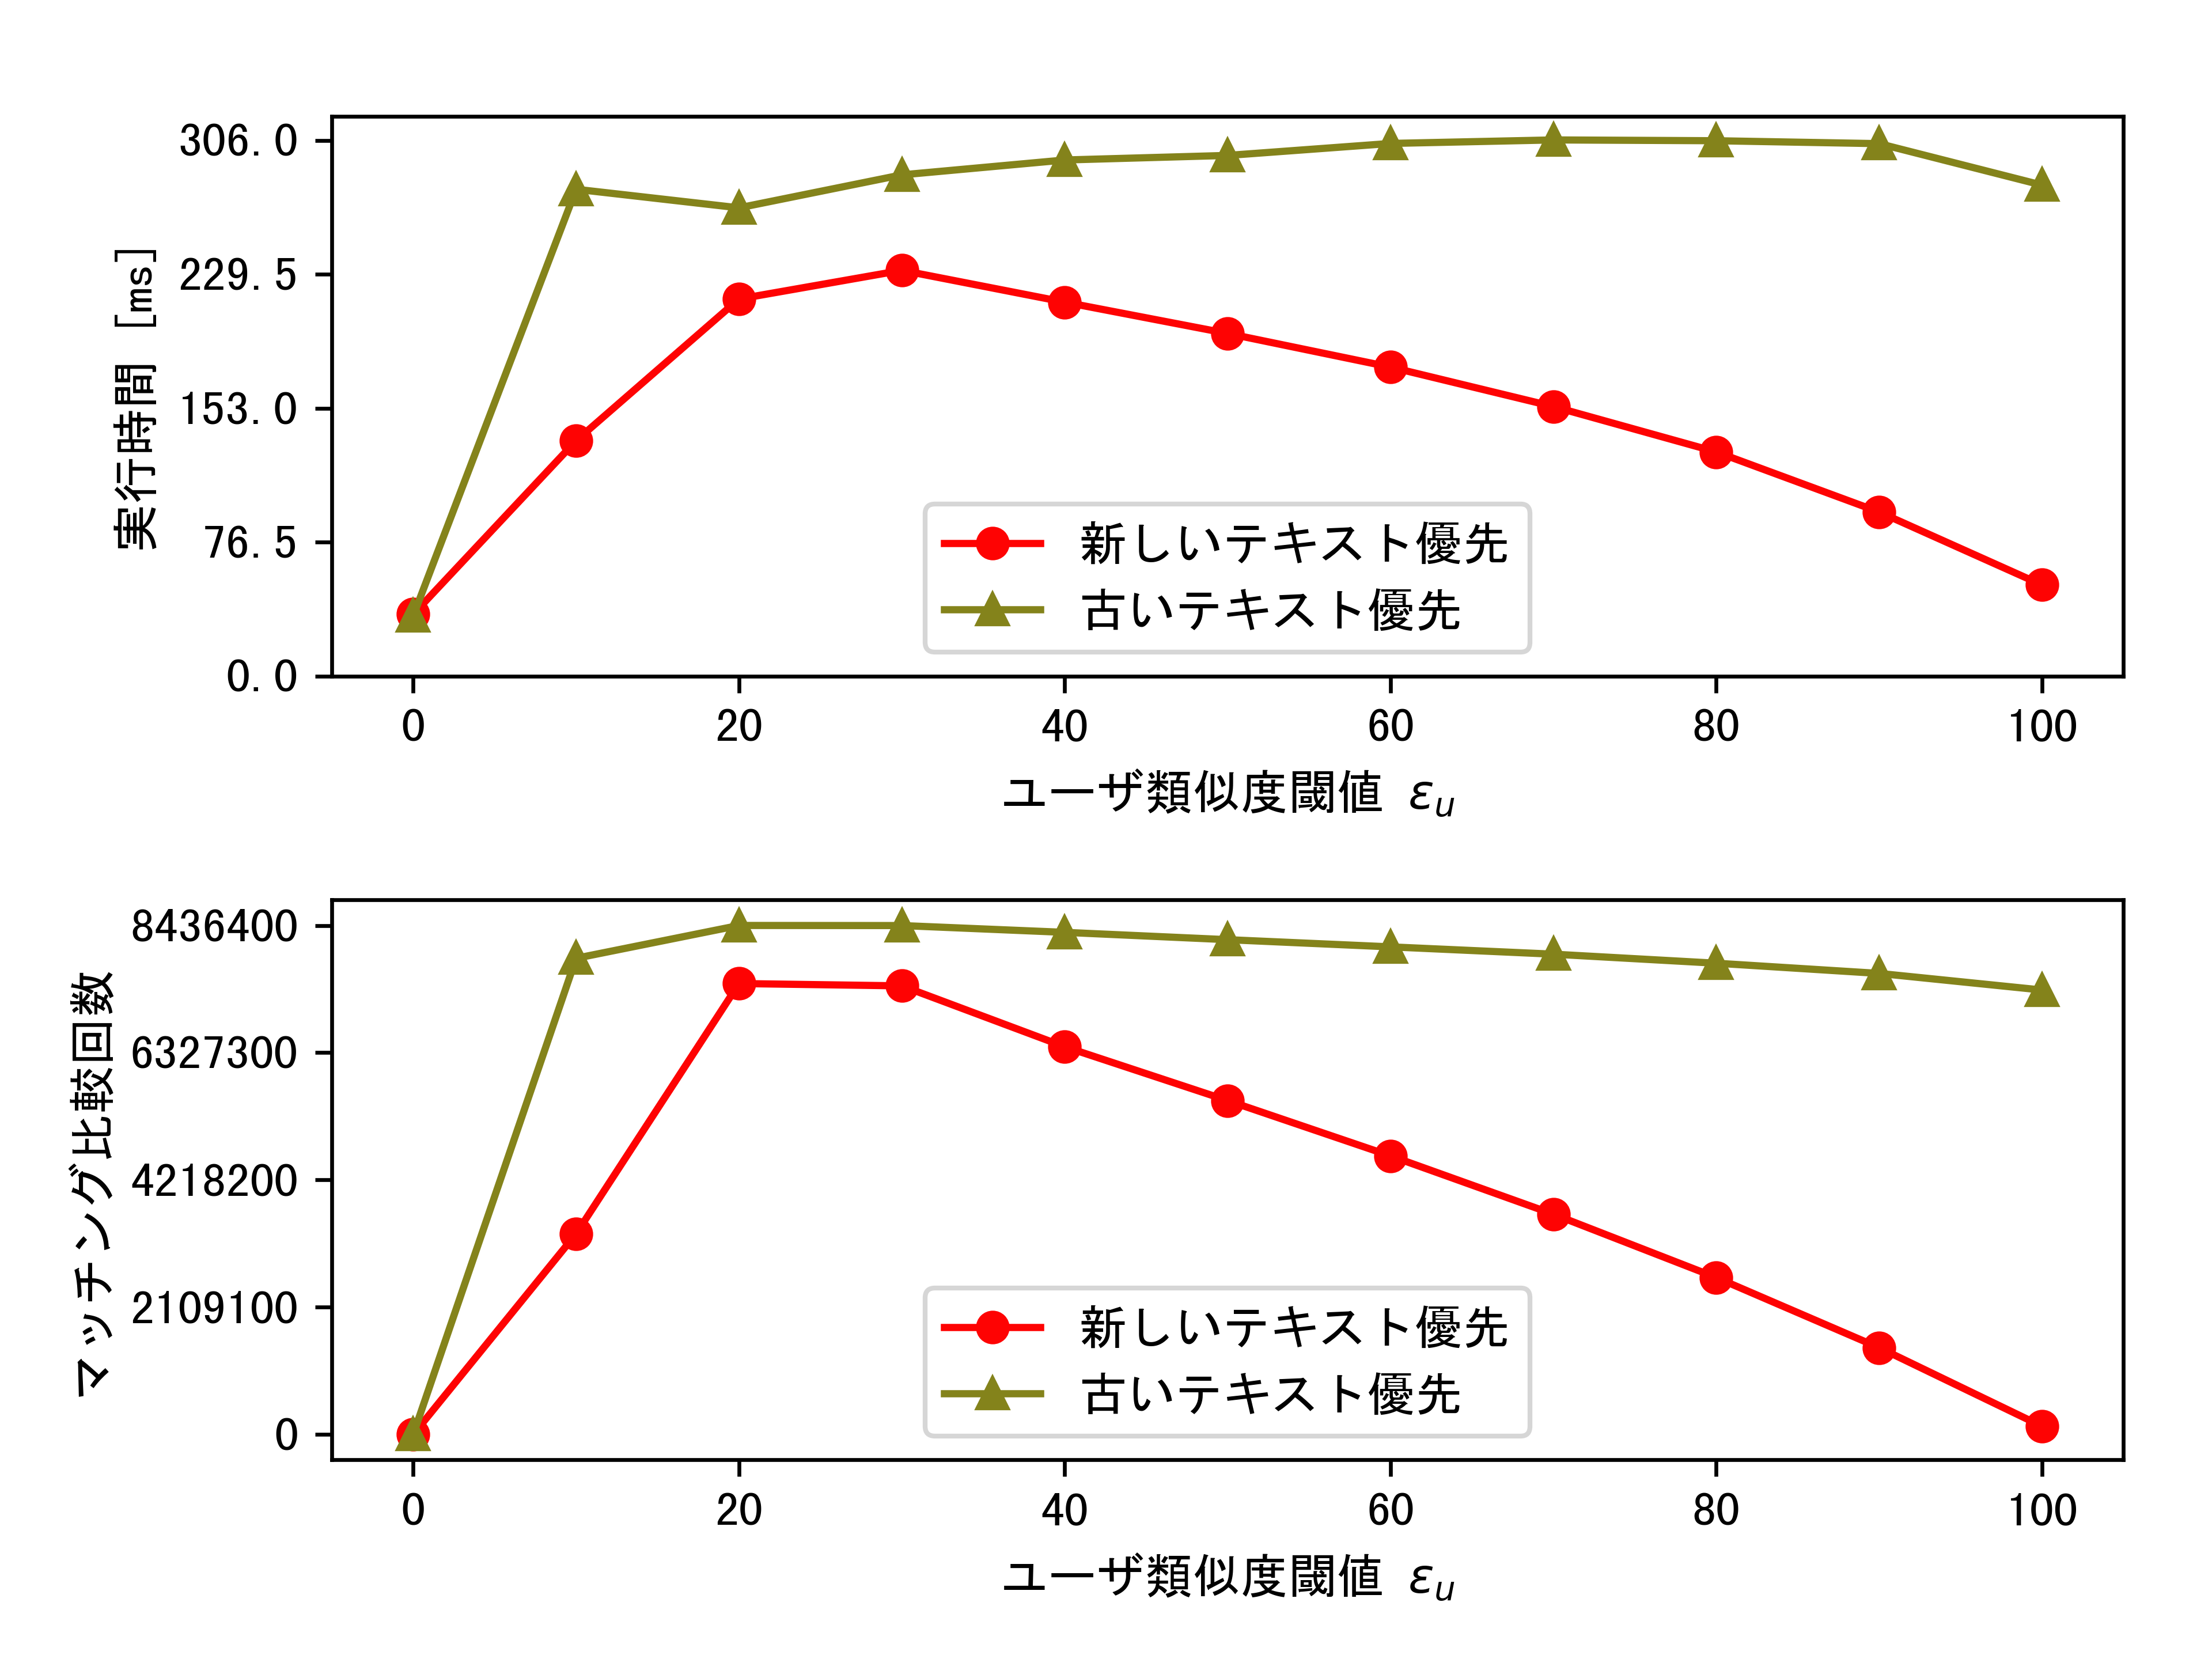
\includegraphics[width=8.3cm]{eimg/exp2_3.png}
    \caption{LE-Qのマッチング順序の優位性評価(人工データセット($p=0.3$))}
    \label{fig:exp2_3}
\end{figure}
\begin{figure}[H]
    \centering
    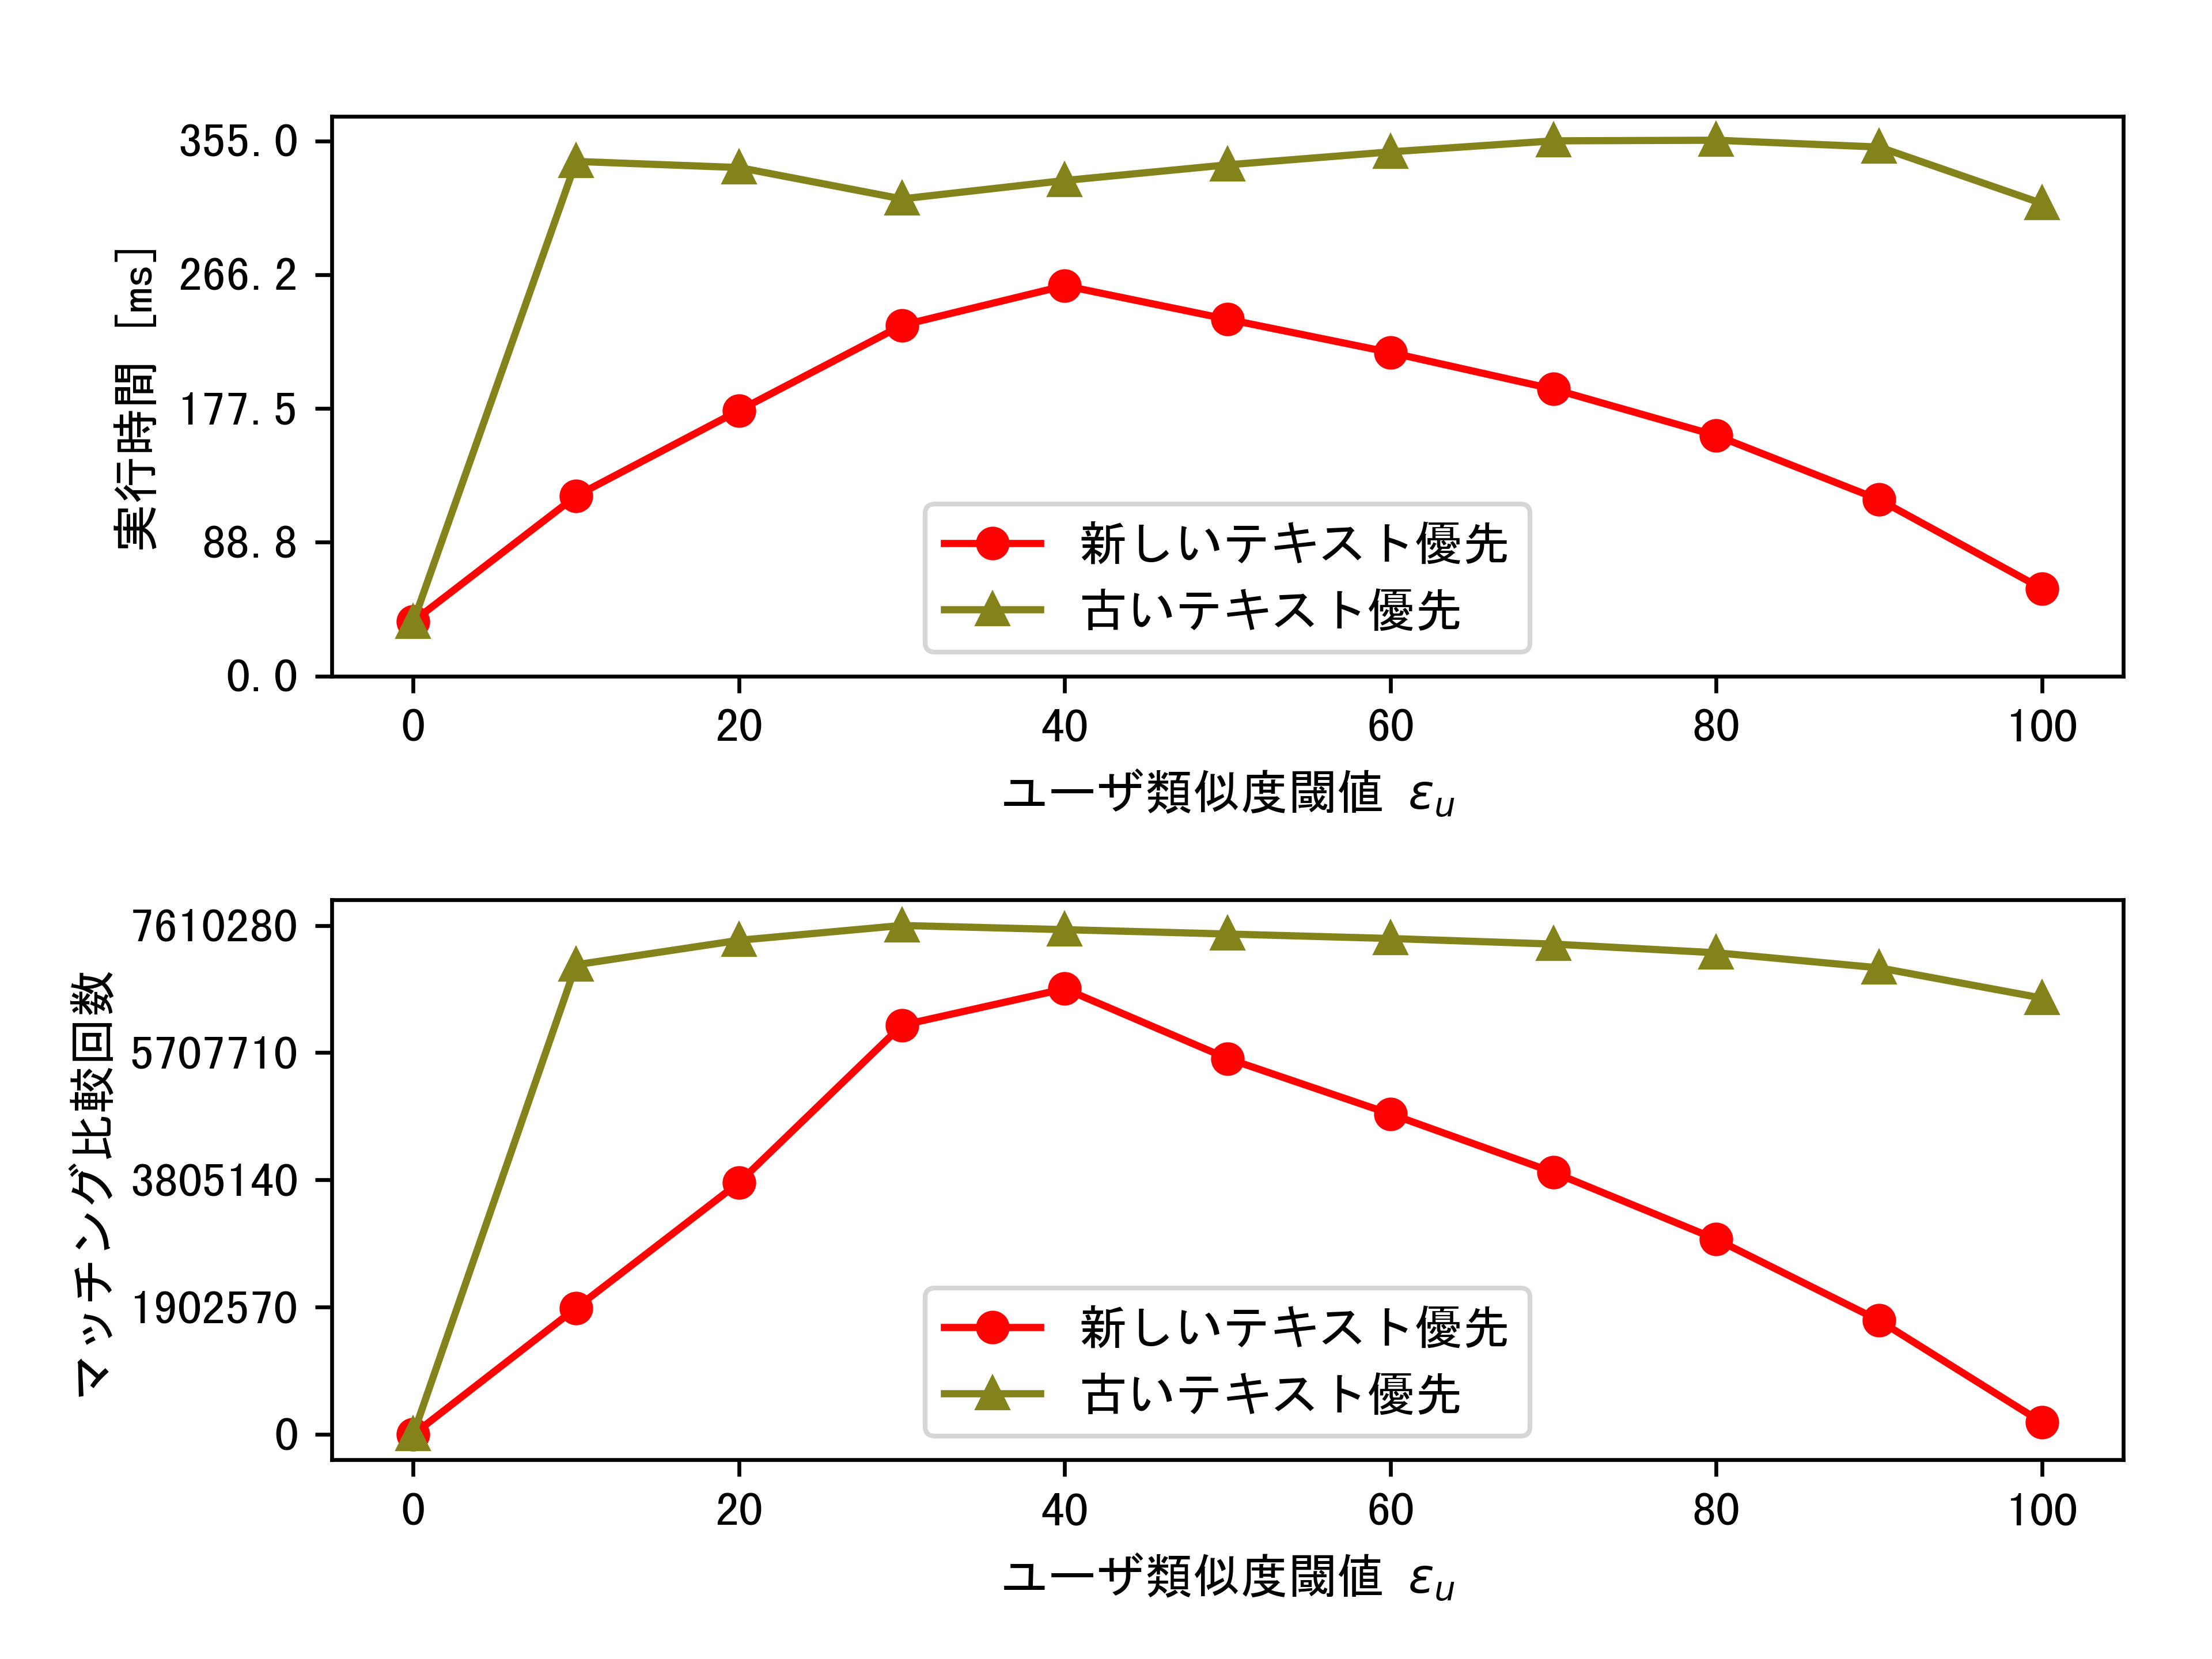
\includegraphics[width=8.3cm]{eimg/exp2_5.png}
    \caption{LE-Qのマッチング順序の優位性評価(人工データセット($p=0.5$))}
    \label{fig:exp2_5}
\end{figure}
\begin{figure}[H]
    \centering
    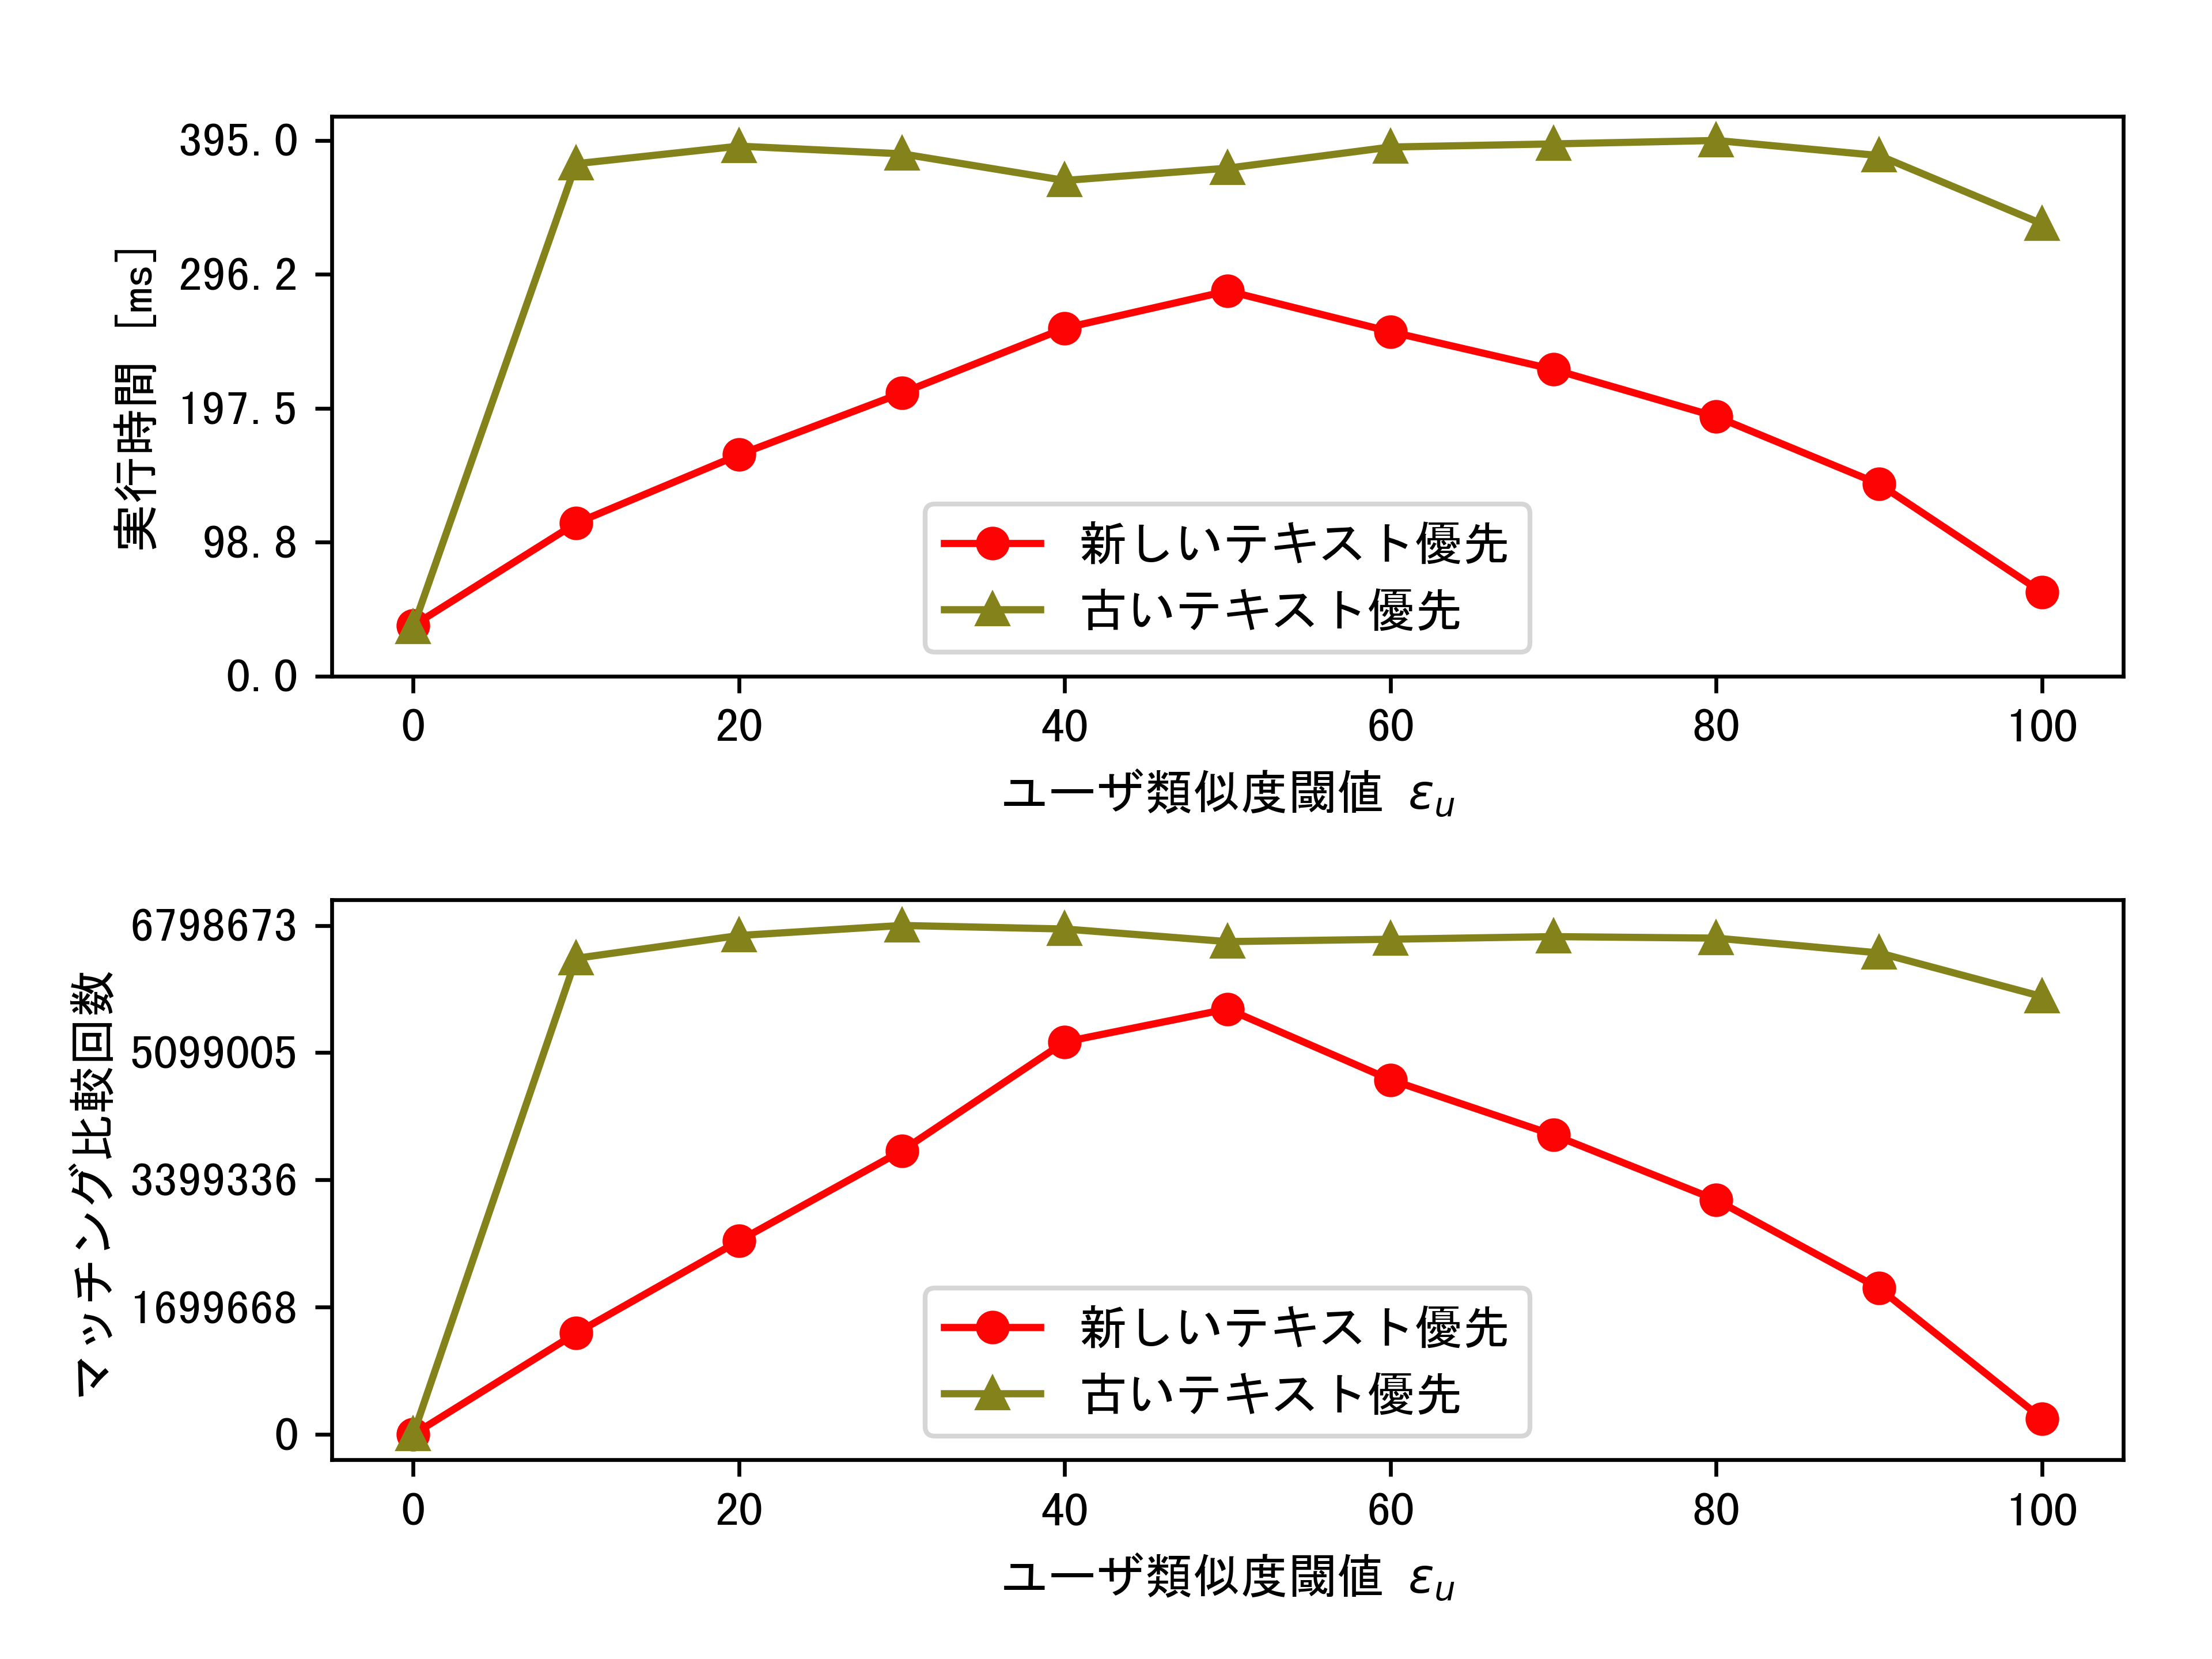
\includegraphics[width=8.3cm]{eimg/exp2_7.png}
    \caption{LE-Qのマッチング順序の優位性評価(人工データセット($p=0.7$))}
    \label{fig:exp2_7}
\end{figure}
\begin{figure}[H]
    \centering
    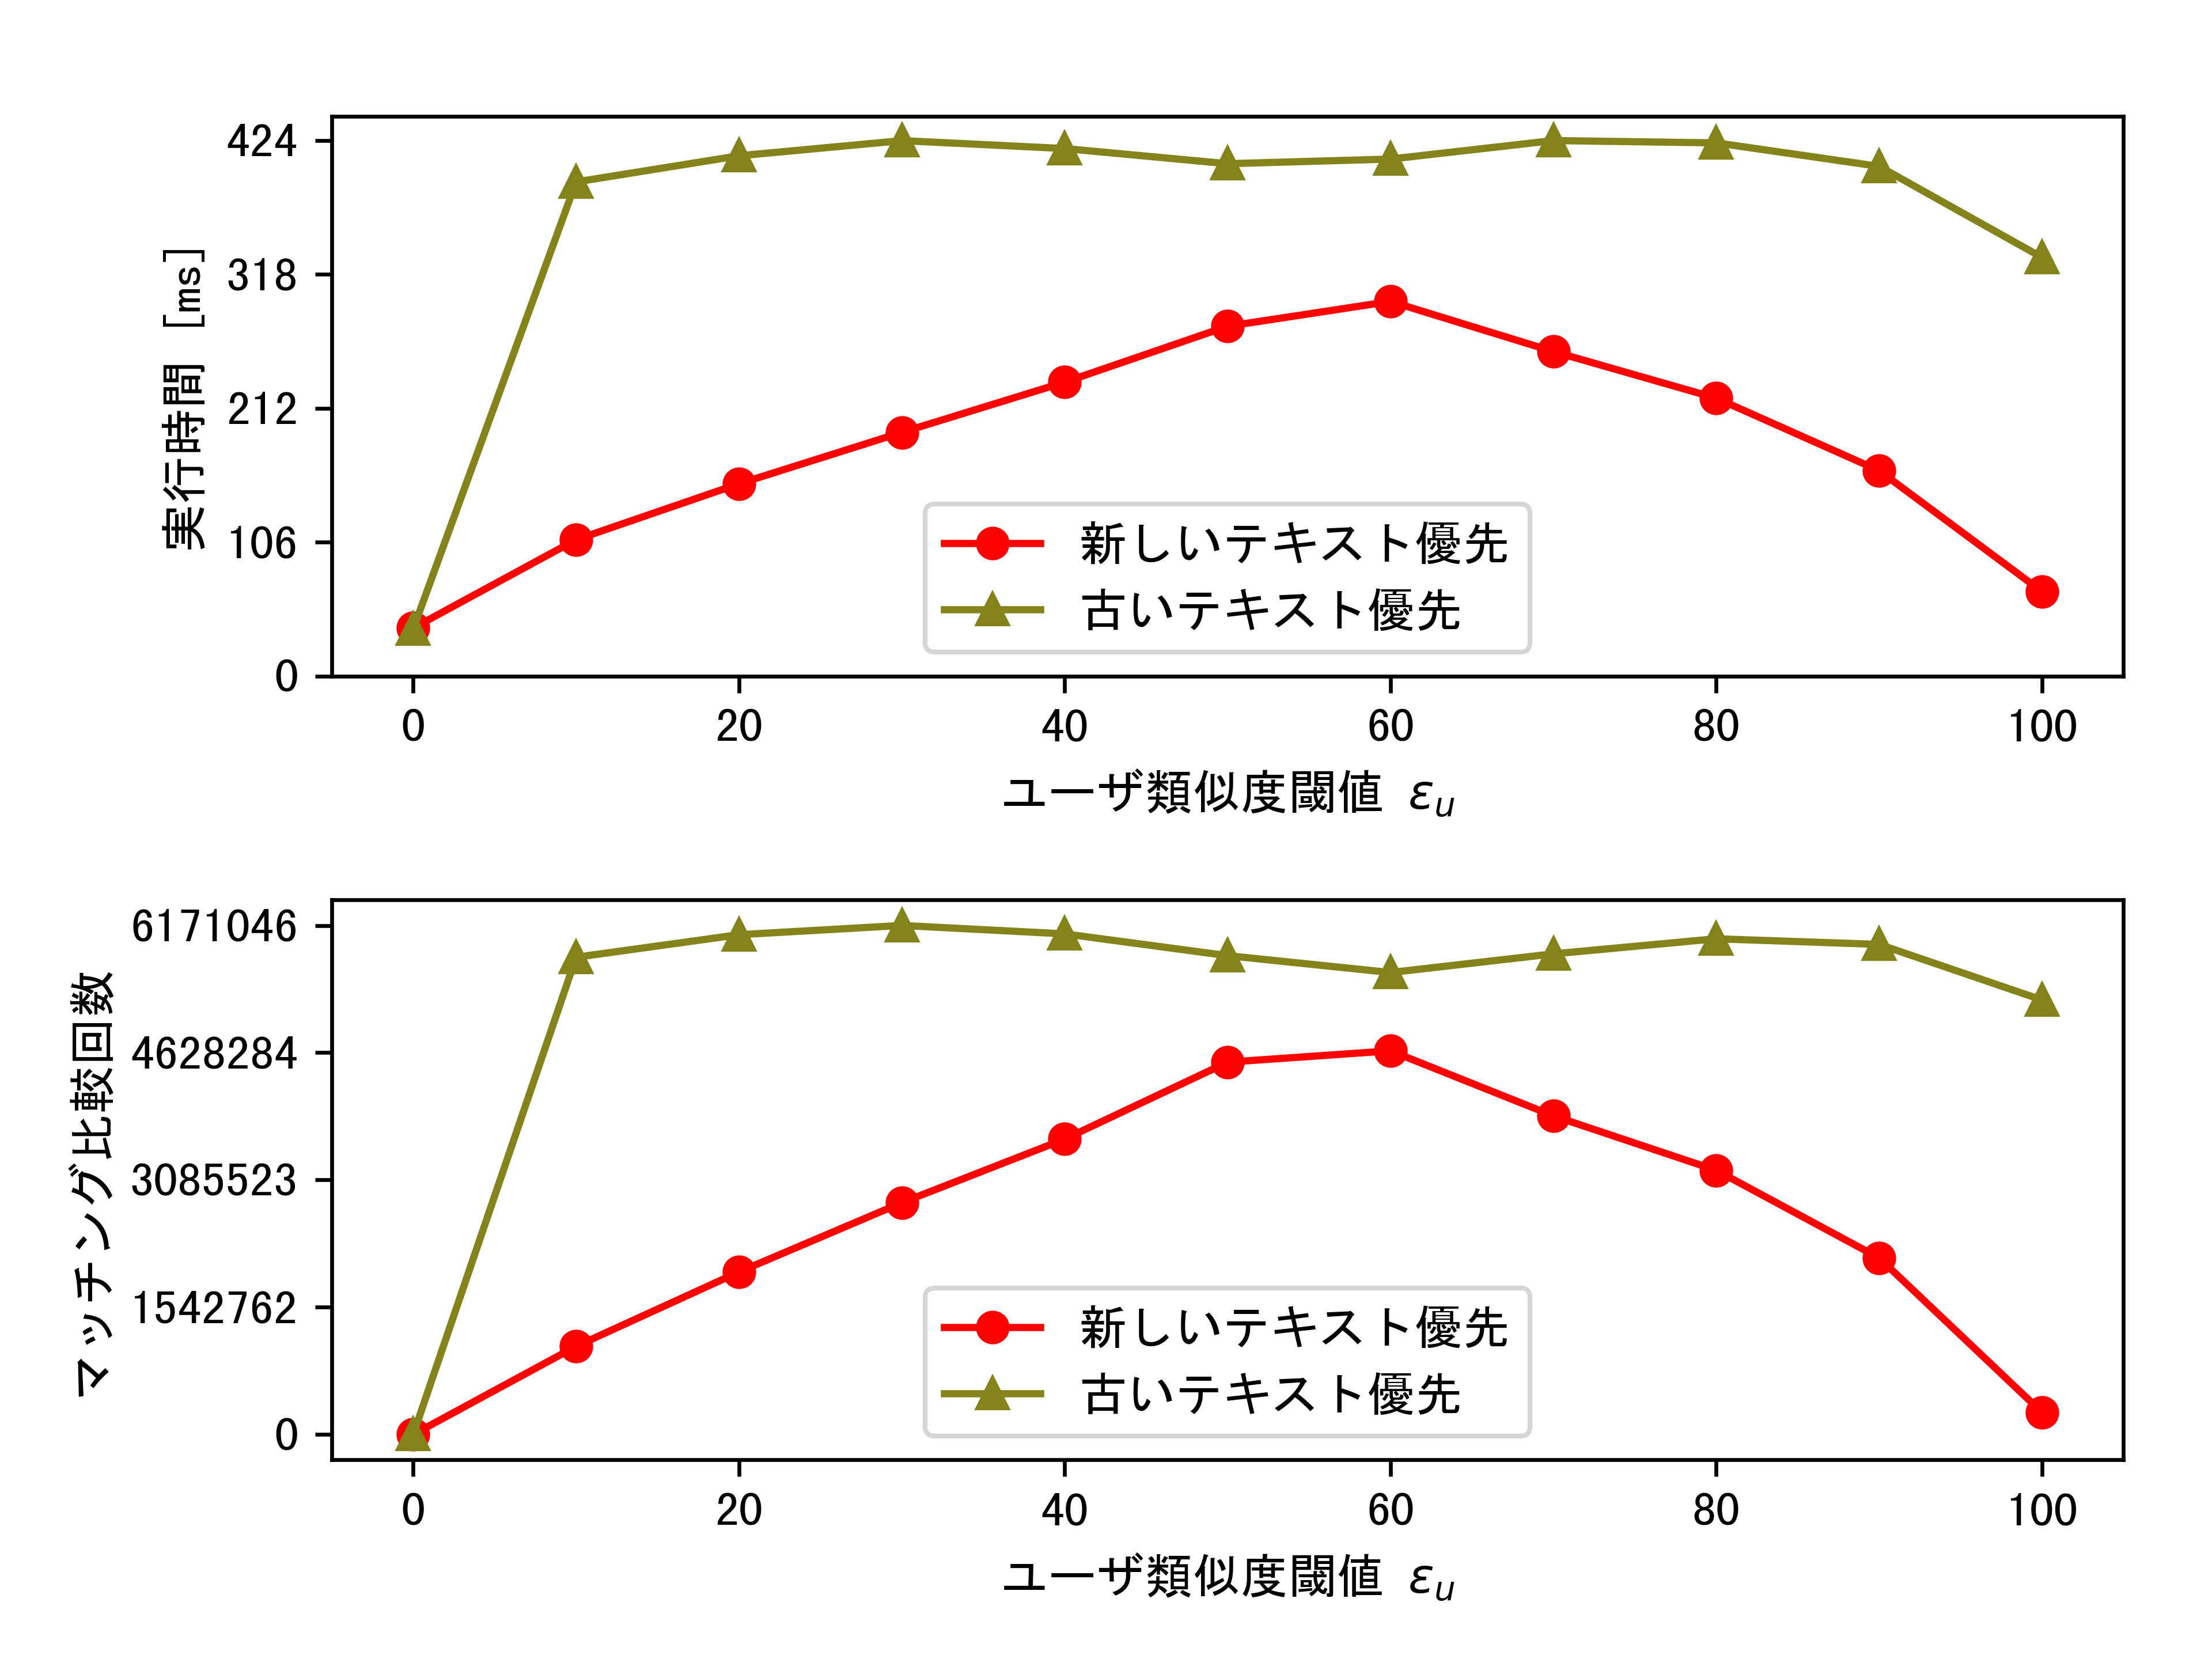
\includegraphics[width=8.3cm]{eimg/exp2_9.png}
    \caption{LE-Qのマッチング順序の優位性評価(人工データセット($p=0.9$))}
    \label{fig:exp2_9}
\end{figure}



\section{ALE-Qの評価}
遅延評価法,LE-Q,LE-Qの改善案であるALE-Qを比較するために,全ユーザの類似性を各時刻すべてにおいて求める実験を行った.$\epsilon_r$を40,$\epsilon_m$を5としたときの人工データセットにおける実験結果を図\ref{fig:exp3}に示した.
結果より,ALE-Qの方がLE-Qより実行時間が短くなっていることがわかる.これはある程度少ない数のテキストのマッチング判定を行わなくてはいけないとき,転置インデクスを用いたマッチングに変更することで共通の単語を1つも持たないテキストへのマッチングを避けることができたからであると考える.さらにかなり少ない数のテキストのマッチング判定を行わなくてはいけないとき,転置インデクスを用いないマッチング方法にすることでマッチング判定を行うテキストの個数を減らすことが出来たからであると考える.

\begin{figure}[H]
    \centering
    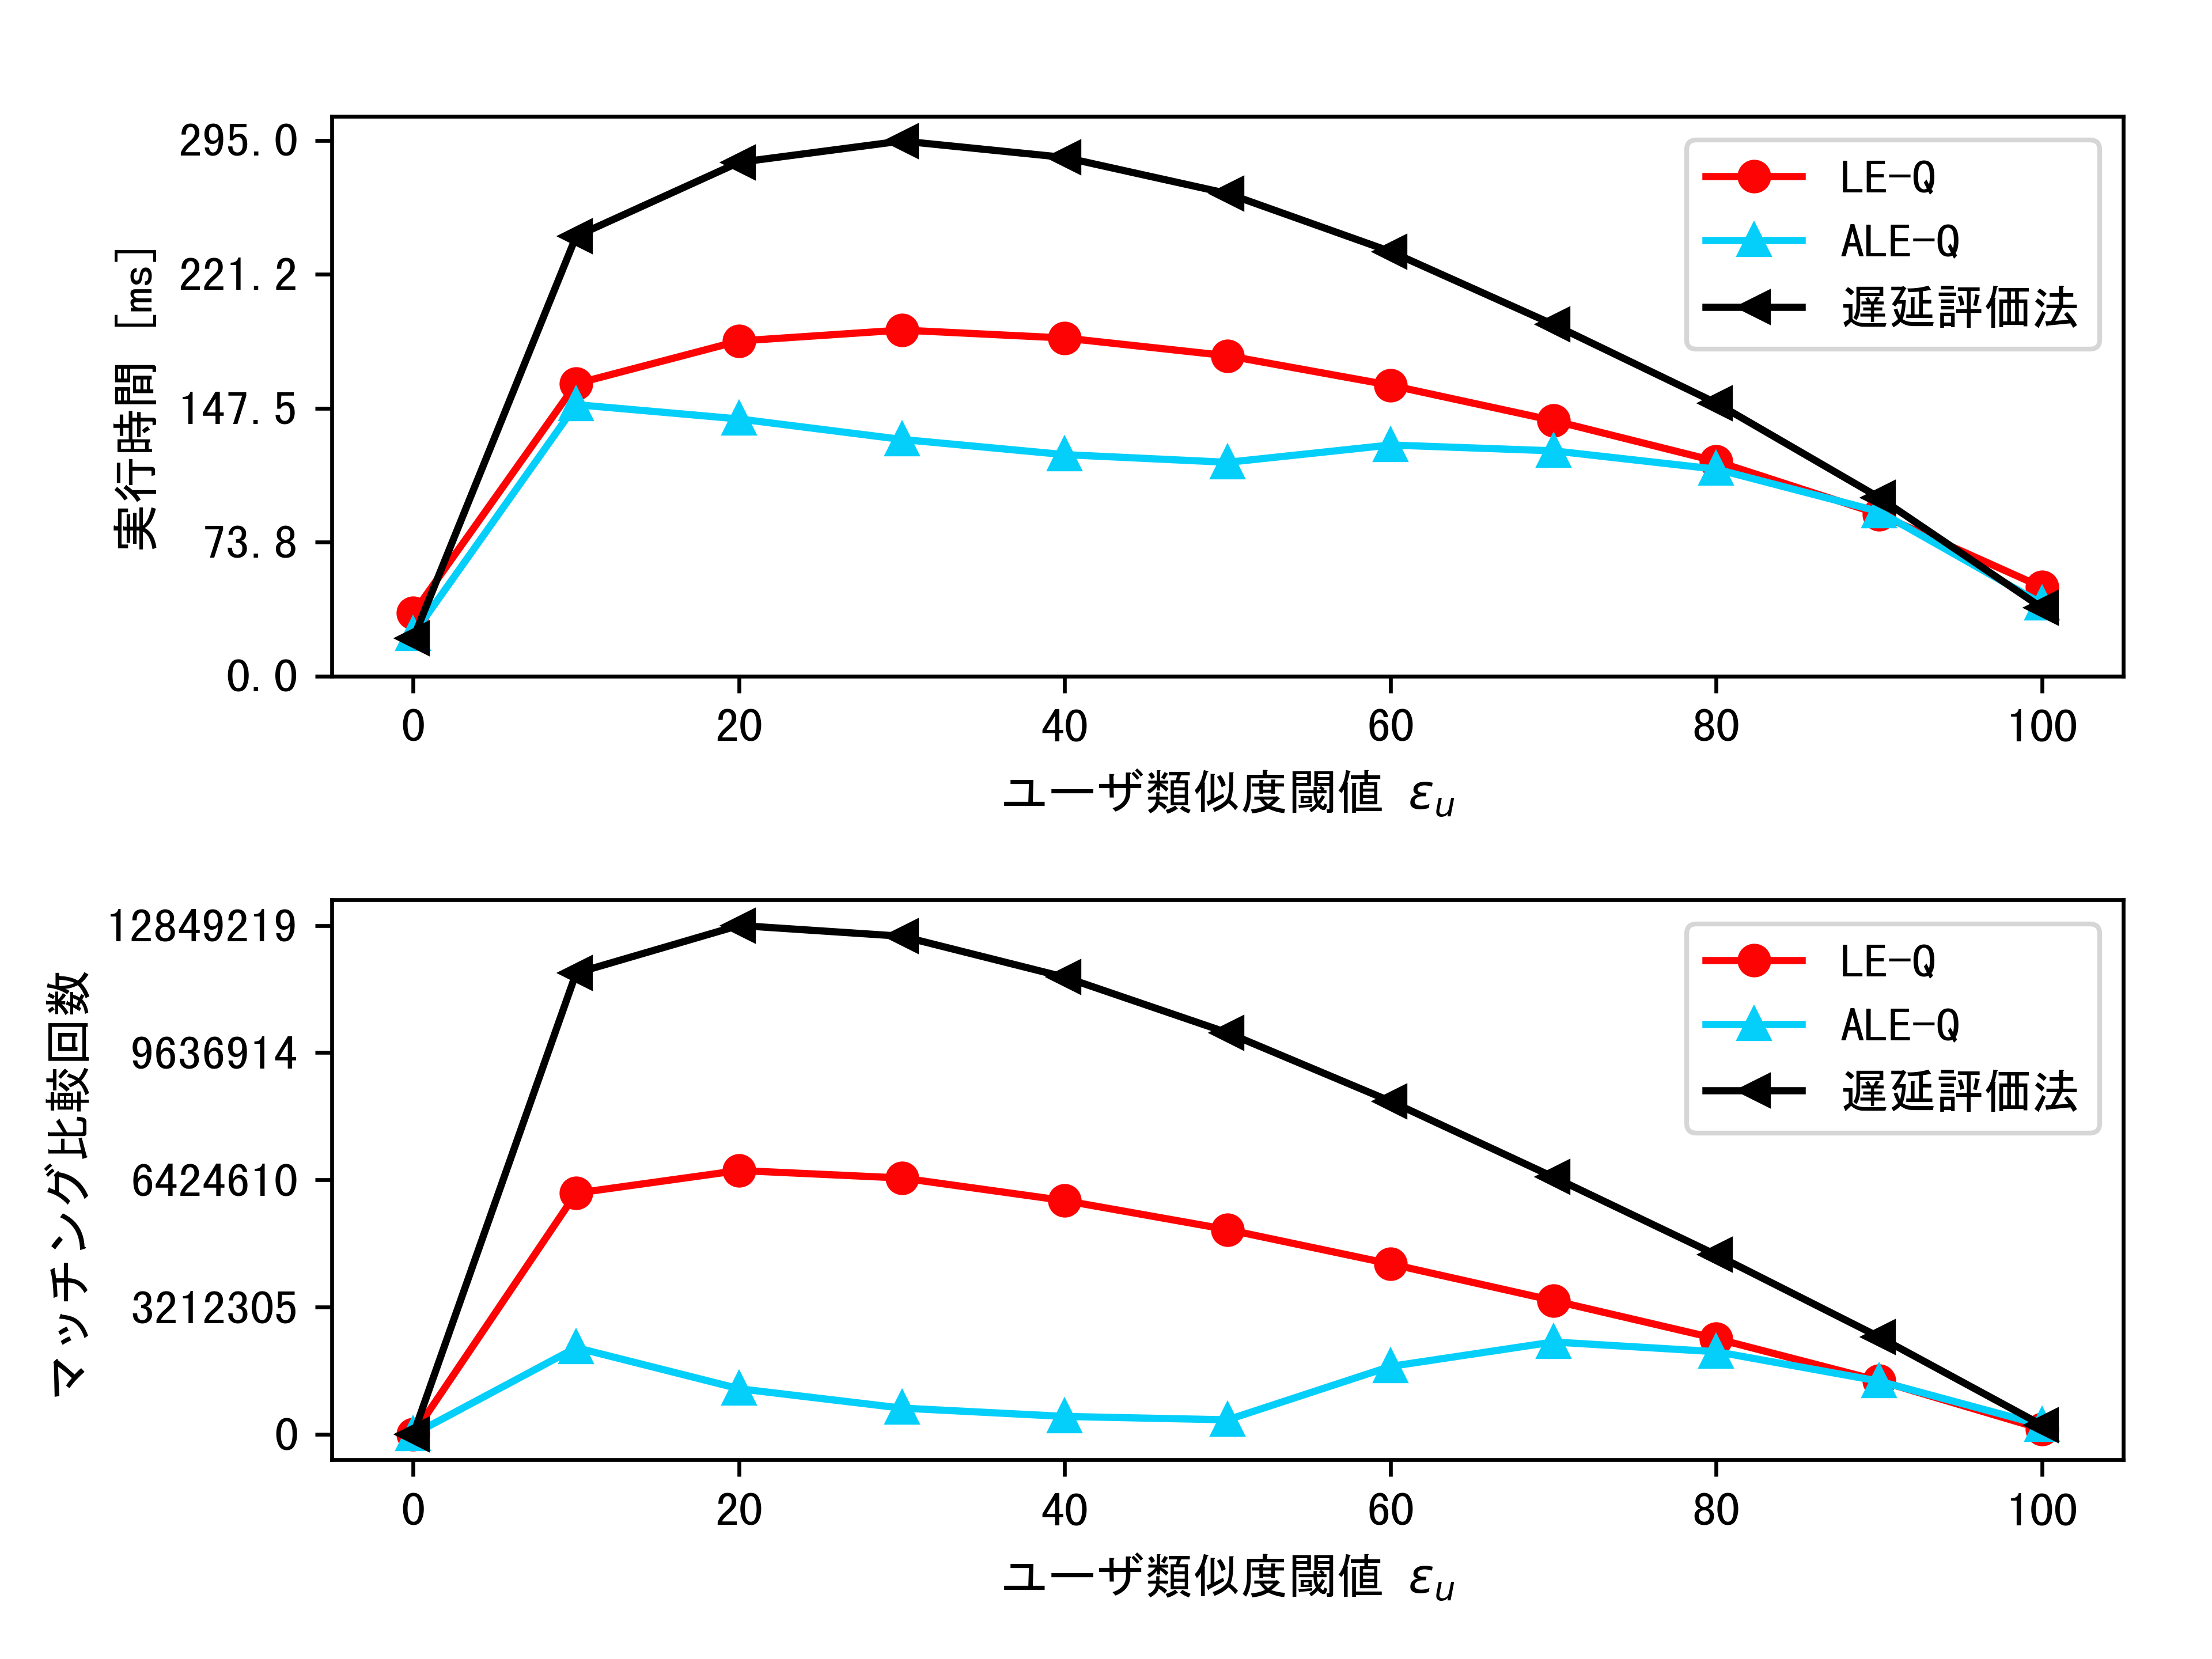
\includegraphics[width=8.3cm]{eimg/exp3.png}
    \caption{ALE-Qの性能比較(人工データセット($p=0.96^{(i-1)}$))}
    \label{fig:exp3}
\end{figure}
$\epsilon_r$を55,$\epsilon_m$を5としたCoPhIRデータセットにおける実験結果を図\ref{fig:exp3_c}に示した.人工データの実験の図\ref{fig:exp3}と同様にALE-Qの方がLE-Qより早くなっていることがわかる.
%図\ref{fig:exp3_c}は人工データによる実験と同様の結果を示し,ALE-Qは本研究で最も効率的なアルゴリズムであるといえる.
\begin{figure}[H]
    \centering
    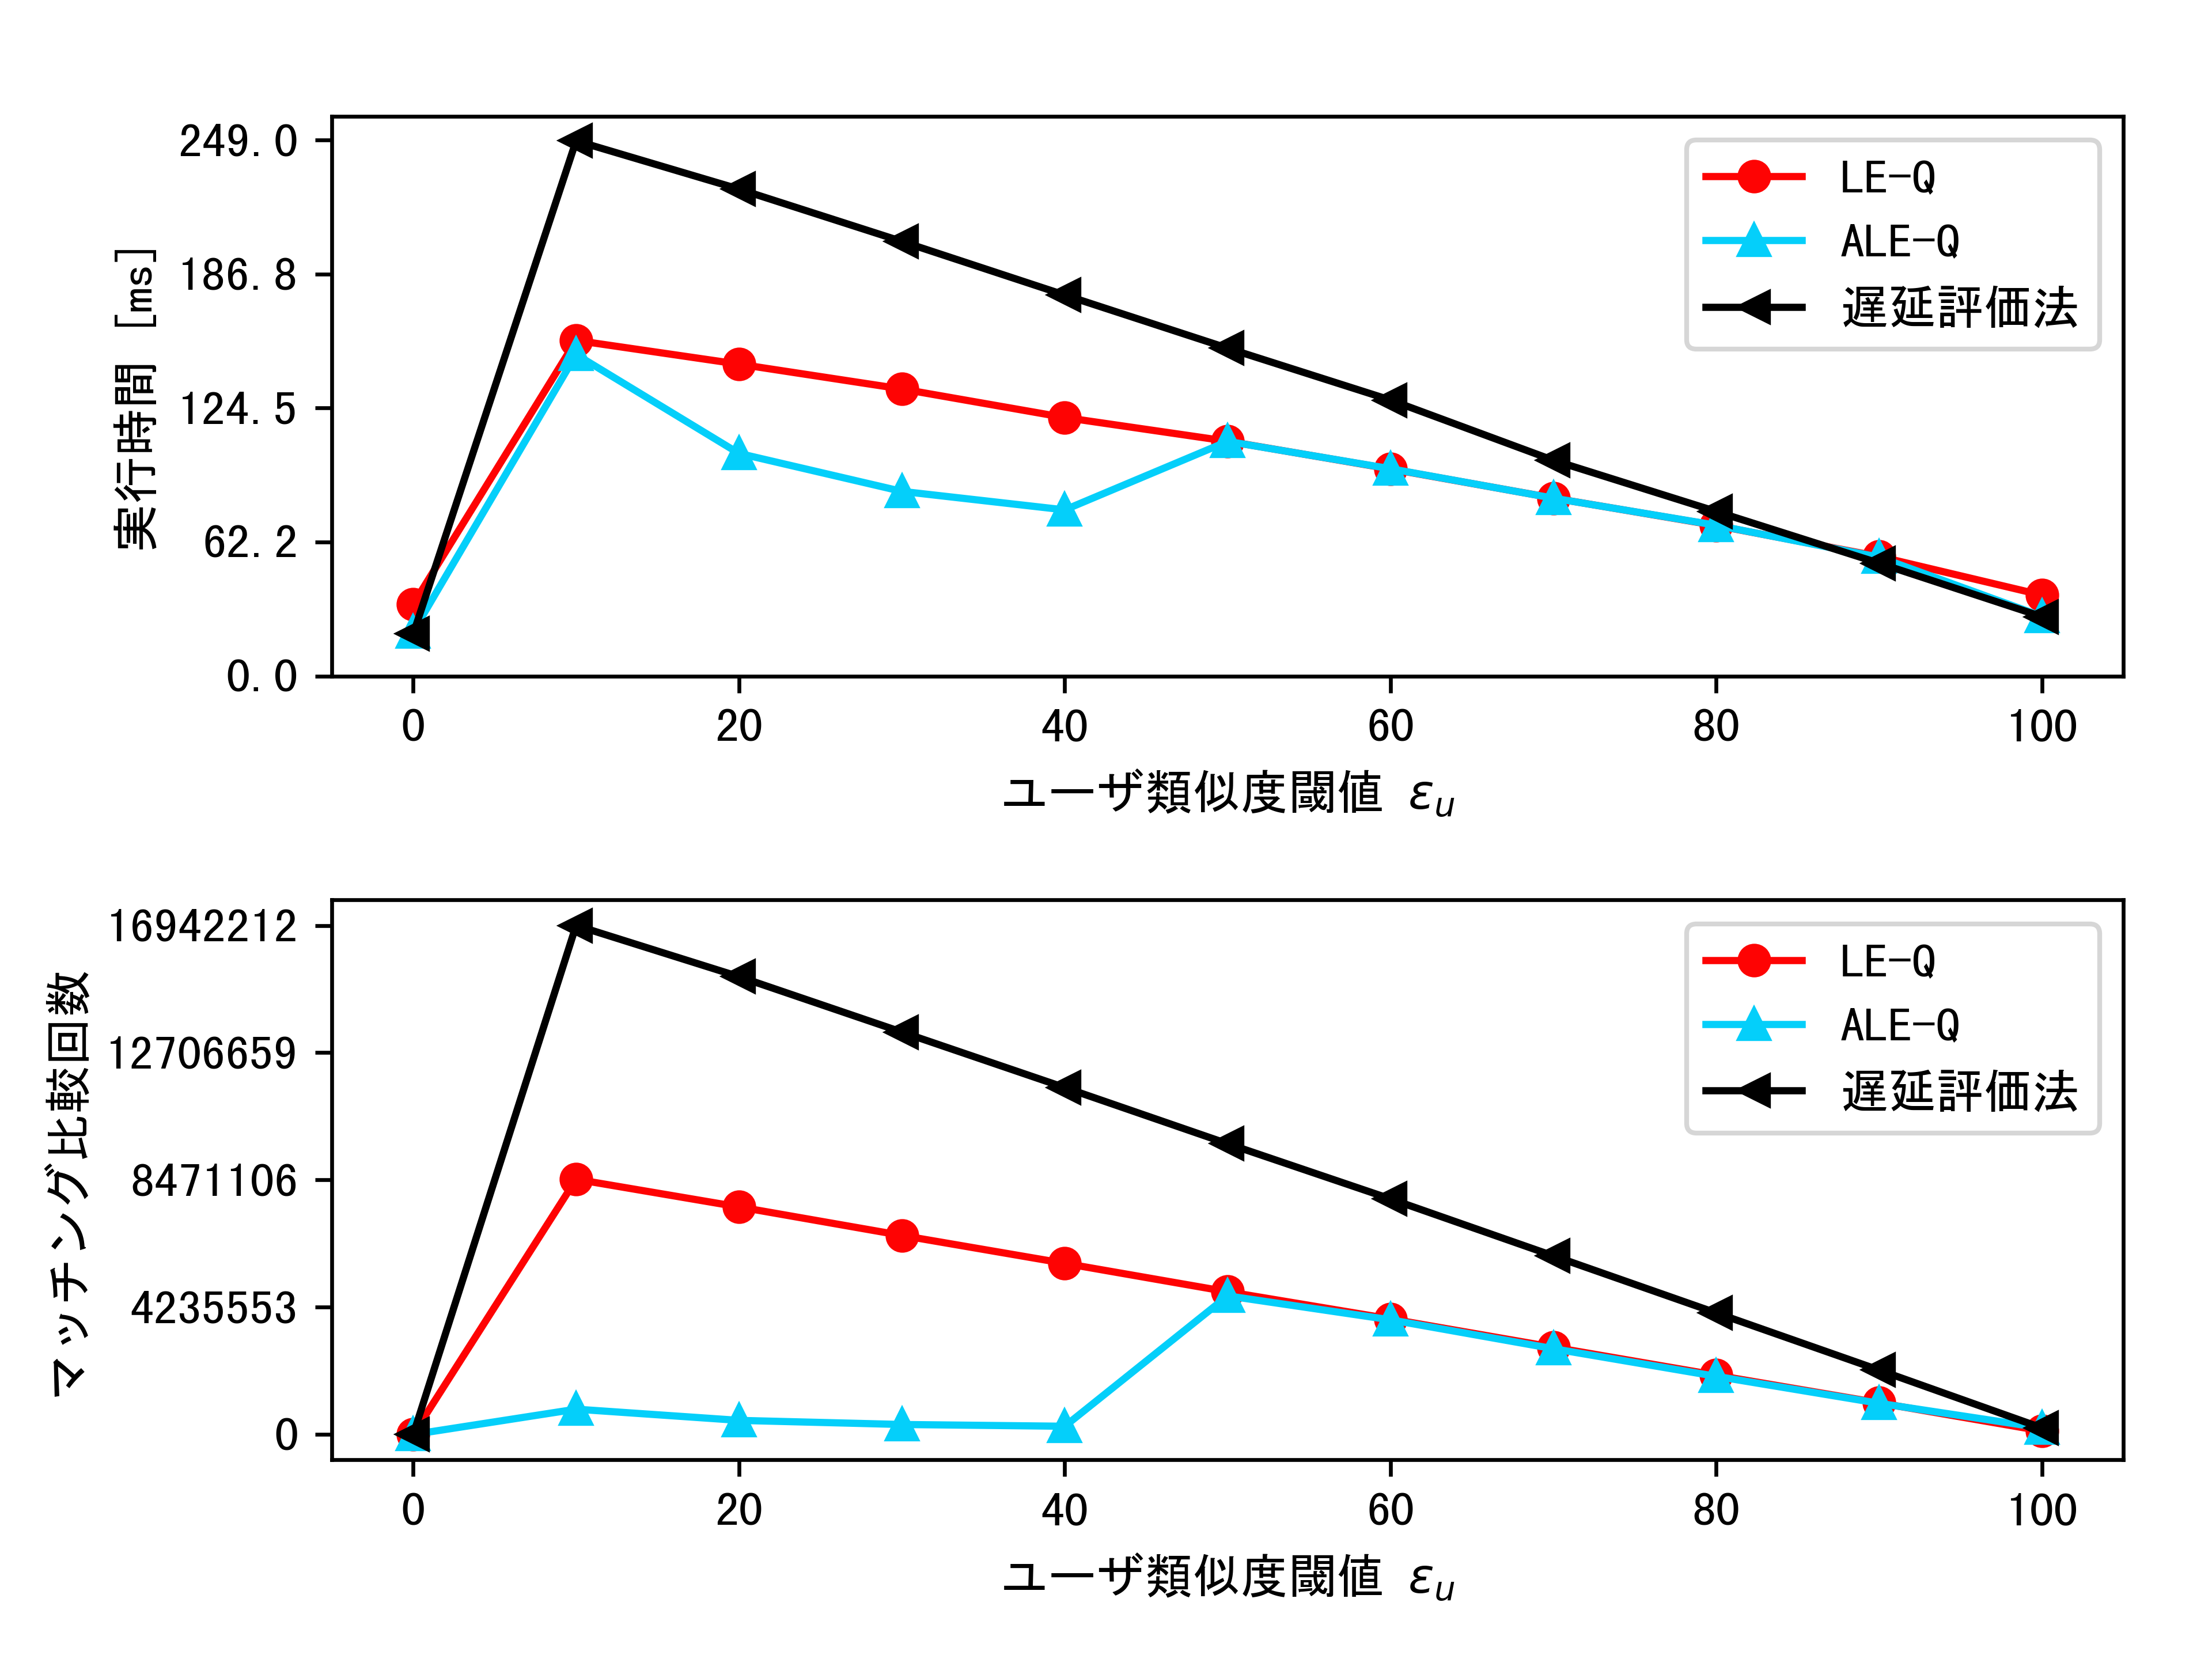
\includegraphics[width=8.3cm]{eimg/exp3_c.png}
    \caption{ALE-Qの性能比較(CoPhIRデータセット)}
    \label{fig:exp3_c}
\end{figure}

$\epsilon_r$を40,$\epsilon_m$を5としたときの人工データセットにおける$p$を固定した場合の実験結果を図\ref{fig:exp3_1},図\ref{fig:exp3_3},図\ref{fig:exp3_5},図\ref{fig:exp3_7},図\ref{fig:exp3_9}に示した.
%\ref{exp1}節ではクエリユーザに対するデータベースユーザの類似度が大きいとき遅延評価法よりLE-Qの方が実行時間が多くかかっていたが,今回の実験で改善案のALE-Qは類似度が大きい場合でも遅延評価法以下の実行時間で処理することが出来ることを示せた.
閾値$\epsilon_r$,$\epsilon_m$を用いた転置インデクス利用の切り替えを適応的に行った結果,マッチング比較回数を削減することに繋がり,$p$の値によらずLE-QよりもALE-Qの方が実行時間が短くなるという結果が示された.

\begin{figure}[H]
    \centering
    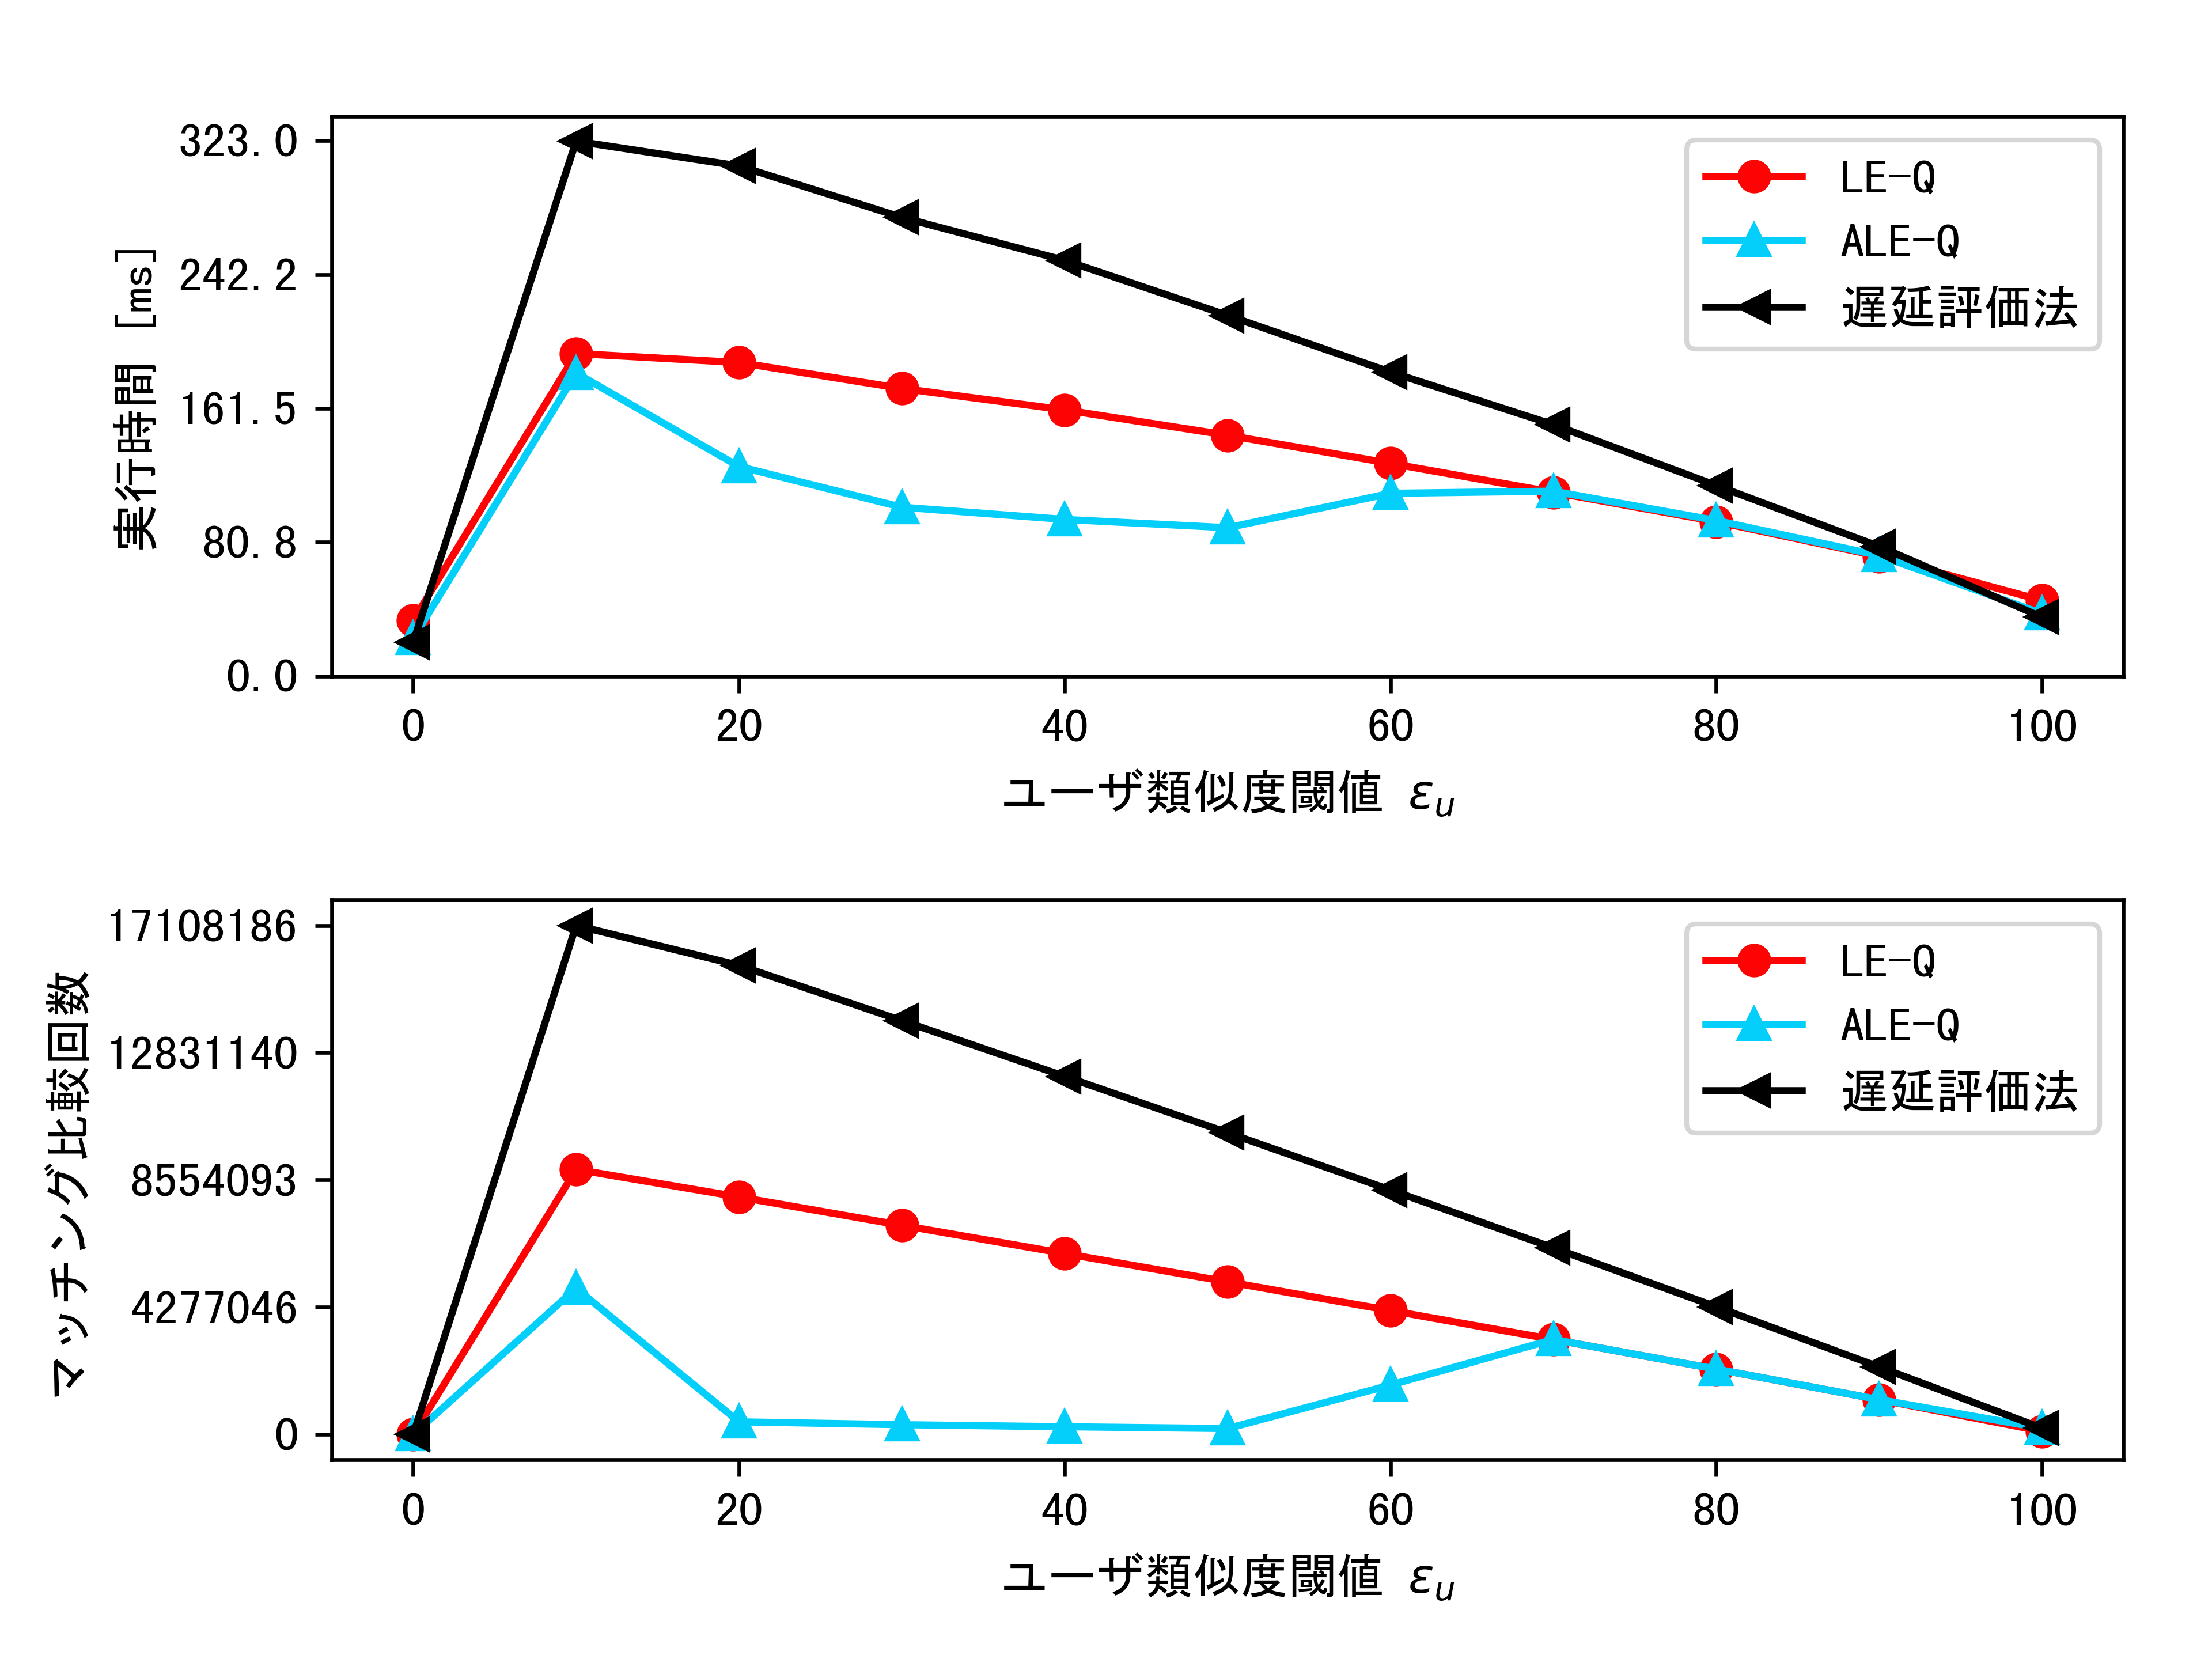
\includegraphics[width=8.3cm]{eimg/exp3_1.png}
    \caption{ALE-Qの性能比較(人工データセット($p=0.1$))}
    \label{fig:exp3_1}
\end{figure}
\begin{figure}[H]
    \centering
    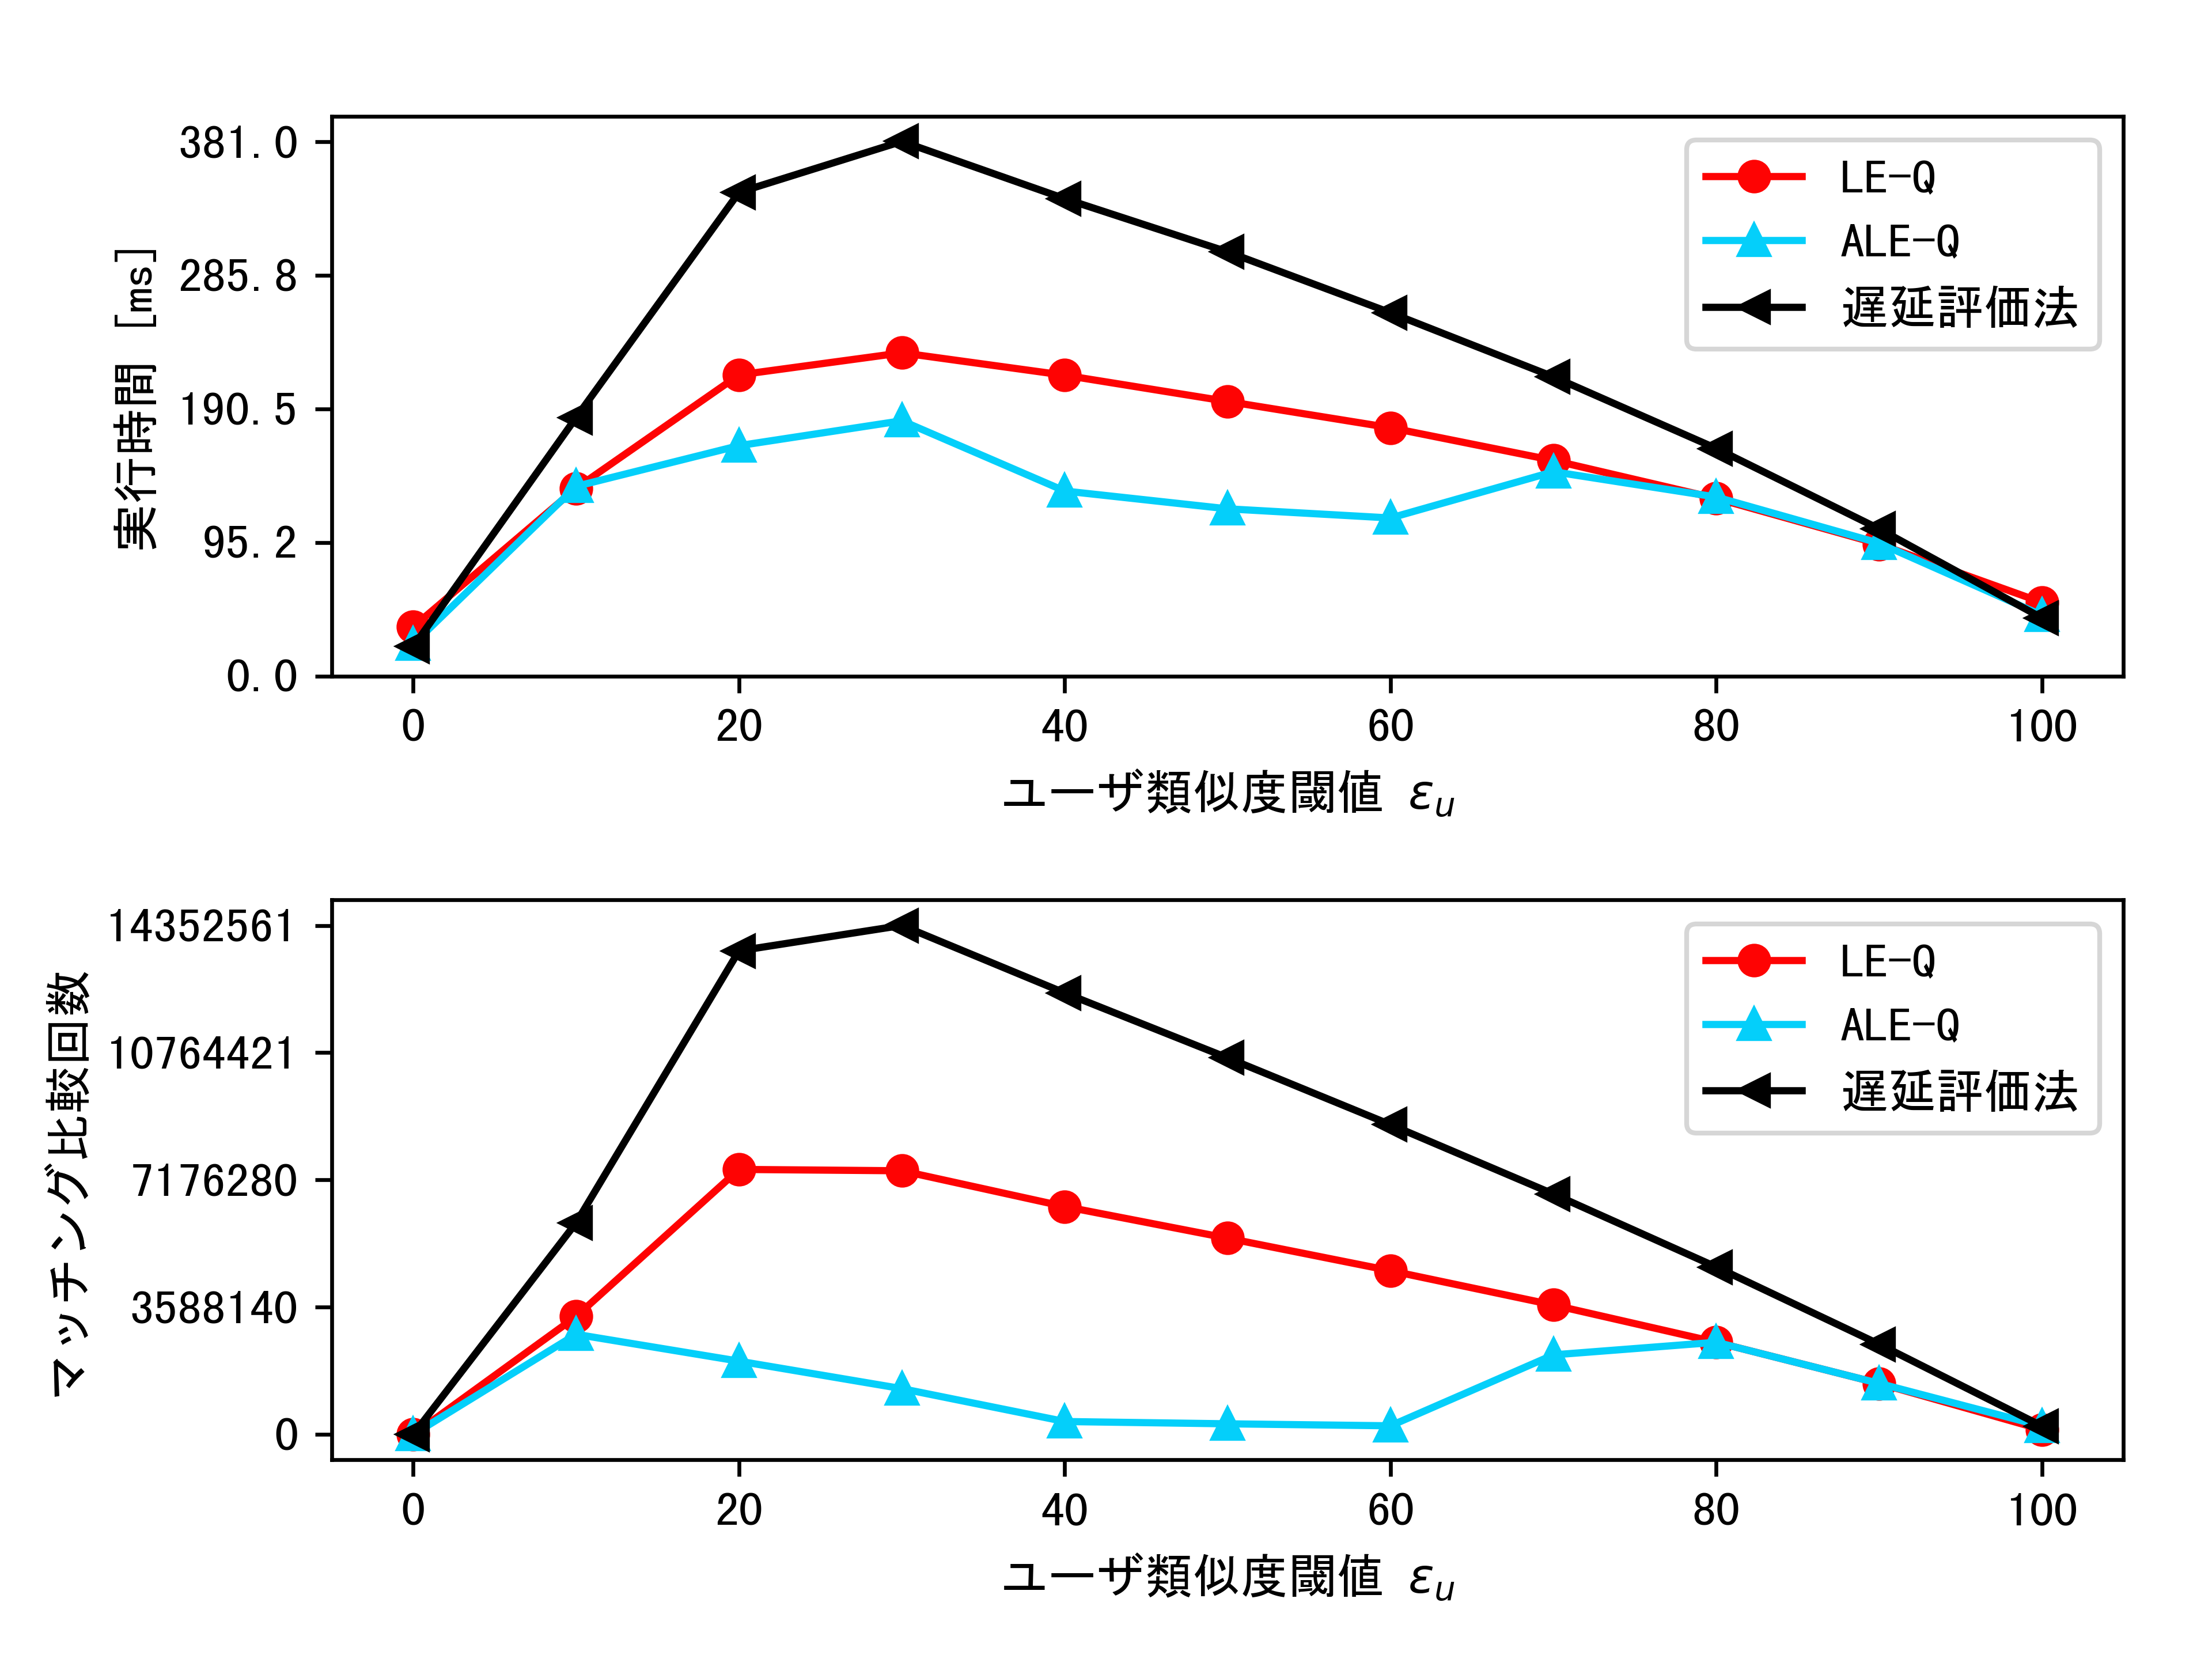
\includegraphics[width=8.3cm]{eimg/exp3_3.png}
    \caption{ALE-Qの性能比較(人工データセット($p=0.3$))}
    \label{fig:exp3_3}
\end{figure}
\begin{figure}[H]
    \centering
    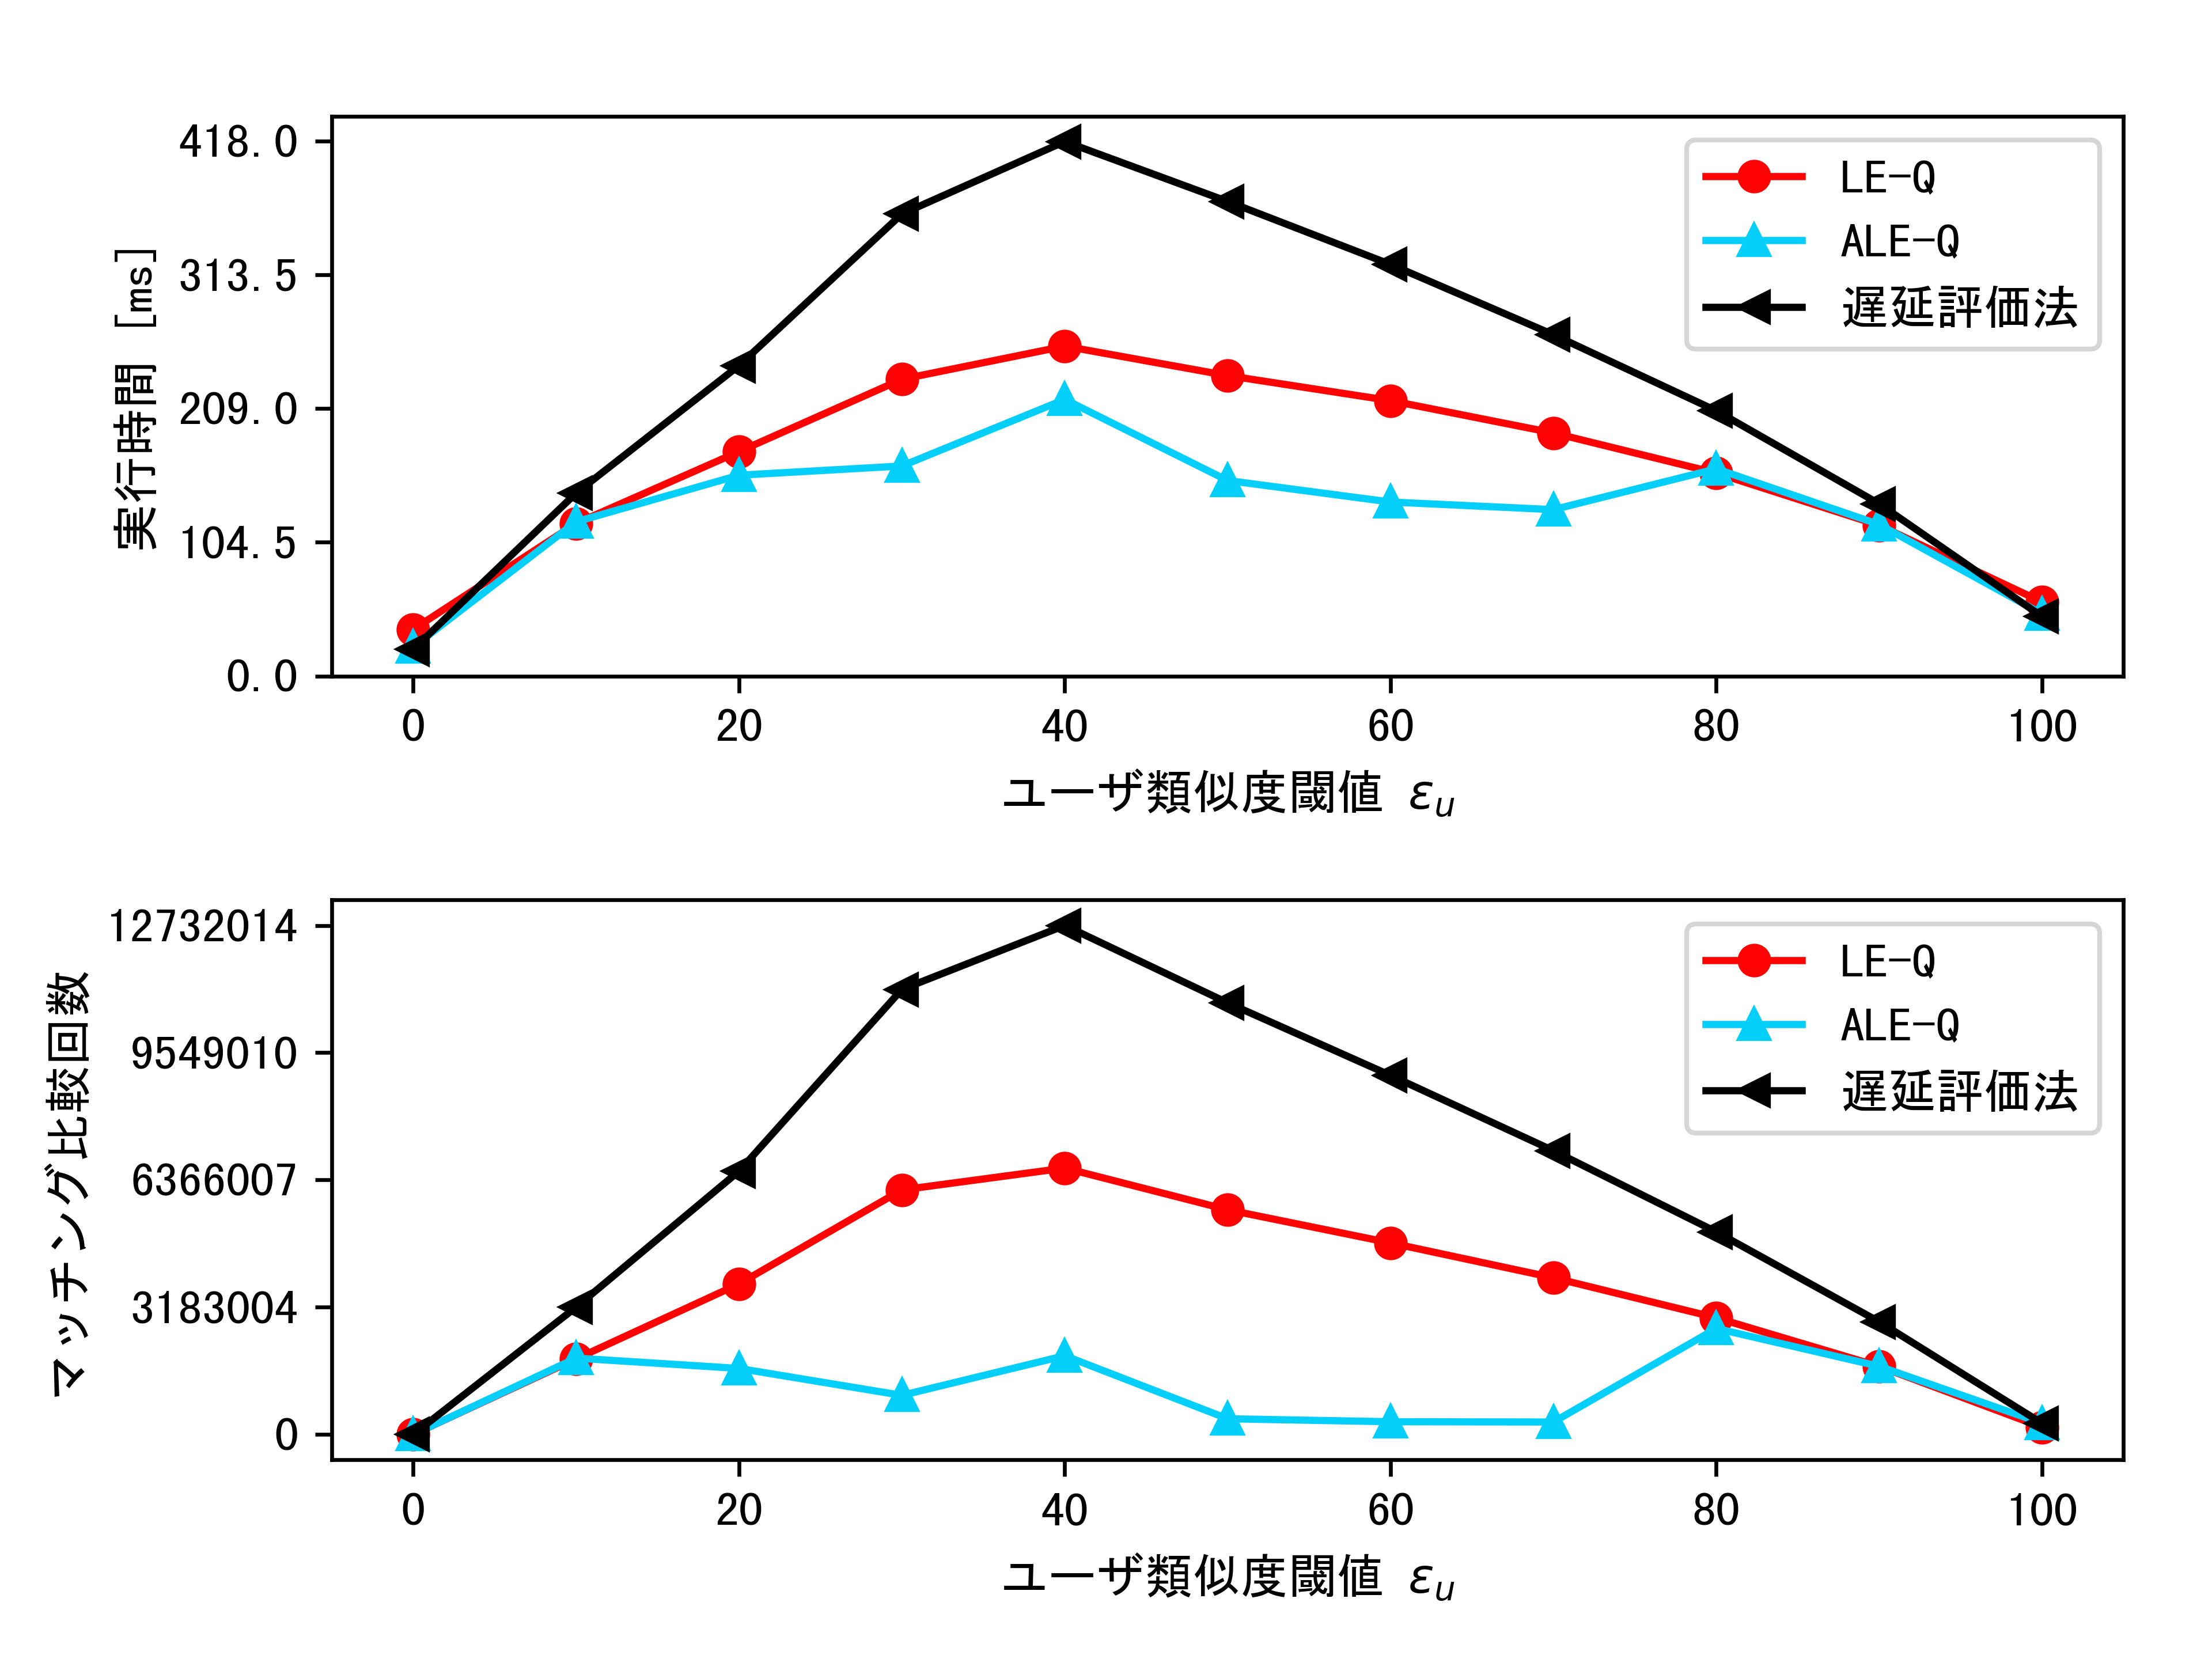
\includegraphics[width=8.3cm]{eimg/exp3_5.png}
    \caption{ALE-Qの性能比較(人工データセット($p=0.5$))}
    \label{fig:exp3_5}
\end{figure}
\begin{figure}[H]
    \centering
    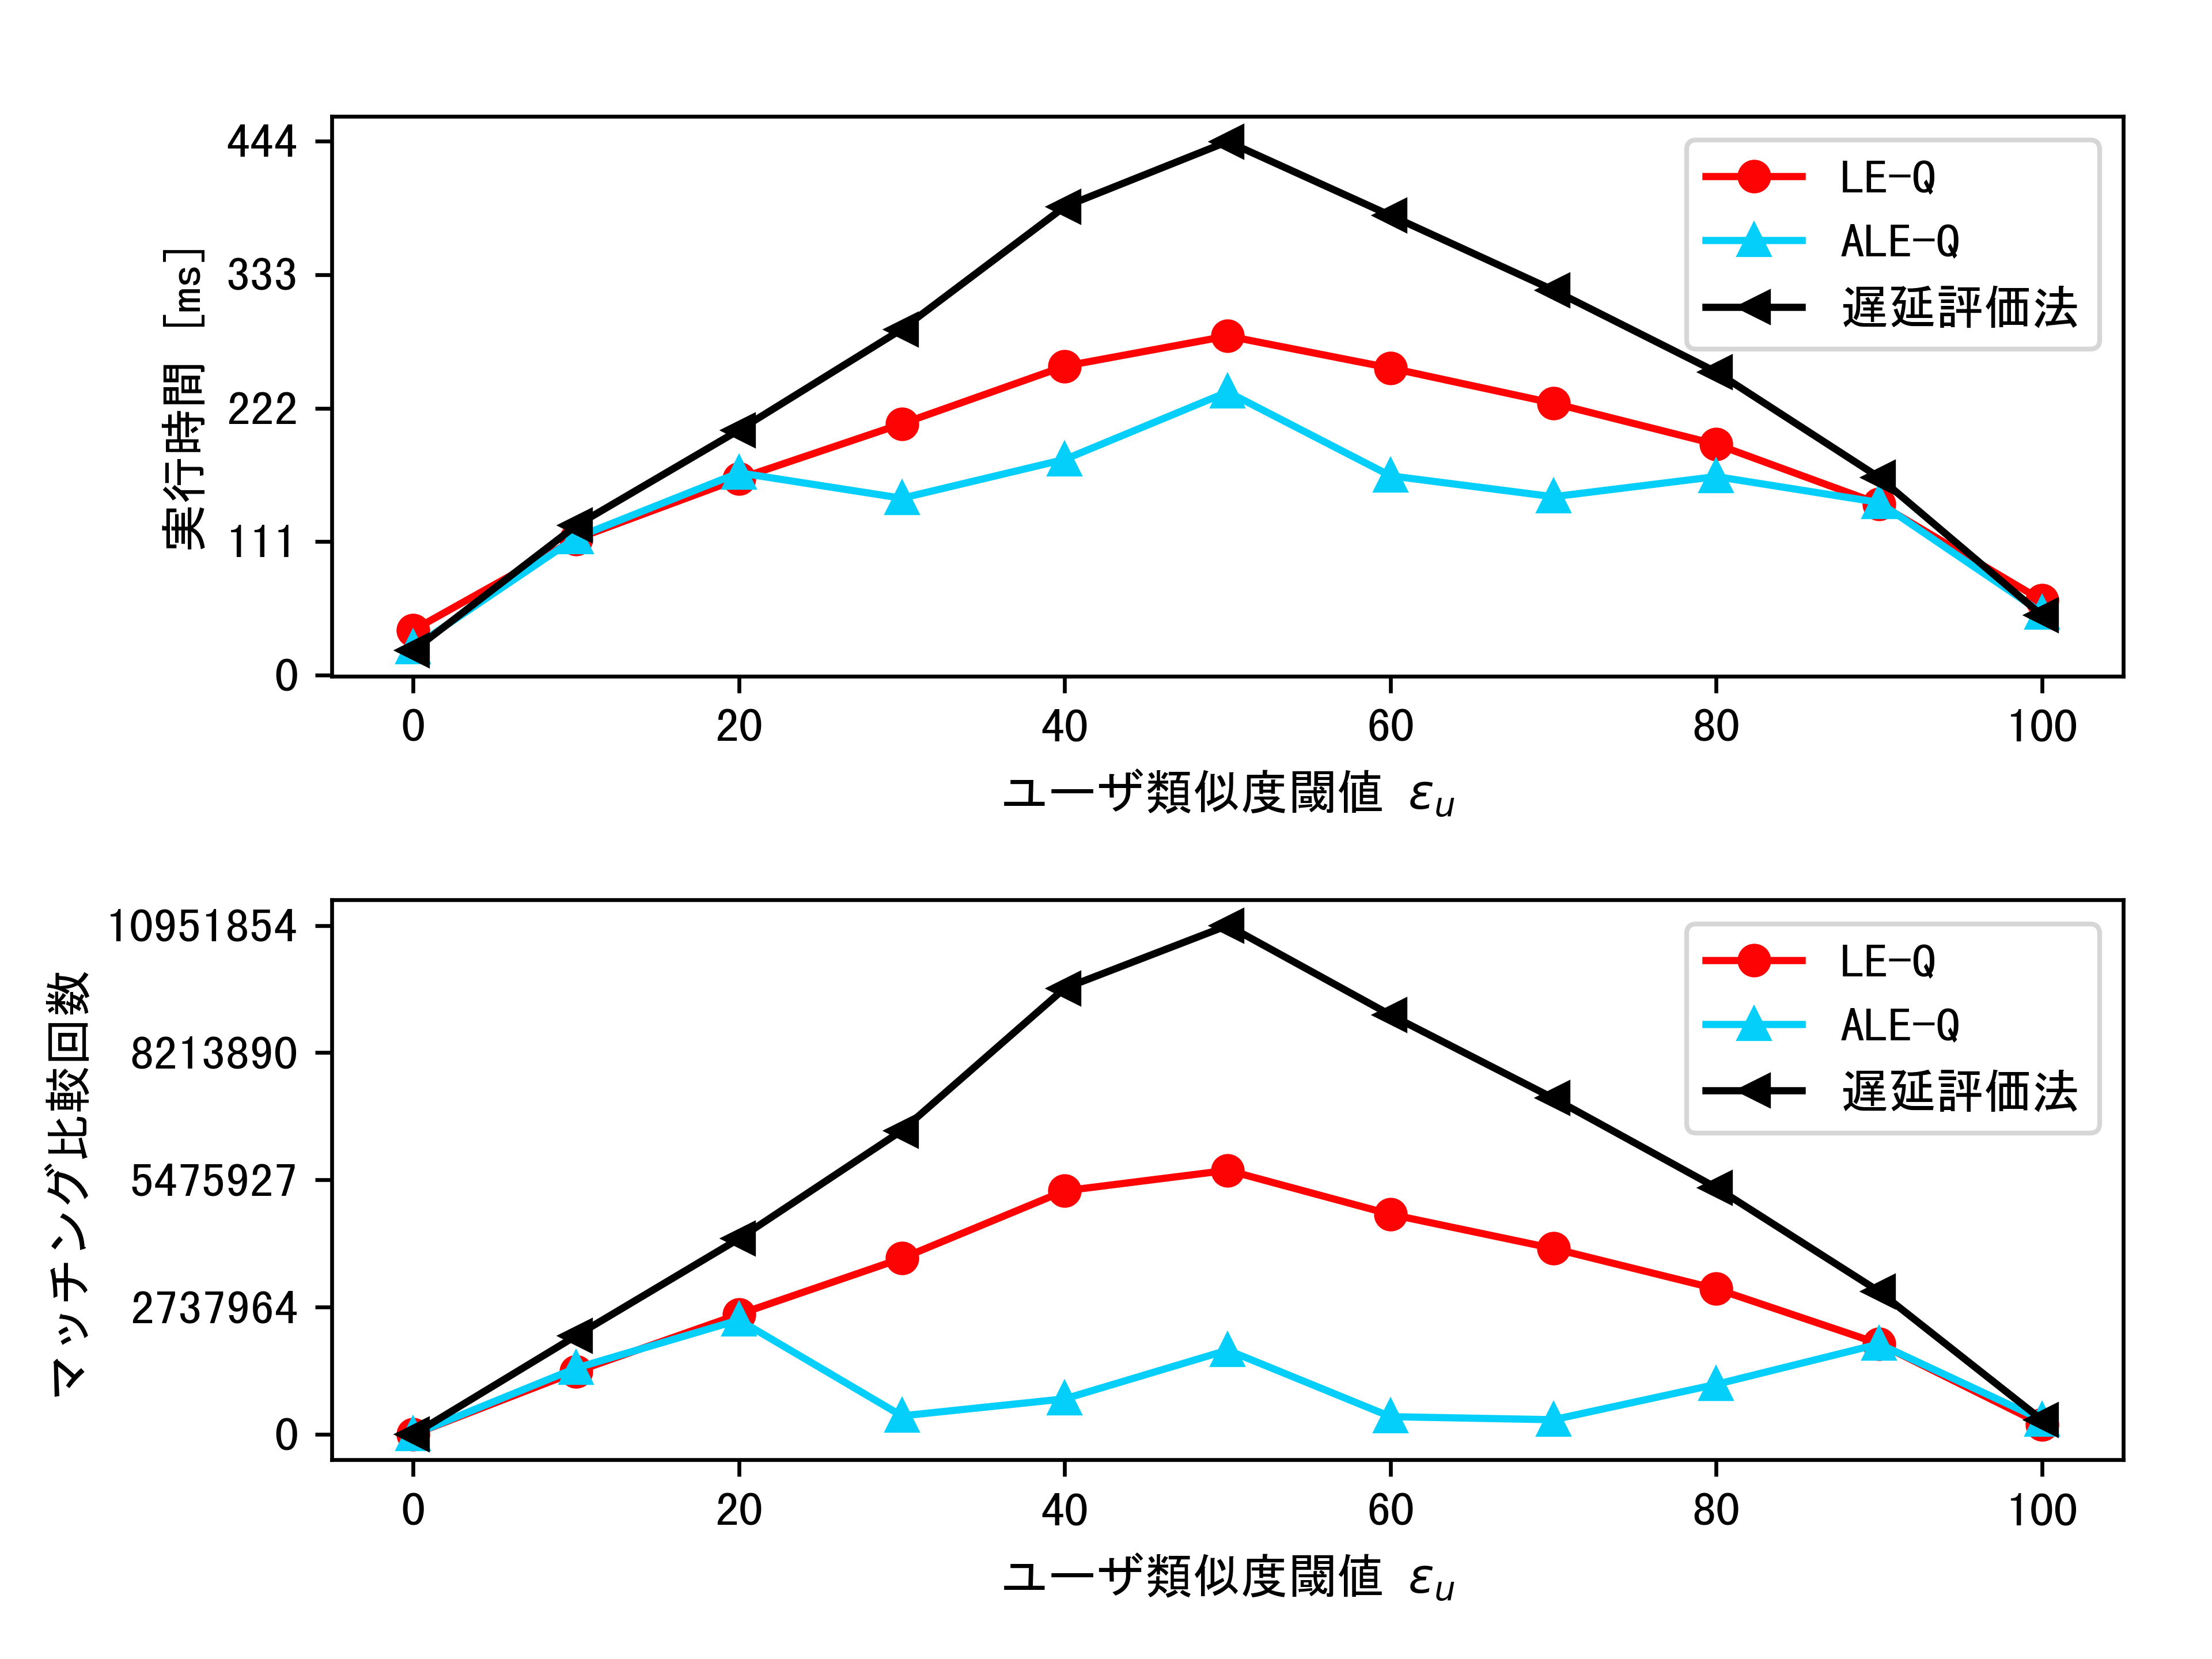
\includegraphics[width=8.3cm]{eimg/exp3_7.png}
    \caption{ALE-Qの性能比較(人工データセット($p=0.7$))}
    \label{fig:exp3_7}
\end{figure}
\begin{figure}[H]
    \centering
    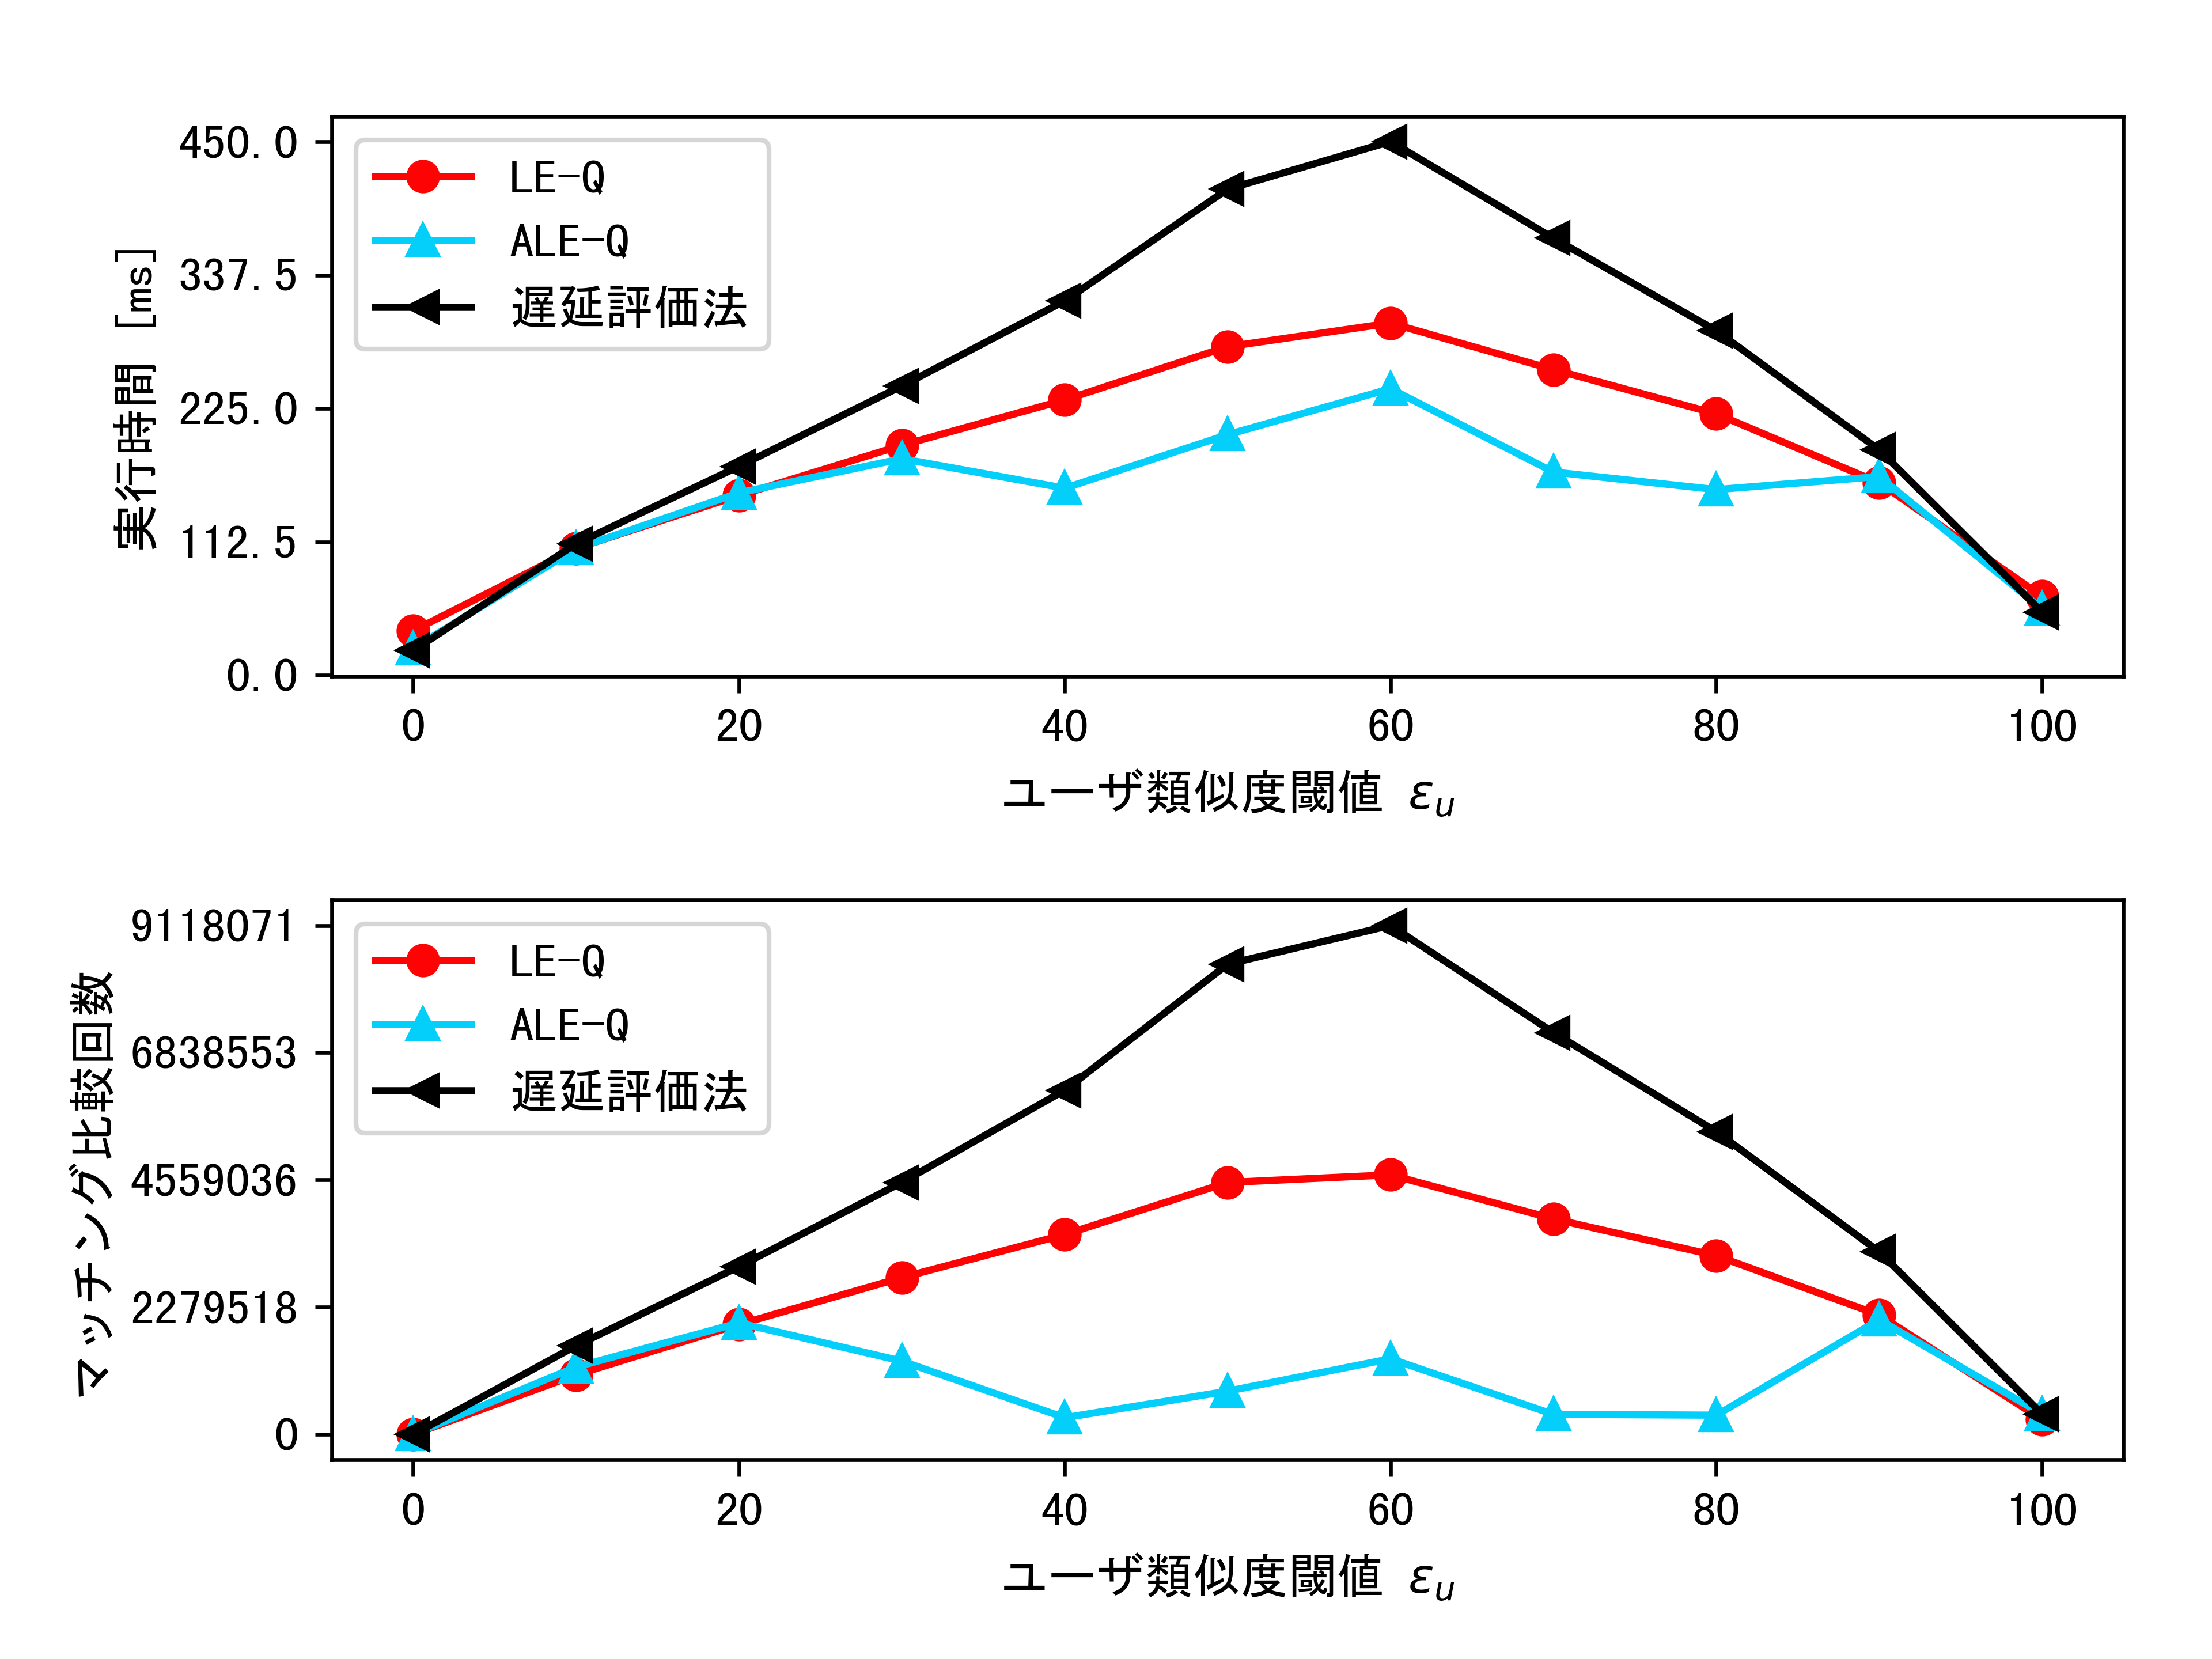
\includegraphics[width=8.3cm]{eimg/exp3_9.png}
    \caption{ALE-Qの性能比較(人工データセット($p=0.9$))}
    \label{fig:exp3_9}
\end{figure}

%よって,ALE-QをCTS問題の最も効率的なアルゴリズムであると結論付ける.

\chapter{結論}
\input{Chap9.tex}

%%ChapAcknow

\begin{acknowledgements}
    \vspace{1.0cm}
    本研究を行うにあたり,研究の場と適切なご指導,ご助言を頂いた古賀久志准教授に深く感謝いたします.また,研究室での生活や研究の様々な場面でご助言を頂きました古賀研究室の学生の皆さま,すでにご卒業された先輩方に感謝いたします.
    
    \vspace{2.0cm}
    \begin{flushright}
      令和4年1月31日
    \end{flushright}
    
\end{acknowledgements}
 %acknowledgements


%======参考文献======
 %\nocite{*} % 文献ぜんぶ載せるやつ
\bibliography{ref}
%\bibliographystyle{junsrt}

%\input{thebibliography_template.tex}%参考文献
%======付録=========
%\input{ChapAppendix.tex}
\end{document}
